\documentclass[11pt,oneside]{book}
% ==========================================================================
% preamble.tex -- shared packages, macros, and styling for the whole book
% ==========================================================================

% ---- Page geometry -------------------------------------------------------
\usepackage[paperwidth=7in,paperheight=9.25in,
            top=0.85in,bottom=0.85in,inner=0.9in,outer=0.7in]{geometry}

% ---- Fonts / encoding ------------------------------------------------------
\usepackage[utf8]{inputenc}
\usepackage[T1]{fontenc}
\usepackage{lmodern}
\usepackage{textcomp}
\usepackage{microtype}

% ---- Math ------------------------------------------------------------------
\usepackage{amsmath,amssymb,amsfonts}
\usepackage{mathtools}
\usepackage{gensymb}     % \degree, \ohm

% ---- Units (siunitx is not available in this TeX install; lightweight
%      substitute macros are defined below in "Custom macros") ------------

% ---- Graphics / color -------------------------------------------------------
\usepackage{graphicx}
\usepackage{xcolor}
\graphicspath{{img/}{../img/}}

% ---- Circuits & plots --------------------------------------------------
\usepackage{circuitikz}
\usepackage{tikz}
\usetikzlibrary{arrows.meta,positioning,calc,decorations.pathmorphing,decorations.markings,shapes.geometric,patterns}
\usepackage{pgfplots}
\pgfplotsset{compat=1.17}
\usepgfplotslibrary{groupplots}

% ---- Tables --------------------------------------------------------------
\usepackage{booktabs}
\usepackage{longtable}
\usepackage{array}
\usepackage{multirow}
\usepackage{colortbl}
\usepackage{tabularx}
\newcolumntype{Y}{>{\raggedright\arraybackslash}X}

% ---- Lists, boxes, layout -------------------------------------------------
\usepackage{enumitem}
\setlist{itemsep=2pt,topsep=4pt}
\usepackage[most]{tcolorbox}
\usepackage{titlesec}
\usepackage{fancyhdr}
\usepackage{needspace}
\usepackage{float}

% ---- References / links ---------------------------------------------------
\usepackage[colorlinks=true,linkcolor=rlinkcolor,citecolor=rlinkcolor,
            urlcolor=rurlcolor,bookmarksdepth=3,bookmarksopen=true]{hyperref}
\usepackage{cleveref}

% ==========================================================================
% Palette
% ==========================================================================
\definecolor{rblue}{HTML}{1B3A6B}
\definecolor{rorange}{HTML}{D9731E}
\definecolor{rlinkcolor}{HTML}{1B3A6B}
\definecolor{rurlcolor}{HTML}{8A4B0F}
\definecolor{rgraybg}{HTML}{F4F5F7}
\definecolor{ramber}{HTML}{FFF3D6}
\definecolor{ramberline}{HTML}{D9A320}
\definecolor{rgreenbg}{HTML}{E7F3EA}
\definecolor{rgreenline}{HTML}{2E7D46}

% ==========================================================================
% Chapter / section styling
% ==========================================================================
\titleformat{\chapter}[display]
  {\normalfont\bfseries\color{rblue}}
  {\Large\chaptertitlename~\thechapter}
  {8pt}
  {\Huge}
\titlespacing*{\chapter}{0pt}{0pt}{28pt}

\titleformat{\section}
  {\normalfont\Large\bfseries\color{rblue}}{\thesection}{8pt}{}
\titleformat{\subsection}
  {\normalfont\large\bfseries\color{rblue!80}}{\thesubsection}{8pt}{}

\pagestyle{fancy}
\fancyhf{}
\fancyhead[LE,RO]{\thepage}
\fancyhead[RE]{\nouppercase{\leftmark}}
\fancyhead[LO]{\nouppercase{\rightmark}}
\renewcommand{\headrulewidth}{0.4pt}

% ==========================================================================
% Custom macros
% ==========================================================================

% -- simple unit macro (siunitx substitute) --------------------------------
\newcommand{\unit}[1]{\,\mathrm{#1}}
\newcommand{\ohmsym}{\ensuremath{\Omega}}
\newcommand{\Wb}{\ensuremath{\mathrm{Wb}}}

% -- boxed callouts ----------------------------------------------------------
\newtcolorbox{keyidea}[1][]{
  colback=rgraybg, colframe=rblue, boxrule=0.6pt, arc=2pt,
  left=8pt, right=8pt, top=6pt, bottom=6pt,
  title={\textbf{Key Idea}\ifx&#1&\else: #1\fi}, fonttitle=\bfseries\color{white},
  colbacktitle=rblue, coltitle=white
}

\newtcolorbox{examplebox}[1][]{
  colback=rgreenbg, colframe=rgreenline, boxrule=0.6pt, arc=2pt,
  left=8pt, right=8pt, top=6pt, bottom=6pt,
  title={\textbf{Worked Example}\ifx&#1&\else: #1\fi}, fonttitle=\bfseries\color{white},
  colbacktitle=rgreenline, coltitle=white
}

\newtcolorbox{examtip}[1][]{
  colback=ramber, colframe=ramberline, boxrule=0.6pt, arc=2pt,
  left=8pt, right=8pt, top=6pt, bottom=6pt,
  title={\textbf{Exam Tip}\ifx&#1&\else: #1\fi}, fonttitle=\bfseries\color{black},
  colbacktitle=ramberline, coltitle=black
}

\newtcolorbox{safetynote}[1][]{
  colback=red!5, colframe=red!55!black, boxrule=0.6pt, arc=2pt,
  left=8pt, right=8pt, top=6pt, bottom=6pt,
  title={\textbf{Safety}\ifx&#1&\else: #1\fi}, fonttitle=\bfseries\color{white},
  colbacktitle=red!55!black, coltitle=white
}

% -- chapter-end quick review list ------------------------------------------
\newenvironment{quickreview}
  {\bigskip\noindent\textbf{\large\color{rblue}Chapter Review}\par\smallskip
   \begin{itemize}[leftmargin=*]}
  {\end{itemize}}

\newenvironment{practiceproblems}
  {\bigskip\noindent\textbf{\large\color{rblue}Practice Problems}\par\smallskip
   \begin{enumerate}[leftmargin=*]}
  {\end{enumerate}}

% figure helper
\newcommand{\bookfig}[3][0.62]{%
  \begin{figure}[H]
    \centering
    \includegraphics[width=#1\linewidth]{#2}
    \caption{#3}
  \end{figure}
}


\title{The Complete Amateur Radio Operator}
\author{Radio School Press}
\date{2026 Edition}

\begin{document}

\begin{titlepage}
\centering
\vspace*{1.2in}
{\Huge\bfseries\color{rblue} The Complete\\[4pt] Amateur Radio Operator\par}
\vspace{0.4in}
{\Large\color{rorange} Theory, Technology, and Practice for the Modern Ham\par}
\vspace{1in}
{\large A self-contained course in the physics, electronics, and operating\\
practice of amateur (``ham'') radio --- written to prepare a motivated\\
reader for \emph{any} country's licensing examinations, from first\\
principles to advanced RF engineering.\par}
\vfill
{\large 2026 Edition\par}
\vspace{0.2in}
{\normalsize Radio School Press\par}
\end{titlepage}


\frontmatter
\chapter*{Preface}
\addcontentsline{toc}{chapter}{Preface}
\markboth{Preface}{Preface}

Amateur (``ham'') radio sits at a rare intersection: it is simultaneously a
hands-on engineering discipline, an experimental science, a public-service
tradition, and a global community held together by little more than
electromagnetic waves and a shared curiosity about how things work. Every
licensed amateur, anywhere in the world, has had to learn the same
underlying physics --- Ohm's law does not change at a border, and a
half-wave dipole behaves identically whether it is strung between two trees
in Lisbon, Nairobi, or Auckland.

This book was written to teach that underlying physics and engineering as
completely and rigorously as a motivated newcomer needs, independent of
where they happen to live. National licensing authorities differ enormously
in their exam formats, their band allocations, their power limits, and the
paperwork required to get on the air --- and this book intentionally does
\emph{not} try to teach any single country's regulations. Instead, it
teaches the physics, mathematics, electronics, antenna theory, propagation,
and operating practice that sit underneath \emph{every} national exam
syllabus, so that the material remains useful and accurate regardless of
which administration issues your callsign. Where a topic is genuinely
international --- the ITU Region system, the Q-code, the NATO phonetic
alphabet, Morse operating abbreviations --- it is covered in full, because
these are shared worldwide conventions rather than local law.

The book is organized in five parts of increasing sophistication, loosely
mirroring the tiered structure used by most national licensing systems
(an entry-level tier, an intermediate tier, and a full-privileges tier),
so that a reader preparing for a foundation-level exam can stop after
Part~II with a solid, self-sufficient understanding, while a reader aiming
for the highest available privileges can continue through the treatment of
active devices, transmission line theory, antenna engineering, and
propagation in Parts~III and~IV. Part~V turns from theory to practice:
operating procedure, radio etiquette, digital modes, and emergency
communications, all described in terms general enough to apply to any
amateur service worldwide.

Because exam questions ultimately test whether you can \emph{use} a
formula, not just recite it, every chapter includes worked examples,
exam-style tips, and end-of-chapter review questions. A comprehensive
formula appendix (Appendix~A) collects every equation in the book in one
place for quick reference and last-minute revision, alongside a table of
physical constants, SI prefixes, and unit conversions (Appendix~B) and a
glossary of terms (Appendix~C).

Before you use this book to sit a real examination, confirm the specific
band plan, power limits, callsign format, and administrative procedure
that apply in your own country with your national telecommunications
regulator or IARU member society --- those details are the one part of
becoming a radio amateur that genuinely does depend on where you live.

Good luck, and 73.

\chapter*{How to Use This Book}
\addcontentsline{toc}{chapter}{How to Use This Book}
\markboth{How to Use This Book}{How to Use This Book}

\textbf{Reading tiers.} Chapters are grouped into five parts. Parts~I and~II
correspond roughly to the depth expected of an entry-level (``foundation''
or ``novice''-class) license worldwide. Parts~III and part of~IV add the
depth typically expected of an intermediate (``technician'' or
``general''-class) license. The remainder of Part~IV and all of Part~V,
together with the full formula appendix, correspond to the depth expected
of the highest license class most administrations offer (often called
``advanced,'' ``extra,'' or ``full''). You do not need to read the parts
in lockstep with a specific national syllabus --- read as far as your
target license requires, then treat the rest as a reference to return to.
Part~VI is different in kind from the rest of the book: it is not exam
material at all, but an enrichment chapter applying the same radio
science to aviation, maritime, and military signals now commonly
explored with inexpensive SDR receivers.

\medskip
\noindent Throughout the book you will find four recurring boxes:

\begin{keyidea}
A concept worth memorizing verbatim, because it recurs across many later
chapters or is a favorite target of exam questions.
\end{keyidea}

\begin{examplebox}
A fully worked numerical problem, solved step by step, in the style of a
typical exam question.
\end{examplebox}

\begin{examtip}
A practical hint about how a topic tends to be tested, or a common mistake
to avoid.
\end{examtip}

\begin{safetynote}
A warning about a genuine electrical, RF-exposure, or mechanical hazard.
Safety notes are not exam trivia --- treat them as seriously as you would
a warning label on a piece of test equipment.
\end{safetynote}

\medskip
\noindent Each chapter closes with a \textbf{Chapter Review} (a condensed
list of the ideas you should be able to restate from memory) and a set of
\textbf{Practice Problems} with the reasoning needed to solve them found in
the chapter body. Appendix~A gathers every formula in the book by topic;
Appendix~B gathers SI prefixes, unit conversions, and physical constants;
Appendix~C is a glossary. Bookmark all three --- you will use them long
after you pass an exam.

\tableofcontents

\mainmatter

\part{Mathematical and Physical Foundations}
\chapter{Units and Measurement}
\label{ch:units}

Radio engineering spans an enormous numerical range: a weak-signal
moonbounce contact may involve powers of $10^{-21}\,\text{W}$ at the
receiver input, while a broadcast transmitter may radiate $10^{6}\,\text{W}$.
Working comfortably across eighteen or more orders of magnitude requires a
disciplined system of units and prefixes. This chapter establishes that
system before any circuit theory is introduced.

\section{The International System of Units (SI)}

Nearly all quantities used in electronics and radio are expressed in the
\textbf{International System of Units (SI)}. SI defines seven base units,
of which four are used constantly in this book:

\begin{center}
\begin{tabular}{@{}lll@{}}
\toprule
Quantity & Unit & Symbol \\
\midrule
Length & metre & m \\
Mass & kilogram & kg \\
Time & second & s \\
Electric current & ampere & A \\
\bottomrule
\end{tabular}
\end{center}

Every other electrical quantity used in this book --- voltage, resistance,
capacitance, inductance, power, frequency --- is a \emph{derived} unit,
built from these base units. For example, the volt is defined so that one
ampere flowing through one ohm of resistance produces a potential
difference of one volt; the ohm itself is defined in terms of volts and
amperes. You do not need to memorize these base-unit derivations, but
understanding that all electrical units are ultimately tied to the same
consistent system explains why formulas in this book always balance: if
you put SI units in, you get SI units out, with no hidden conversion
factors.

\begin{center}
\begin{tabular}{@{}llll@{}}
\toprule
Quantity & Unit & Symbol & In base SI units \\
\midrule
Frequency & hertz & Hz & $\text{s}^{-1}$ \\
Force & newton & N & $\text{kg}\cdot\text{m}\cdot\text{s}^{-2}$ \\
Energy & joule & J & $\text{N}\cdot\text{m}$ \\
Power & watt & W & $\text{J}/\text{s}$ \\
Charge & coulomb & C & $\text{A}\cdot\text{s}$ \\
Potential difference & volt & V & $\text{J}/\text{C}$ \\
Resistance & ohm & $\Omega$ & $\text{V}/\text{A}$ \\
Capacitance & farad & F & $\text{C}/\text{V}$ \\
Inductance & henry & H & $\text{V}\cdot\text{s}/\text{A}$ \\
Magnetic flux & weber & Wb & $\text{V}\cdot\text{s}$ \\
Magnetic flux density & tesla & T & $\text{Wb}/\text{m}^2$ \\
\bottomrule
\end{tabular}
\end{center}

\section{SI Prefixes}
\label{sec:si-prefixes}

Rather than writing very large or very small numbers with long strings of
zeros, SI defines a standard set of prefixes, each representing a power of
ten. A radio amateur must be completely fluent with the prefixes from
pico to giga; they appear on every data sheet, every dial, and in most
exam numerical questions.

\begin{center}
\begin{tabular}{@{}lllr@{}}
\toprule
Prefix & Symbol & Factor & Example \\
\midrule
tera & T & $10^{12}$ & 1\,THz (far above amateur bands) \\
giga & G & $10^{9}$ & 2.4\,GHz (Wi-Fi/amateur microwave) \\
mega & M & $10^{6}$ & 14.2\,MHz (a 20\,m band frequency) \\
kilo & k & $10^{3}$ & 3.5\,k$\Omega$ resistor \\
--- & --- & $10^{0}$ & base unit (V, A, $\Omega$, Hz, F, H, W) \\
milli & m & $10^{-3}$ & 100\,mA current \\
micro & $\mu$ & $10^{-6}$ & 100\,$\mu$F capacitor \\
nano & n & $10^{-9}$ & 10\,nH inductor \\
pico & p & $10^{-12}$ & 22\,pF trimmer capacitor \\
\bottomrule
\end{tabular}
\end{center}

\begin{keyidea}[Prefix arithmetic]
To convert between prefixes, multiply or divide by the ratio of their
powers of ten. For example, $2\,\text{mA} = 2\times10^{-3}\,\text{A} =
2000\,\mu\text{A}$. When in doubt, always convert back to the base unit
(no prefix) before doing arithmetic, then convert the answer to a
convenient prefix at the end.
\end{keyidea}

\begin{examplebox}[Converting units]
A capacitor is labeled 4700\,pF. Express this value in microfarads and in
farads.

\emph{Solution.} $1\,\text{pF} = 10^{-12}\,\text{F}$ and
$1\,\mu\text{F} = 10^{-6}\,\text{F}$, so
$1\,\text{pF} = 10^{-6}\,\mu\text{F}$. Therefore
\[
4700\,\text{pF} = 4700 \times 10^{-6}\,\mu\text{F} = 4.7\times10^{-3}\,\mu\text{F} = 0.0047\,\mu\text{F},
\]
and in base units, $4700\,\text{pF} = 4.7\times10^{-9}\,\text{F} = 4.7\,\text{nF}$.
\end{examplebox}

\section{Scientific and Engineering Notation}

\textbf{Scientific notation} writes a number as $a \times 10^{n}$ with
$1 \le a < 10$. \textbf{Engineering notation} is a variant that restricts
$n$ to multiples of 3, so the exponent always lines up with an SI prefix
--- this is the form used on virtually all electronic calculators and test
equipment. For example, $47{,}000\,\Omega$ is $4.7\times10^{4}\,\Omega$ in
scientific notation but $47\times10^{3}\,\Omega = 47\,\text{k}\Omega$ in
engineering notation. Learn to think in engineering notation; it maps
directly onto the prefix table above.

\section{Significant Figures and Measurement Uncertainty}

No physical measurement is perfectly exact. A digital multimeter reading
of ``14.235\,MHz'' implies a different precision than ``14.2\,MHz,'' even
though both could describe the same signal. The number of \textbf{significant
figures} in a stated value indicates how precisely it is known:

\begin{itemize}
\item All non-zero digits are significant.
\item Zeros between non-zero digits are significant (1002 has four).
\item Leading zeros are never significant (0.0042 has two).
\item Trailing zeros after a decimal point are significant (3.50 has three).
\end{itemize}

When multiplying or dividing measured quantities, the result should be
rounded to the same number of significant figures as the least precise
input. This matters on exams that give component values ``as measured''
rather than as nominal (ideal) values, and it matters in the workshop when
deciding how much precision a calculation actually deserves.

\section{Logarithms: The Mathematics Behind the Decibel}

Radio engineers constantly compare quantities that range over many orders
of magnitude --- transmitter power versus receiver sensitivity, for
example. The tool for compressing such ratios into manageable numbers is
the \textbf{logarithm}, formally introduced here because it underlies the
decibel system developed in Chapter~\ref{ch:decibels}.

For a base-10 logarithm,
\[
y = \log_{10}(x) \iff 10^{y} = x .
\]
Three properties make logarithms indispensable for power and gain
calculations:
\[
\log(ab) = \log a + \log b, \qquad
\log\!\left(\frac{a}{b}\right) = \log a - \log b, \qquad
\log(a^n) = n\log a .
\]
The first property is the reason decibels \emph{add} when gains and losses
are cascaded through a system (an amplifier followed by a length of lossy
cable, for instance) instead of needing to be multiplied. This single fact
is exploited throughout Chapters~\ref{ch:decibels}, \ref{ch:receivers},
and \ref{ch:transmission-lines}.

\section{Angles: Degrees and Radians}

AC circuit analysis (Chapter~\ref{ch:ac-theory} onward) uses \emph{phase
angles} extensively. Two units are used for angles: the familiar
\textbf{degree}, where a full circle is $360\degree$, and the
\textbf{radian}, where a full circle is $2\pi$ radians. Radians are the
natural unit inside trigonometric functions used in calculus-based
derivations (such as $v(t) = V_{\text{pk}}\sin(\omega t)$), while degrees
are more common in everyday circuit descriptions (``the current lags the
voltage by $30\degree$''). Conversion is direct:
\[
\theta_{\text{rad}} = \theta_{\text{deg}} \times \frac{\pi}{180}, \qquad
\theta_{\text{deg}} = \theta_{\text{rad}} \times \frac{180}{\pi}.
\]

\begin{quickreview}
\item SI base units relevant to electronics: metre, kilogram, second,
ampere; all other electrical units (volt, ohm, farad, henry, watt, \dots)
are derived from these.
\item Memorize the prefix ladder from pico ($10^{-12}$) to giga
($10^{9}$); convert to base units before doing arithmetic.
\item Engineering notation keeps exponents as multiples of 3, matching SI
prefixes directly.
\item Logarithms turn multiplication into addition --- the mathematical
basis of the decibel.
\item $360\degree = 2\pi$ radians; both units appear throughout AC theory.
\end{quickreview}

\begin{practiceproblems}
\item Convert 0.000015\,A into milliamperes and into microamperes.
\item A resistor is marked 2.2\,k$\Omega$. Express this value in ohms and
in scientific notation.
\item Convert $47\degree$ to radians, keeping three significant figures.
\item Using the properties of logarithms, simplify $\log(1000) - \log(10)$
without a calculator.
\item A frequency counter displays 7.0300\,MHz. How many significant
figures does this reading have, and what does that imply about the
counter's precision?
\end{practiceproblems}

\chapter{Electricity Fundamentals}
\label{ch:electricity}

\section{Charge, Current, and the Electron}

All electrical phenomena trace back to \textbf{electric charge}, a
fundamental property of matter carried by protons (positive) and
electrons (negative). Charge is measured in \textbf{coulombs (C)}. In
solid conductors, current flow is due almost entirely to the drift of
free electrons through the material's crystal lattice; each electron
carries a charge of
\[
e = 1.602 \times 10^{-19}\,\text{C}.
\]

\textbf{Electric current}, symbol $I$, is defined as the rate of flow of
charge past a point:
\[
I = \frac{Q}{t} \qquad [\text{amperes, A}]
\]
where $Q$ is the charge in coulombs that passes in time $t$ (seconds). One
ampere is one coulomb per second. Rearranged, this gives $Q = It$, used
whenever you need to know how much charge (and hence how much battery
capacity) a circuit consumes over time.

\begin{keyidea}[Conventional current vs.\ electron flow]
By historical convention (fixed before the electron was discovered),
current is defined as flowing from the positive terminal of a source,
through the external circuit, to the negative terminal. Electrons
actually drift the opposite way. Every formula and every schematic
arrow in this book uses \emph{conventional current}; keep this in mind
if you ever reason from first-principles electron motion.
\end{keyidea}

\section{Voltage: Electromotive Force and Potential Difference}

\textbf{Voltage} (potential difference), symbol $U$ or $V$, is the energy
per unit charge available to move charge between two points:
\[
U = \frac{W}{Q} \qquad [\text{volts, V}]
\]
where $W$ is energy in joules and $Q$ is charge in coulombs. A source that
maintains a potential difference by chemical, mechanical, or
photovoltaic means (a battery, generator, or solar cell) is said to
supply an \textbf{electromotive force (EMF)}. Voltage is always measured
\emph{between two points} --- it is meaningless to speak of ``the voltage
at a point'' without an implied reference (commonly circuit ground, 0\,V).

\section{Resistance and Conductance}

\textbf{Resistance}, symbol $R$, measured in \textbf{ohms ($\Omega$)},
quantifies how strongly a material opposes current flow. Its reciprocal,
\textbf{conductance} $G = 1/R$, is measured in \textbf{siemens (S)} and is
occasionally more convenient when components are combined in parallel
(Chapter~\ref{ch:dc-circuits}).

The resistance of a uniform conductor depends on its physical dimensions
and the material's intrinsic \textbf{resistivity} $\rho$ (ohm-metres):
\[
R = \rho\,\frac{\ell}{A}
\]
where $\ell$ is the conductor's length and $A$ its cross-sectional area.
This equation explains several practical facts amateurs rely on: thicker
wire has lower resistance (larger $A$), longer feedlines have more loss
(larger $\ell$), and different metals used for antenna elements or wire
(copper, aluminum, steel) behave differently because of $\rho$.

Resistance also depends on temperature. For most conductors, resistance
\emph{increases} with temperature (a fact relevant to power resistors and
antenna tuner components that heat up under load); for semiconductors, it
typically \emph{decreases}, a behavior exploited in some temperature
sensors.

\section{Ohm's Law}
\label{sec:ohms-law}

The single most-used relationship in all of electronics is \textbf{Ohm's
law}, named for Georg Simon Ohm (1789--1854):
\[
\boxed{U = IR}
\]
Voltage equals current multiplied by resistance. Because it relates three
quantities, knowing any two lets you solve for the third:
\[
I = \frac{U}{R}, \qquad R = \frac{U}{I}.
\]

\begin{center}
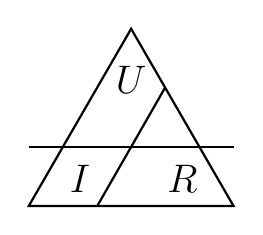
\begin{tikzpicture}[scale=1]
\draw[thick] (0,0) -- (2.6,0) -- (1.3,2.25) -- cycle;
\draw[thick] (0,0.75) -- (2.6,0.75);
\draw[thick] (0.87,0) -- (1.73,1.5);
\node at (1.3,1.6) {\Large $U$};
\node at (0.65,0.35) {\Large $I$};
\node at (1.95,0.35) {\Large $R$};
\end{tikzpicture}
\end{center}

The classic memory triangle above encodes all three rearrangements: cover
the quantity you want to find, and the remaining two show whether to
multiply or divide. Covering $U$ leaves $I$ beside $R$ (multiply, $U=IR$);
covering $I$ leaves $U$ over $R$ (divide, $I=U/R$); covering $R$ leaves
$U$ over $I$ (divide, $R=U/I$).

\begin{center}
\begin{tabular}{@{}llll@{}}
\toprule
Quantity & Symbol & Unit & Symbol for Unit \\
\midrule
Voltage (potential difference) & $U$ & volt & V \\
Current & $I$ & ampere & A \\
Resistance & $R$ & ohm & $\Omega$ \\
\bottomrule
\end{tabular}
\end{center}

\begin{examplebox}[Applying Ohm's law]
A 12\,V battery is connected across a 470\,$\Omega$ resistor. Find the
current.

\emph{Solution.}
\[
I = \frac{U}{R} = \frac{12\,\text{V}}{470\,\Omega} = 0.0255\,\text{A} = 25.5\,\text{mA}.
\]
\end{examplebox}

\begin{examtip}
Ohm's law questions on exams almost always require a prefix conversion as
part of the arithmetic (mA, k$\Omega$, etc.). Convert everything to base
units (V, A, $\Omega$) first, solve, then convert the final answer to a
sensible prefix.
\end{examtip}

\section{Electrical Power}

\textbf{Power} is the rate of doing work (transferring energy), measured
in \textbf{watts (W)}:
\[
P = \frac{W}{t}.
\]
In a DC circuit, electrical power delivered to a component is
\[
\boxed{P = UI}
\]
Combining this with Ohm's law gives two further useful forms, used
whenever voltage or current (rather than both) is known:
\[
P = I^{2}R, \qquad P = \frac{U^{2}}{R}.
\]

\begin{examplebox}[Power dissipation]
The 470\,$\Omega$ resistor from the previous example carries 25.5\,mA.
How much power does it dissipate, and could a standard $\tfrac{1}{4}$-W
resistor be used safely?

\emph{Solution.}
\[
P = I^2 R = (0.0255\,\text{A})^2 \times 470\,\Omega \approx 0.306\,\text{W}.
\]
This exceeds a $\tfrac{1}{4}$-W (0.25\,W) resistor's rating, so a
$\tfrac{1}{2}$-W or larger resistor should be used, ideally with margin
for safety (Section~\ref{sec:power-derating}).
\end{examplebox}

\begin{safetynote}[Power rating margin]
Never operate a resistor, or any dissipative component, right at its
rated maximum. A common engineering rule of thumb is to keep steady-state
dissipation below 50\% of the component's rating, both because
resistance itself drifts with temperature and because localized hot spots
can exceed the average calculated value.
\label{sec:power-derating}
\end{safetynote}

\section{Energy}

Energy is power sustained over time:
\[
W = Pt.
\]
When $P$ is in watts and $t$ is in seconds, $W$ comes out in joules.
Utility bills and battery capacities, however, are usually expressed in
\textbf{watt-hours (Wh)} or \textbf{kilowatt-hours (kWh)}, where $t$ is in
hours instead of seconds; $1\,\text{kWh} = 3.6\times10^{6}\,\text{J}$.
Battery amp-hour ratings, covered in Chapter~\ref{ch:power-sources}, use
the same underlying idea applied to charge instead of energy.

\section{Conductors, Insulators, and Semiconductors}

Materials are broadly classed by how easily their electrons can move
under an applied field:

\begin{itemize}
\item \textbf{Conductors} (copper, aluminum, silver, gold) have a ``sea''
of loosely bound valence electrons that move freely, giving very low
resistivity ($\rho \sim 10^{-8}\,\Omega\cdot\text{m}$). Used for wire,
antenna elements, PCB traces.
\item \textbf{Insulators} (PVC, ceramic, glass, air under normal
conditions) have tightly bound electrons and extremely high resistivity
($\rho \sim 10^{9}$--$10^{16}\,\Omega\cdot\text{m}$). Used to prevent
unwanted current paths --- wire jacketing, standoff insulators, capacitor
dielectrics.
\item \textbf{Semiconductors} (silicon, germanium) have resistivity
between the two, and --- crucially --- that resistivity can be controlled
by doping, temperature, or an applied field. This tunability is what
makes diodes, transistors, and integrated circuits possible
(Chapter~\ref{ch:semiconductors}).
\end{itemize}

\begin{quickreview}
\item Current $I = Q/t$; voltage $U = W/Q$; resistance $R = U/I$ (Ohm's
law, $U = IR$).
\item Conventional current flows from $+$ to $-$ through the external
circuit, opposite to actual electron drift.
\item $R = \rho \ell / A$: resistance rises with length, falls with
cross-sectional area, and depends on material resistivity.
\item Power: $P = UI = I^2R = U^2/R$; energy $W = Pt$.
\item Conductors, insulators, and semiconductors are distinguished by
resistivity and by whether that resistivity can be externally controlled.
\end{quickreview}

\begin{practiceproblems}
\item A 9\,V battery drives 300\,mA through a resistor. Find the
resistance.
\item Find the power dissipated by a 100\,$\Omega$ resistor carrying
50\,mA.
\item A device draws 2\,A at 13.8\,V for 3 hours. How much energy, in
watt-hours, did it consume?
\item A wire's length is doubled and its cross-sectional area is halved.
By what factor does its resistance change?
\item Explain, using the concept of resistivity, why thick antenna
feedline conductors have less loss than thin ones of the same length.
\end{practiceproblems}

\chapter{DC Circuits and the Resistor Color Code}
\label{ch:dc-circuits}

\section{Series Circuits}

Components are in \textbf{series} when they are connected end-to-end so
that the same current flows through each of them in turn, with no
alternate path.

\begin{center}
\begin{circuitikz}[scale=1]
\draw (0,0) to[battery1, l=$U$] (0,2)
      to[R, l=$R_1$] (2.5,2)
      to[R, l=$R_2$] (5,2)
      to[R, l=$R_3$] (5,0)
      -- (0,0);
\end{circuitikz}
\end{center}

\begin{keyidea}[Series circuit rules]
\begin{itemize}
\item Current is the \emph{same} through every component: $I_1 = I_2 = I_3 = I$.
\item Voltages \emph{add} to equal the source voltage:
$U = U_1 + U_2 + U_3$.
\item Resistances \emph{add}: $R_{\text{total}} = R_1 + R_2 + R_3 + \cdots$
\end{itemize}
\end{keyidea}

Because the same current flows through every series resistor, and
$U_n = IR_n$ for each one, the voltage across any single resistor in a
series chain is a fraction of the source voltage proportional to that
resistor's share of the total resistance --- the \textbf{voltage divider}
rule:
\[
U_n = U \times \frac{R_n}{R_{\text{total}}}.
\]

\begin{examplebox}[Voltage divider]
A 12\,V source drives a series circuit of $R_1 = 1\,\text{k}\Omega$ and
$R_2 = 3\,\text{k}\Omega$. Find the voltage across $R_2$.

\emph{Solution.} $R_{\text{total}} = 4\,\text{k}\Omega$, so
\[
U_2 = 12\,\text{V} \times \frac{3\,\text{k}\Omega}{4\,\text{k}\Omega} = 9\,\text{V}.
\]
\end{examplebox}

\section{Parallel Circuits}

Components are in \textbf{parallel} when they share the same pair of
nodes, so the same voltage appears across each of them.

\begin{center}
\begin{circuitikz}[scale=1]
\draw (0,0) to[battery1, l=$U$] (0,2.5) -- (1,2.5);
\draw (1,2.5) to[R, l=$R_1$] (1,0) -- (0,0);
\draw (1,2.5) -- (2.5,2.5) to[R, l=$R_2$] (2.5,0) -- (1,0);
\draw (2.5,2.5) -- (4,2.5) to[R, l=$R_3$] (4,0) -- (2.5,0);
\end{circuitikz}
\end{center}

\begin{keyidea}[Parallel circuit rules]
\begin{itemize}
\item Voltage is the \emph{same} across every branch: $U_1 = U_2 = U_3 = U$.
\item Currents \emph{add} to equal the total supplied current:
$I = I_1 + I_2 + I_3$.
\item Conductances add, so resistances combine by the reciprocal rule:
\[
\frac{1}{R_{\text{total}}} = \frac{1}{R_1} + \frac{1}{R_2} + \frac{1}{R_3} + \cdots
\]
\end{itemize}
\end{keyidea}

For exactly two resistors in parallel, this simplifies to the frequently
used \textbf{product-over-sum} shortcut:
\[
R_{\text{total}} = \frac{R_1 R_2}{R_1 + R_2}.
\]
A useful sanity check: the parallel combination of any set of resistors is
always \emph{smaller} than the smallest individual resistor, because
adding a parallel path always gives current an easier route.

\begin{examplebox}[Parallel resistance]
Find the total resistance of a 100\,$\Omega$ and a 150\,$\Omega$ resistor
in parallel.

\emph{Solution.}
\[
R_{\text{total}} = \frac{100 \times 150}{100 + 150} = \frac{15000}{250} = 60\,\Omega.
\]
Notice this is less than 100\,$\Omega$, the smaller of the two, as expected.
\end{examplebox}

Currents split between parallel branches in inverse proportion to
resistance (the \textbf{current divider} rule); for two resistors,
\[
I_1 = I_{\text{total}} \times \frac{R_2}{R_1+R_2}, \qquad
I_2 = I_{\text{total}} \times \frac{R_1}{R_1+R_2}.
\]

\section{Series--Parallel Combinations}

Real circuits usually combine both arrangements. The systematic method is
to redraw the circuit in stages: identify a sub-group of resistors that
are purely in series or purely in parallel, collapse that sub-group into
a single equivalent resistor, and repeat until only one resistor remains.
Work from the ``furthest'' part of the circuit from the source inward.

\begin{examplebox}[Series--parallel reduction]
$R_1 = 2\,\text{k}\Omega$ is in series with the parallel combination of
$R_2 = 4\,\text{k}\Omega$ and $R_3 = 4\,\text{k}\Omega$, all driven by a
10\,V source. Find the total current drawn from the source.

\emph{Solution.} First collapse the parallel pair:
$R_{23} = (4\times4)/(4+4) = 2\,\text{k}\Omega$. This is now in series
with $R_1$: $R_{\text{total}} = 2 + 2 = 4\,\text{k}\Omega$. Then
$I = U/R_{\text{total}} = 10\,\text{V}/4\,\text{k}\Omega = 2.5\,\text{mA}$.
\end{examplebox}

\section{Kirchhoff's Laws}

The series and parallel rules above are special cases of two more general
laws, published by Gustav Kirchhoff in 1845, which apply to \emph{any}
circuit topology, no matter how tangled.

\begin{keyidea}[Kirchhoff's Current Law (KCL)]
The sum of currents entering a node equals the sum of currents leaving it
--- charge cannot accumulate at a node in steady state:
\[
\sum I_{\text{in}} = \sum I_{\text{out}}.
\]
\end{keyidea}

\begin{keyidea}[Kirchhoff's Voltage Law (KVL)]
The sum of voltage rises and drops around any closed loop is zero ---
energy gained from sources in a loop equals energy dissipated by
components in that loop:
\[
\sum U_{\text{loop}} = 0.
\]
\end{keyidea}

KCL and KVL are the foundation of general circuit analysis techniques
(mesh and nodal analysis) taught in full electrical-engineering courses;
for amateur radio purposes, it is enough to recognize that the series and
parallel rules of this chapter are direct consequences of these two laws,
and to be able to apply KVL/KCL qualitatively --- for example, to
recognize that the voltage across a shorted component must be zero, or
that current from a source must ultimately return to that source.

\section{Superposition and Thévenin Equivalents (Brief Introduction)}

Two further techniques appear in more advanced treatments and occasionally
in advanced-class exams:

\begin{itemize}
\item \textbf{Superposition}: in a linear circuit with multiple sources,
the response (current or voltage) at any point equals the sum of the
responses caused by each source acting alone, with all other independent
voltage sources replaced by short circuits and all other independent
current sources replaced by open circuits.
\item \textbf{Thévenin's theorem}: any two-terminal network of linear
sources and resistors can be replaced, from the point of view of an
external load, by a single equivalent voltage source $U_{\text{Th}}$ in
series with a single equivalent resistance $R_{\text{Th}}$. This is
extremely useful for analyzing how a source (such as a transmitter's
final amplifier) will drive different loads, and reappears in
Chapter~\ref{ch:transmission-lines} when discussing impedance matching.
\end{itemize}

\section{The Resistor Color Code}
\label{sec:color-code}

Small fixed resistors are usually too small to print numeric values on,
so their value and tolerance are encoded as a sequence of colored bands.
The most common scheme uses four bands: two significant digits, a
multiplier, and a tolerance.

\begin{center}
\renewcommand{\arraystretch}{1.15}
\begin{tabular}{@{}lccc@{}}
\toprule
Color & Digit & Multiplier & Tolerance \\
\midrule
\cellcolor{black!85}\textcolor{white}{Black} & 0 & $\times 10^{0}$ & --- \\
\cellcolor{brown!70!black}\textcolor{white}{Brown} & 1 & $\times 10^{1}$ & $\pm 1\%$ \\
\cellcolor{red}Red & 2 & $\times 10^{2}$ & $\pm 2\%$ \\
\cellcolor{orange}Orange & 3 & $\times 10^{3}$ & --- \\
\cellcolor{yellow}Yellow & 4 & $\times 10^{4}$ & --- \\
\cellcolor{green!70!black}\textcolor{white}{Green} & 5 & $\times 10^{5}$ & $\pm 0.5\%$ \\
\cellcolor{blue}\textcolor{white}{Blue} & 6 & $\times 10^{6}$ & $\pm 0.25\%$ \\
\cellcolor{violet}\textcolor{white}{Violet} & 7 & $\times 10^{7}$ & $\pm 0.1\%$ \\
\cellcolor{gray!60}Grey & 8 & $\times 10^{8}$ & --- \\
White & 9 & $\times 10^{9}$ & --- \\
\cellcolor{yellow!70!orange}Gold & --- & $\times 10^{-1}$ & $\pm 5\%$ \\
\cellcolor{gray!30}Silver & --- & $\times 10^{-2}$ & $\pm 10\%$ \\
None & --- & --- & $\pm 20\%$ \\
\bottomrule
\end{tabular}
\end{center}

For a \textbf{4-band resistor}, read bands 1--2 as significant digits,
band 3 as the power-of-ten multiplier, and band 4 as tolerance:
\[
\text{Value} = (\text{digit}_1 \, \text{digit}_2) \times 10^{\text{multiplier}} \,\Omega.
\]
A \textbf{5-band resistor} (more common for precision, $\pm1\%$ or
better, resistors) uses three significant digits before the multiplier
band.

\begin{examplebox}[Reading the color code]
A resistor shows the bands Brown, Black, Red, Gold. Find its value and
tolerance.

\emph{Solution.} Brown = 1, Black = 0, so the significant digits are
``10.'' Red is the multiplier, $\times10^2 = \times100$. So
$R = 10 \times 100 = 1000\,\Omega = 1\,\text{k}\Omega$. Gold indicates
$\pm5\%$ tolerance, so the resistor's true value lies between 950\,$\Omega$
and 1050\,$\Omega$.
\end{examplebox}

\begin{examtip}
A popular mnemonic for the digit sequence 0--9 (Black, Brown, Red,
Orange, Yellow, Green, Blue, Violet, Grey, White) is: \emph{``B}ad
\emph{B}oys \emph{R}ob \emph{O}ur \emph{Y}oung \emph{G}irls \emph{B}ut
\emph{V}iolet \emph{G}ives \emph{W}illingly.'' Use whichever mnemonic
sticks; what matters on an exam is speed and accuracy, not elegance.
\end{examtip}

\section{Preferred Values (E-series)}

Resistors (and capacitors) are not manufactured at every possible value;
they follow standardized \textbf{preferred value} series (E6, E12, E24,
E96, \dots) where the number indicates how many values are spaced
per decade. The E12 series, for instance, uses twelve values per decade
spaced so that the maximum error between any achievable value and a
desired value, given the series tolerance, stays small:
\[
1.0,\ 1.2,\ 1.5,\ 1.8,\ 2.2,\ 2.7,\ 3.3,\ 3.9,\ 4.7,\ 5.6,\ 6.8,\ 8.2 \ (\times 10^{n}).
\]
This is why component catalogs list ``4.7\,k$\Omega$'' and
``5.6\,k$\Omega$'' resistors but not ``5.0\,k$\Omega$'' --- the nearest
E12 values are used instead, and circuit designs are built around
whatever the nearest standard value achieves.

\begin{quickreview}
\item Series: same current, voltages add, resistances add.
\item Parallel: same voltage, currents add, resistances combine by
reciprocal sum (or product-over-sum for two resistors).
\item Kirchhoff's Current Law and Voltage Law are the general principles
underlying the series/parallel shortcuts.
\item Resistor color bands encode two or three significant digits, a
multiplier, and a tolerance.
\item Component values follow standardized E-series preferred value
tables, not arbitrary round numbers.
\end{quickreview}

\begin{practiceproblems}
\item Three resistors, 100\,$\Omega$, 220\,$\Omega$, and 330\,$\Omega$,
are in series across a 9\,V battery. Find the total resistance, the
current, and the voltage across the 220\,$\Omega$ resistor.
\item Find the equivalent resistance of 470\,$\Omega$, 470\,$\Omega$, and
1\,k$\Omega$ in parallel.
\item A resistor's bands read Yellow, Violet, Orange, Gold. Find its
value and tolerance range.
\item Explain, using KCL, why the total current entering a series--parallel
network must equal the current leaving it, even though internal branch
currents differ.
\item Two 100\,$\Omega$ resistors and one 220\,$\Omega$ resistor are
connected so that the 220\,$\Omega$ is in series with the parallel
combination of the two 100\,$\Omega$ units, across a 15\,V source. Find
the total current.
\end{practiceproblems}

\chapter{Electric, Magnetic, and Electromagnetic Fields}
\label{ch:fields}

Everything a radio does --- store energy in a capacitor, store energy in
an inductor, radiate a signal from an antenna, propagate that signal
across an ocean --- is a manifestation of electric and magnetic fields.
This chapter builds the field concepts needed to understand components
(Part~II) and antennas and propagation (Part~IV).

\section{The Electric Field}

An \textbf{electric field} exists in the region around any electric
charge; it is defined as the force per unit charge that a small positive
``test charge'' would experience at a given point:
\[
E = \frac{F}{q} \qquad [\text{volts per metre, V/m}]
\]
Field lines point away from positive charges and toward negative charges.
Between two flat, oppositely charged parallel plates separated by
distance $d$ with potential difference $U$ between them, the field is
uniform and given by
\[
E = \frac{U}{d}.
\]
This is precisely the geometry inside a parallel-plate capacitor
(Chapter~\ref{ch:capacitors}): a capacitor is, at its core, a device for
storing energy in an electric field confined between two conductors.

\begin{keyidea}
The electric field describes how strongly a charge distribution can push
or pull on other charges. It is the mechanism by which a capacitor stores
energy and by which a transmitting antenna's near field couples to
nearby objects.
\end{keyidea}

\section{The Magnetic Field}

A \textbf{magnetic field} is produced by moving charge (current) and is
described by the flux density $B$, measured in \textbf{tesla (T)}. Unlike
electric field lines, magnetic field lines have no starting or ending
point; they form closed loops. For a long, straight conductor carrying
current $I$, the field at perpendicular distance $r$ is
\[
B = \frac{\mu_0 I}{2\pi r}
\]
where $\mu_0 = 4\pi \times 10^{-7}\,\text{H/m}$ is the \textbf{permeability
of free space}. The direction of the field circles the conductor
according to the \textbf{right-hand rule}: point the thumb of your right
hand in the direction of conventional current flow, and your fingers curl
in the direction of the magnetic field.

Winding a conductor into a coil concentrates and reinforces this field
inside the loops, which is precisely how an \textbf{inductor}
(Chapter~\ref{ch:inductors}) stores energy in a magnetic field, and how a
loop antenna couples to the magnetic component of a radio wave.

\begin{center}
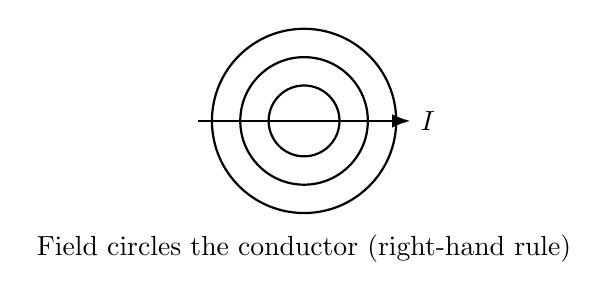
\begin{tikzpicture}[scale=0.9]
\draw[thick,-{Latex}] (0,0) -- (3,0) node[right] {$I$};
\foreach \r in {0.5,0.9,1.3}{
  \draw[thick,-{Latex}] (1.5,0) circle (\r);
}
\node at (1.5,-1.8) {Field circles the conductor (right-hand rule)};
\end{tikzpicture}
\end{center}

\section{Magnetic Flux and Faraday's Law}

\textbf{Magnetic flux}, $\Phi$, measured in \textbf{webers (Wb)}, is the
total magnetic field passing through a given area:
\[
\Phi = B \cdot A
\]
for a uniform field $B$ perpendicular to area $A$. \textbf{Faraday's law of
induction} states that a changing magnetic flux through a loop induces an
EMF around that loop:
\[
\mathcal{E} = -N\frac{d\Phi}{dt}
\]
where $N$ is the number of turns of the loop and the negative sign (Lenz's
law) indicates that the induced EMF always opposes the change that
created it. Faraday's law is the working principle behind
\textbf{inductors} (an inductor opposes changes in current because that
current change causes a changing flux, which induces an opposing EMF),
\textbf{transformers} (Chapter~\ref{ch:transformers}), and the reception
of radio signals by any loop or wire antenna.

\begin{keyidea}[Lenz's law, intuitively]
An induced current always flows in the direction that opposes the change
that produced it. This is why inductors resist sudden changes in
current, and why energy must be supplied to overcome this opposition when
current is increased or decreased quickly.
\end{keyidea}

\section{The Electromagnetic Field and Maxwell's Insight}

Electric and magnetic fields are not independent phenomena; they are two
aspects of a single \textbf{electromagnetic field}. James Clerk Maxwell
showed in the 1860s, through four coupled equations now called
\textbf{Maxwell's equations}, that:

\begin{itemize}
\item A changing electric field produces a magnetic field (this
completes the symmetry of Faraday's law, and was Maxwell's key
addition --- the ``displacement current'' term).
\item A changing magnetic field produces an electric field (Faraday's
law).
\end{itemize}

These two facts together mean that, once created, a time-varying
electric field and a time-varying magnetic field can regenerate each
other indefinitely, propagating outward from their source as a
self-sustaining wave --- an \textbf{electromagnetic wave} --- without
needing a material medium to carry them. Maxwell calculated the
predicted speed of such a wave from purely electrical and magnetic
constants,
\[
c = \frac{1}{\sqrt{\mu_0 \varepsilon_0}} \approx 2.998 \times 10^{8}\,\text{m/s},
\]
and found it matched the already-measured speed of light --- correctly
concluding that light itself is an electromagnetic wave. Radio waves,
microwaves, infrared, visible light, ultraviolet, X-rays, and gamma rays
are all electromagnetic waves, differing only in frequency (and hence
wavelength); amateur radio operates in the radio-frequency portion of
this same spectrum.

\section{Properties of a Traveling EM Wave}

In a radio wave traveling through free space, the electric field $E$ and
magnetic field $H$ oscillate perpendicular to each other and to the
direction of propagation, in phase, with a fixed ratio between them (the
\textbf{impedance of free space}, $Z_0 = \sqrt{\mu_0/\varepsilon_0}
\approx 377\,\Omega$).

\begin{center}
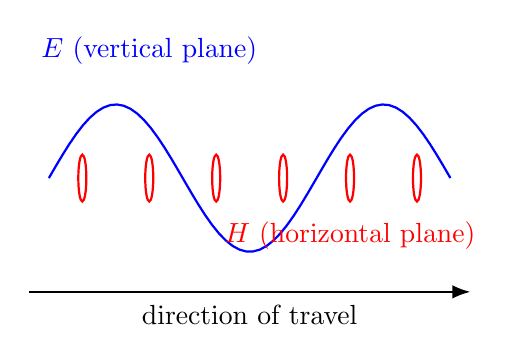
\begin{tikzpicture}[scale=0.85]
\draw[thick,blue,domain=0:6,samples=60] plot ({\x},{1.1*sin(\x*90)});
\node[blue,anchor=south] at (1.5,1.55) {$E$ (vertical plane)};
\foreach \x in {0.5,1.5,2.5,3.5,4.5,5.5}{
  \draw[thick,red] (\x,0) ellipse (0.06 and 0.35);
}
\node[red,anchor=north] at (4.5,-0.5) {$H$ (horizontal plane)};
\draw[-{Latex},thick] (-0.3,-1.7) -- (6.3,-1.7);
\node[anchor=north] at (3,-1.75) {direction of travel};
\end{tikzpicture}
\end{center}

The \textbf{wavelength} $\lambda$, \textbf{frequency} $f$, and
\textbf{speed of light} $c$ are related by
\[
\boxed{c = f\lambda} \qquad \Longrightarrow \qquad \lambda = \frac{c}{f}, \quad f = \frac{c}{\lambda}.
\]
This single relationship is one of the most exam-relevant formulas in the
entire book: it converts between the two ways radio frequencies are
described (as a frequency in Hz, or as a wavelength in metres, as in
``the 20-metre band'') and underlies antenna dimension calculations in
Chapter~\ref{ch:antennas}.

\begin{examplebox}[Frequency--wavelength conversion]
Find the wavelength corresponding to 14.200\,MHz.

\emph{Solution.}
\[
\lambda = \frac{c}{f} = \frac{2.998\times10^{8}\,\text{m/s}}{14.200\times10^{6}\,\text{Hz}} \approx 21.1\,\text{m}.
\]
This is why 14\,MHz is colloquially called ``the 20\,m band'' --- 21.1\,m
rounds, by amateur radio band-naming convention, to the nearest
traditional metre-band label.
\end{examplebox}

\section{Polarization}

The \textbf{polarization} of an EM wave describes the orientation of its
electric field vector. If $E$ stays in a fixed plane as the wave travels
(e.g., always vertical, or always horizontal), the wave is
\textbf{linearly polarized}; a horizontal dipole radiates a horizontally
polarized wave, a vertical antenna radiates a vertically polarized wave.
If the $E$ field instead rotates as the wave travels, tracing a helix, the
wave is \textbf{circularly} (or, more generally, \textbf{elliptically})
polarized --- used heavily in satellite work, where a spacecraft's
orientation relative to a ground station is constantly changing, so
neither pure horizontal nor pure vertical polarization stays aligned.
Polarization mismatch between a transmitting and receiving antenna causes
signal loss (Chapter~\ref{ch:antennas}), which is why matching
polarization matters when choosing or orienting an antenna.

\begin{quickreview}
\item Electric field $E = F/q$ (V/m); magnetic flux density $B$ (tesla);
flux $\Phi = BA$ (weber).
\item Faraday's law: a changing flux induces an EMF, $\mathcal{E} =
-N\,d\Phi/dt$; Lenz's law fixes the sign (opposition to change).
\item Maxwell's equations show that changing $E$ and $B$ fields sustain
each other, propagating as an electromagnetic wave at $c \approx
3\times10^{8}\,\text{m/s}$.
\item $c = f\lambda$ links frequency and wavelength --- essential for
antenna design and band naming.
\item Polarization describes the orientation of the wave's electric
field; mismatched polarization causes signal loss.
\end{quickreview}

\begin{practiceproblems}
\item Find the magnetic field 5\,cm from a straight wire carrying 2\,A.
\item A single-turn loop of area 0.01\,m$^2$ experiences a flux change
from 0 to 5\,mWb in 0.1\,s. Find the induced EMF.
\item Calculate the wavelength for 145.500\,MHz and for 433.500\,MHz;
identify the traditional amateur band name for each.
\item Explain, in terms of Maxwell's equations, why a radio wave can
cross the vacuum of space with no medium to carry it, unlike a sound
wave.
\item A satellite station uses circular polarization while a fixed home
station uses a horizontal linear-polarized antenna. Explain qualitatively
why using circular polarization at both ends often improves the link.
\end{practiceproblems}

\chapter{Alternating Current and Sinusoidal Signals}
\label{ch:ac-theory}

Every radio signal is an alternating current (AC) waveform. This chapter
develops the mathematics of sinusoidal AC --- amplitude, frequency,
phase, and the RMS value --- that underlies every later chapter on
reactance, resonance, and modulation.

\section{Direct Current vs.\ Alternating Current}

\textbf{Direct current (DC)} flows in one direction only in a circuit;
its magnitude may be constant (a battery) or may vary, but its polarity
does not reverse. \textbf{Alternating current (AC)} periodically reverses
direction. The most important AC waveform, both because it is
mathematically fundamental and because it is what oscillators naturally
produce, is the \textbf{sine wave}.

\section{Describing a Sine Wave}

A sinusoidal voltage varying with time $t$ is written
\[
\boxed{v(t) = V_{\text{pk}}\sin(\omega t + \phi)}
\]
where:
\begin{itemize}
\item $V_{\text{pk}}$ is the \textbf{peak amplitude} (maximum
instantaneous value), in volts.
\item $\omega = 2\pi f$ is the \textbf{angular frequency}, in radians per
second, where $f$ is the frequency in hertz.
\item $\phi$ is the \textbf{phase angle}, describing a time offset
relative to a reference, in radians or degrees.
\end{itemize}

\begin{center}
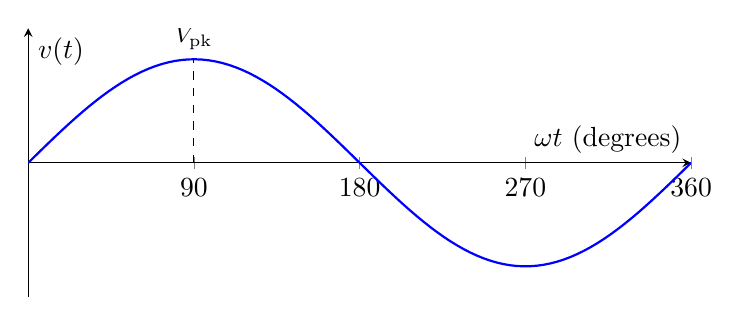
\begin{tikzpicture}[scale=1]
\begin{axis}[
  width=10cm, height=5cm,
  xlabel={$\omega t$ (degrees)}, ylabel={$v(t)$},
  xmin=0, xmax=360, ymin=-1.3, ymax=1.3,
  xtick={0,90,180,270,360}, ytick=\empty,
  axis lines=middle, samples=100,
  domain=0:360,
  enlargelimits=false
]
\addplot[thick,blue] {sin(x)};
\draw[dashed] (axis cs:90,0) -- (axis cs:90,1) node[above] {\footnotesize $V_{\text{pk}}$};
\end{axis}
\end{tikzpicture}
\end{center}

\subsection{Period and Frequency}

The \textbf{period} $T$ is the time for one complete cycle; frequency is
its reciprocal:
\[
\boxed{f = \frac{1}{T}} \qquad [\text{hertz, Hz} = \text{cycles per second}]
\]
A 14\,MHz signal completes $14\times10^{6}$ cycles every second, so its
period is $T = 1/(14\times10^{6}) \approx 71.4\,\text{ns}$.

\subsection{Amplitude Measures}

A sine wave can be described by several different amplitude measures,
and confusing them is one of the most common sources of error in AC
calculations:

\begin{center}
\begin{tabular}{@{}lll@{}}
\toprule
Measure & Meaning & Relation to $V_{\text{pk}}$ \\
\midrule
Peak ($V_{\text{pk}}$) & Maximum instantaneous value & --- \\
Peak-to-peak ($V_{\text{pp}}$) & Total swing, trough to crest & $V_{\text{pp}} = 2V_{\text{pk}}$ \\
RMS ($V_{\text{rms}}$) & Effective (heating) value & $V_{\text{rms}} = V_{\text{pk}}/\sqrt{2}$ \\
Average ($V_{\text{avg}}$) & Mean of the rectified waveform & $V_{\text{avg}} = 2V_{\text{pk}}/\pi$ \\
\bottomrule
\end{tabular}
\end{center}

\begin{keyidea}[Why RMS matters]
The \textbf{root-mean-square (RMS)} value of an AC waveform is defined so
that it produces the \emph{same heating effect} (the same average power
dissipation in a resistor) as a DC voltage of the same numerical value.
All of the DC power formulas from Chapter~\ref{ch:electricity}
($P=UI$, $P=I^2R$, $P=U^2/R$) apply directly to AC \emph{if} RMS values
are used for $U$ and $I$. Unless stated otherwise, voltages and currents
quoted for AC mains, transmitter output, and test equipment readings are
always RMS values.
\end{keyidea}

For a pure sine wave, $V_{\text{rms}} = V_{\text{pk}}/\sqrt{2} \approx
0.707\,V_{\text{pk}}$. This factor of $1/\sqrt2$ comes from averaging
$\sin^2(\theta)$ over a full cycle, which equals $\tfrac12$.

\begin{examplebox}[RMS conversion]
A sine wave has a peak voltage of 325\,V (typical of 230\,V AC mains).
Find its RMS value.

\emph{Solution.}
\[
V_{\text{rms}} = \frac{V_{\text{pk}}}{\sqrt2} = \frac{325}{1.414} \approx 230\,\text{V}.
\]
This confirms that ``230\,V mains'' is quoted as an RMS value.
\end{examplebox}

\section{Phase}

\textbf{Phase} describes the timing relationship between two waveforms of
the same frequency. Two sine waves are \textbf{in phase} if their peaks
and zero-crossings line up exactly ($\phi = 0$); they are \textbf{out of
phase} by however many degrees (or radians) one is shifted relative to
the other. A phase difference of $90\degree$ is described as
\textbf{quadrature}; $180\degree$ means the waveforms are exact mirror
images of each other (in \textbf{antiphase}).

Phase becomes critical once reactive components are introduced
(Chapters~\ref{ch:capacitors}--\ref{ch:rlc-resonance}): unlike a
resistor, a capacitor or inductor shifts the phase between the voltage
across it and the current through it, which is the origin of
\textbf{reactance} and \textbf{impedance}.

\section{The Rotating Phasor Picture}

A sine wave can be visualized as the vertical projection of a vector (a
\textbf{phasor}) of length $V_{\text{pk}}$ rotating counterclockwise at
angular velocity $\omega$. This picture --- formalized using complex
numbers as $V_{\text{pk}}e^{j(\omega t + \phi)}$ --- turns AC circuit
analysis into algebra: instead of tracking a continuously varying
instantaneous voltage, engineers track a fixed complex number (magnitude
and phase) per frequency, and the differential-equation relationships
between voltage and current across capacitors and inductors become
simple multiplication by a complex impedance. This is the ``$j$''
notation used throughout Chapters~\ref{ch:capacitors}--\ref{ch:rlc-resonance}.

\section{Why Sine Waves Are Special}

Sine waves are the natural output of resonant physical systems (a
pendulum, a vibrating string, an LC oscillator) and, crucially, are the
\emph{only} waveform shape that a linear circuit (one built from
resistors, capacitors, and inductors) cannot distort --- passing a sine
wave through a linear filter changes its amplitude and phase but never
its fundamental shape. This property, combined with the mathematical fact
that \emph{any} periodic waveform can be built from a sum of sine waves
at different frequencies (Fourier's theorem, Chapter~\ref{ch:non-sine}),
is why sinusoidal analysis is the foundation for understanding every
other waveform used in radio.

\begin{quickreview}
\item $v(t) = V_{\text{pk}}\sin(\omega t + \phi)$, with $\omega = 2\pi f$
and $f = 1/T$.
\item $V_{\text{pp}} = 2V_{\text{pk}}$; $V_{\text{rms}} =
V_{\text{pk}}/\sqrt2 \approx 0.707 V_{\text{pk}}$; DC power formulas apply
to AC when RMS values are used.
\item Phase describes timing offset between waveforms; $90\degree$ is
quadrature, $180\degree$ is antiphase.
\item The rotating phasor (complex-exponential) picture turns AC analysis
into algebra with complex numbers.
\item Any periodic waveform is a sum of sine waves at different
frequencies (previewing Fourier analysis, Chapter~\ref{ch:non-sine}).
\end{quickreview}

\begin{practiceproblems}
\item A sine wave has $V_{\text{rms}} = 120\,\text{V}$. Find
$V_{\text{pk}}$ and $V_{\text{pp}}$.
\item Find the period of a 7.100\,MHz signal.
\item Two sine waves of the same frequency have a phase difference of
$90\degree$. What term describes this relationship?
\item A signal generator is set to 1\,kHz with a peak amplitude of 5\,V.
Write the instantaneous voltage $v(t)$ as an equation, assuming zero
phase offset.
\item Explain why AC voltmeters are calibrated to read RMS rather than
peak values.
\end{practiceproblems}

\chapter{Non-Sinusoidal Signals and Fourier Analysis}
\label{ch:non-sine}

Not every useful waveform is a sine wave. Square waves clock digital
logic, sawtooth waves sweep oscilloscopes and older TV displays, and the
keyed on/off waveform of Morse code is about as far from a sine wave as a
signal can get. This chapter explains how such waveforms relate back to
the sinusoidal theory of Chapter~\ref{ch:ac-theory}, and why that
relationship matters for bandwidth and interference.

\section{Common Non-Sinusoidal Waveforms}

\begin{figure}[H]
\centering
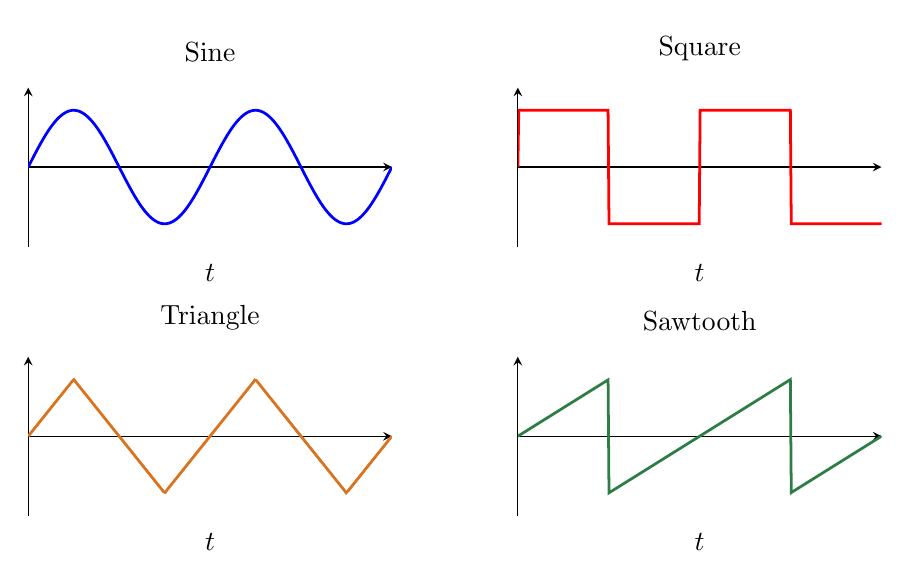
\begin{tikzpicture}
\begin{groupplot}[
  group style={group size=2 by 2, horizontal sep=1.6cm, vertical sep=1.4cm},
  width=6.2cm, height=3.6cm, axis lines=middle,
  xtick=\empty, ytick=\empty, ymin=-1.4, ymax=1.4, xmin=0, xmax=4,
  domain=0:4, samples=200,
  every axis plot/.append style={line width=1pt},
  every axis x label/.style={at={(axis description cs:0.5,-0.05)},anchor=north},
]
\nextgroupplot[title={Sine},xlabel={$t$}]
\addplot[blue] {sin(x*180)};

\nextgroupplot[title={Square},xlabel={$t$}]
\addplot[red,samples=400,unbounded coords=jump] {sign(sin(x*180))};

\nextgroupplot[title={Triangle},xlabel={$t$}]
\addplot[rorange] {asin(sin(x*180))/90};

\nextgroupplot[title={Sawtooth},xlabel={$t$}]
\addplot[rgreenline,samples=400,unbounded coords=jump] {2*(x/2-floor(x/2+0.5))};
\end{groupplot}
\end{tikzpicture}
\caption{Common periodic waveforms: sine, square, triangle, and
sawtooth, each shown over several cycles.}
\label{fig:waveforms}
\end{figure}

\begin{itemize}
\item \textbf{Square wave}: switches abruptly between two levels, spending
equal time at each (50\% duty cycle). Produced by digital logic gates,
keyed CW (approximately), and switching-mode power supplies.
\item \textbf{Triangle wave}: rises and falls linearly at a constant
rate. Used in some function generators and as a building block for
sweep and ramp circuits.
\item \textbf{Sawtooth wave}: rises linearly then drops sharply (or vice
versa). Classic use: the horizontal deflection sweep in a
cathode-ray-tube display.
\item \textbf{Pulse train}: a waveform that is at one level for a short
time and at another level for the rest of the period, characterized by
its \textbf{duty cycle} (fraction of the period spent ``high''). Digital
data and radar are naturally pulse-like.
\end{itemize}

\section{Fourier's Theorem}
\label{sec:fourier}

The mathematician Joseph Fourier proved a result of enormous consequence
for radio engineering: \emph{any} periodic waveform, no matter its shape,
can be expressed as a sum (in general, an infinite sum) of sine and
cosine waves at the fundamental frequency and its integer multiples
(\textbf{harmonics}):
\[
x(t) = a_0 + \sum_{n=1}^{\infty} \left[a_n \cos(n\omega_0 t) + b_n \sin(n\omega_0 t)\right]
\]
where $\omega_0 = 2\pi f_0$ is the fundamental angular frequency and
$a_0, a_n, b_n$ are coefficients determined by the waveform's shape. This
means a waveform's \emph{shape} and its \emph{frequency content} are two
views of the same underlying signal, related by the \textbf{Fourier
transform} (for non-periodic or more general signals) or the
\textbf{Fourier series} (for periodic signals, as written above).

\begin{keyidea}
Every non-sinusoidal periodic signal occupies more than one frequency: a
fundamental plus a ladder of harmonics. A signal's bandwidth --- how much
of the radio spectrum it actually occupies --- is fundamentally a
statement about its Fourier content, not just its nominal ``frequency.''
\end{keyidea}

\subsection{Square Wave Harmonics}

A symmetric square wave of fundamental frequency $f_0$ and peak amplitude
$A$ contains \emph{only odd} harmonics, with amplitude falling off as
$1/n$:
\[
x(t) = \frac{4A}{\pi}\left[\sin(\omega_0 t) + \frac{1}{3}\sin(3\omega_0 t) + \frac{1}{5}\sin(5\omega_0 t) + \cdots\right]
\]
This is why a keyed CW signal or a switching power supply, even though it
is nominally operating at one frequency, actually radiates energy at that
frequency's odd multiples too --- a real-world source of harmonic
interference (Section~\ref{sec:harmonic-interference}) unless filtered.

\begin{examplebox}[Predicting a harmonic frequency]
A square-wave clock oscillates at 7.023\,MHz. At what frequency would you
expect to find its strongest spurious harmonic, and in which amateur band
might it fall?

\emph{Solution.} The strongest harmonic of a square wave (after the
fundamental) is the third harmonic: $3 \times 7.023 = 21.069\,\text{MHz}$,
which falls inside the 15\,m amateur band (21.000--21.450\,MHz in most
IARU Region 1/2/3 allocations) --- a classic real-world case for
low-pass filtering a keyed oscillator or transmitter output.
\end{examplebox}

\section{Bandwidth and Rise Time}

A perfectly square edge (instantaneous transition) requires
\emph{infinite} bandwidth to reproduce exactly, because it needs
harmonics out to $n \to \infty$ to build the sharp corner. Real circuits
have finite bandwidth, so real square waves always have a finite
\textbf{rise time} $t_r$ (time to transition, conventionally measured
from 10\% to 90\% of full amplitude). A useful rule of thumb links rise
time and the bandwidth $B$ needed to reproduce it reasonably faithfully:
\[
B \approx \frac{0.35}{t_r}.
\]
This relationship explains why fast-keyed digital or CW signals, or
poorly shaped keying waveforms, splatter energy into adjacent parts of
the band --- an important practical and courtesy consideration when
operating, and the reason well-designed transmitters deliberately shape
(``soften'') their keying edges.

\begin{safetynote}[Key clicks and splatter]
Overly fast keying transitions (``hard keying'') generate broadband
clicks that can interfere with stations operating hundreds of kilohertz
away. Modern transmitters shape the CW envelope with a short rise/fall
time (typically several milliseconds) specifically to keep the emitted
bandwidth narrow. This is both good operating practice and, in most
countries, a regulatory requirement on out-of-band emissions.
\label{sec:harmonic-interference}
\end{safetynote}

\section{DC Offset and the Mean Value}

The $a_0$ term in the Fourier series represents the waveform's
\textbf{DC component} --- its average value over a full cycle. A sine
wave that swings symmetrically about zero has $a_0 = 0$; a keyed pulse
train that is ``on'' more than it is ``off'' has a nonzero DC component
equal to (peak value) $\times$ (duty cycle). This matters practically
when a waveform passes through a transformer or capacitor-coupled stage,
neither of which passes a DC component --- the shape of the waveform will
change (its average will be forced back to zero) even though its AC
content is otherwise preserved.

\section{Spectral (Frequency-Domain) View}

Plotting a signal's amplitude at each frequency, rather than its
instantaneous value over time, gives its \textbf{spectrum} --- exactly
what a spectrum analyzer or waterfall display shows. A pure sine wave
appears as a single vertical line at its frequency; a square wave appears
as a line at the fundamental plus progressively smaller lines at each odd
harmonic; a burst of noise appears as energy spread continuously across a
range of frequencies. Learning to think in both the \textbf{time domain}
(a scope trace) and the \textbf{frequency domain} (a spectrum display)
simultaneously is one of the most valuable skills a radio amateur can
develop, and is essential for understanding modulation
(Chapter~\ref{ch:modulation}).

\begin{quickreview}
\item Any periodic waveform is a sum of sine/cosine harmonics of its
fundamental frequency (Fourier series).
\item A symmetric square wave contains only odd harmonics, falling off as
$1/n$ in amplitude.
\item Sharper edges (shorter rise time) require more bandwidth,
approximately $B \approx 0.35/t_r$.
\item A waveform's DC component is its Fourier $a_0$ term --- the
average value over one cycle.
\item Time-domain and frequency-domain views describe the same signal
from two complementary perspectives.
\end{quickreview}

\begin{practiceproblems}
\item List the first three nonzero harmonics (as multiples of $f_0$) of a
symmetric square wave.
\item A 3.573\,MHz CW oscillator's third harmonic falls near which
amateur band?
\item A digital keying circuit has a rise time of 1\,ms. Estimate the
bandwidth this implies, and comment on whether this is adequate for
narrow, splatter-free CW.
\item Explain why a capacitor-coupled audio stage will not faithfully
pass a waveform with a strong DC offset.
\item Sketch (in words) how the spectrum of a triangle wave would differ
from that of a square wave of the same fundamental frequency.
\end{practiceproblems}


\part{Passive Components and Circuits}
\chapter{Capacitors and Capacitive Reactance}
\label{ch:capacitors}

\section{The Capacitor}

A \textbf{capacitor} stores energy in an electric field between two
conductive plates separated by an insulating \textbf{dielectric}. Its
defining property is \textbf{capacitance} $C$, measured in
\textbf{farads (F)}:
\[
\boxed{C = \frac{Q}{U}}
\]
where $Q$ is the charge stored (coulombs) and $U$ is the voltage across
the plates. One farad is a very large unit; practical capacitors are
usually specified in microfarads ($\mu$F), nanofarads (nF), or
picofarads (pF).

For a simple parallel-plate capacitor with plate area $A$, separation
$d$, and a dielectric of permittivity $\varepsilon = \varepsilon_r
\varepsilon_0$,
\[
C = \frac{\varepsilon_r \varepsilon_0 A}{d}
\]
where $\varepsilon_0 = 8.854\times10^{-12}\,\text{F/m}$ is the
permittivity of free space and $\varepsilon_r$ is the dielectric's
\textbf{relative permittivity} (air $\approx 1$, ceramic 5--10{,}000
depending on formulation, mica $\approx 5$--7). This equation explains
capacitor construction directly: more plate area or a thinner, higher-permittivity
dielectric gives more capacitance in the same physical volume, which is
why high-value capacitors use thin rolled or multilayer construction.

\section{Charging and Discharging: the Capacitor's Defining Behavior}

A capacitor opposes \emph{changes} in voltage across it, just as an
inductor (Chapter~\ref{ch:inductors}) opposes changes in current. The
current into a capacitor is proportional to how fast its voltage is
changing:
\[
i(t) = C\,\frac{dU}{dt}.
\]
Two consequences follow directly, and both are exam favorites:
\begin{itemize}
\item A capacitor blocks DC in steady state: once fully charged
($dU/dt = 0$), no current flows.
\item A capacitor initially looks like a short circuit to a sudden
voltage step (large $dU/dt$ means large initial current), then charges
toward the applied voltage.
\end{itemize}
The time-domain charge/discharge behavior (the \textbf{RC time
constant}) is developed fully in Chapter~\ref{ch:rc-rl}.

\section{Energy Stored in a Capacitor}

The energy stored in a charged capacitor is
\[
W = \frac{1}{2}CU^2 = \frac{1}{2}QU = \frac{Q^2}{2C}.
\]
This stored energy is why capacitors are used for power-supply filtering
(smoothing ripple by supplying current between rectifier pulses),
timing circuits, and as the energy-storage element in an LC tank circuit
(Chapter~\ref{ch:rlc-resonance}).

\section{Capacitors in Series and Parallel}

Unlike resistors, capacitor combination rules are ``reversed'':

\begin{keyidea}
\textbf{Parallel capacitors add directly} (more plate area, effectively):
\[
C_{\text{total}} = C_1 + C_2 + C_3 + \cdots
\]
\textbf{Series capacitors combine by the reciprocal sum} (effectively a
thicker dielectric gap):
\[
\frac{1}{C_{\text{total}}} = \frac{1}{C_1} + \frac{1}{C_2} + \frac{1}{C_3} + \cdots
\]
For exactly two capacitors in series, $C_{\text{total}} = \dfrac{C_1
C_2}{C_1+C_2}$ (product over sum, same shortcut form as parallel
resistors).
\end{keyidea}

\begin{examplebox}[Series capacitors]
Find the total capacitance of a 100\,pF and a 220\,pF capacitor in
series.

\emph{Solution.}
\[
C_{\text{total}} = \frac{100 \times 220}{100+220} = \frac{22000}{320} \approx 68.8\,\text{pF}.
\]
As with parallel resistors, the series combination is always smaller than
the smallest individual value.
\end{examplebox}

\section{Capacitive Reactance}
\label{sec:xc}

When an AC voltage is applied to a capacitor, the current leads the
voltage: current is largest exactly when voltage is changing fastest
(at the zero-crossing) and zero when voltage is at its peak (momentarily
not changing). This $90\degree$ phase relationship, combined with the
frequency-dependent \emph{magnitude} of opposition to current flow, is
called \textbf{capacitive reactance}, $X_C$, measured in ohms:
\[
\boxed{X_C = \frac{1}{2\pi f C} = \frac{1}{\omega C}}
\]

\begin{keyidea}[Reactance vs.\ resistance]
Reactance, like resistance, is measured in ohms and limits current for a
given voltage. Unlike resistance, reactance depends on frequency and does
not dissipate energy as heat --- it stores and returns energy each cycle.
Capacitive reactance \emph{decreases} as frequency increases (a
capacitor looks increasingly like a short circuit at high frequency) and
\emph{increases} without bound as frequency approaches zero (a capacitor
looks like an open circuit at DC, consistent with Section~\ref{ch:capacitors}
above).
\end{keyidea}

\begin{examplebox}[Calculating reactance]
Find the reactance of a 100\,pF capacitor at 14.2\,MHz.

\emph{Solution.}
\[
X_C = \frac{1}{2\pi f C} = \frac{1}{2\pi \times 14.2\times10^{6} \times 100\times10^{-12}} \approx 112\,\Omega.
\]
\end{examplebox}

Because current leads voltage by exactly $90\degree$ in an ideal
capacitor, the impedance of a capacitor is written as a purely imaginary
number in the phasor (complex) notation introduced in
Chapter~\ref{ch:ac-theory}:
\[
Z_C = -jX_C = \frac{1}{j\omega C}.
\]
This notation becomes essential once capacitors and resistors are
combined (Chapter~\ref{ch:rc-rl}) or combined with inductors
(Chapter~\ref{ch:rlc-resonance}), since it lets both magnitude and
phase be tracked with ordinary complex-number arithmetic.

\section{Capacitor Types and Practical Considerations}

\begin{itemize}
\item \textbf{Ceramic}: small, cheap, low to moderate values (pF to
low $\mu$F), widely used for RF bypass and coupling; some formulations
(especially high-K types) have capacitance that varies with applied
voltage and temperature.
\item \textbf{Film} (polyester, polypropylene): good stability and low
loss, common in filters and audio circuits.
\item \textbf{Electrolytic}: large capacitance (µF to mF) in a small
volume, but \textbf{polarized} --- must be connected with correct
polarity or they can fail catastrophically --- and generally unsuitable
for RF due to significant internal series resistance/inductance at high
frequency.
\item \textbf{Tantalum}: also polarized, more stable than aluminum
electrolytics but historically less tolerant of voltage transients.
\item \textbf{Variable (trimmer/tuning)}: mechanically adjustable
capacitance, used for tuning and neutralization.
\end{itemize}

\begin{safetynote}[Electrolytic capacitor polarity and residual charge]
Reverse-connecting a polarized capacitor, or exceeding its voltage
rating, can cause it to vent or explode. Large electrolytic and film
capacitors in power supplies can also retain a dangerous stored charge
long after power is removed; always verify a capacitor is discharged
(with an appropriate bleeder resistor or a meter check) before handling.
\end{safetynote}

\section{Real Capacitors: ESR and Tolerance}

A real capacitor has a small \textbf{equivalent series resistance (ESR)}
and series inductance, both of which become significant at high
frequencies and ultimately give every capacitor a \textbf{self-resonant
frequency} above which it behaves inductively rather than capacitively.
Capacitor tolerance is typically wider than resistor tolerance (often
$\pm10\%$ or worse for ceramic types), a factor to keep in mind when
designing or troubleshooting frequency-sensitive circuits such as filters
and oscillators.

\begin{quickreview}
\item $C = Q/U$; parallel-plate capacitance $C = \varepsilon_r
\varepsilon_0 A/d$.
\item $i = C\,dU/dt$: capacitors block DC and initially pass sudden
voltage steps as if shorted.
\item Energy stored: $W = \tfrac12 CU^2$.
\item Parallel capacitors add; series capacitors combine by reciprocal
sum (opposite of resistors).
\item $X_C = 1/(2\pi f C)$: reactance falls as frequency rises; current
leads voltage by $90\degree$; $Z_C = -jX_C$.
\end{quickreview}

\begin{practiceproblems}
\item Find the capacitance of a capacitor storing 5\,$\mu$C at 12\,V.
\item Two capacitors, 47\,nF and 100\,nF, are in parallel. Find the total
capacitance.
\item Find the reactance of a 220\,pF capacitor at 3.5\,MHz and at
28\,MHz. Comment on how reactance changes with frequency.
\item A 1000\,$\mu$F electrolytic capacitor is charged to 25\,V. Find the
stored energy, and explain why this capacitor should be treated as a
potential shock hazard even after the power supply is switched off.
\item Explain, using the $i = C\,dU/dt$ relationship, why a capacitor
appears as a short circuit to a very fast voltage transient (such as a
static discharge) even though it blocks steady DC.
\end{practiceproblems}

\chapter{Inductors and Inductive Reactance}
\label{ch:inductors}

\section{The Inductor}

An \textbf{inductor} stores energy in a magnetic field, typically by
winding a conductor into a coil. Its defining property is
\textbf{inductance} $L$, measured in \textbf{henries (H)}, defined by
how much EMF it develops in response to a changing current (a direct
application of Faraday's law, Chapter~\ref{ch:fields}):
\[
\boxed{u(t) = L\,\frac{di}{dt}}
\]
One henry is the inductance that produces one volt of induced EMF when
current changes at one ampere per second. Practical RF inductors range
from a few nanohenries (a short wire lead) to hundreds of microhenries
or more (loading coils, RF chokes).

For a simple air-core solenoid of $N$ turns, length $\ell$, and
cross-sectional area $A$ (valid when $\ell$ is much greater than the
coil's diameter),
\[
L = \frac{\mu_0 N^2 A}{\ell}.
\]
Inductance grows with the \emph{square} of the number of turns --- doubling
the turns quadruples the inductance for the same core geometry, which is
why small changes in winding count have a large effect when
hand-winding RF coils. Wrapping the coil around a high-permeability
magnetic core (ferrite or powdered iron, permeability $\mu = \mu_r
\mu_0$) multiplies the inductance by roughly $\mu_r$ for the same
winding, letting a physically small core-wound coil achieve inductance
that would otherwise require many more turns of air-core wire.

\section{Opposition to Changing Current}

Just as a capacitor opposes changes in voltage, an inductor opposes
changes in current, by Lenz's law (Chapter~\ref{ch:fields}): any attempt
to change the current through an inductor induces a back-EMF that
resists the change. Two consequences follow, mirroring the capacitor
behavior of the previous chapter:

\begin{itemize}
\item An inductor looks like a short circuit to steady DC (once current
is constant, $di/dt = 0$, so no voltage drop develops).
\item An inductor initially looks like an open circuit to a sudden
current step (opposing the abrupt change), then allows current to build
up gradually.
\end{itemize}

\begin{safetynote}[Inductive kick]
Suddenly interrupting current through an inductor (switching off a relay
coil, unplugging an energized transformer primary) forces $di/dt$ to be
very large for an instant, which can produce a large, damaging voltage
spike (``inductive kick'') and a visible spark at the switch contacts.
Flyback diodes and snubber networks are used across relay coils and
switching inductors specifically to control this spike.
\end{safetynote}

\section{Energy Stored in an Inductor}

The energy stored in an inductor carrying current $I$ is
\[
W = \frac{1}{2}LI^2.
\]

\section{Inductors in Series and Parallel}

Inductors, unlike capacitors, combine the same way resistors do (both
describe direct opposition, whether resistive or reactive, without a
reciprocal geometric relationship):

\bookfig[0.55]{inductors_series.png}{Inductors in series.}

\begin{keyidea}
\textbf{Series inductors add} (assuming no mutual coupling between them):
\[
L_{\text{total}} = L_1 + L_2 + L_3 + \cdots
\]
\textbf{Parallel inductors combine by reciprocal sum}:
\[
\frac{1}{L_{\text{total}}} = \frac{1}{L_1} + \frac{1}{L_2} + \frac{1}{L_3} + \cdots
\]
\end{keyidea}

\bookfig[0.55]{inductors_parallel.png}{Inductors in parallel.}

If two coils are wound close enough together that the magnetic field of
one links with the other (\textbf{mutual inductance}, $M$), the series
total becomes $L_{\text{total}} = L_1 + L_2 \pm 2M$, with the sign
depending on whether the windings aid or oppose each other. This
mutual-coupling effect is, in fact, the operating principle of the
transformer (Chapter~\ref{ch:transformers}).

\section{Inductive Reactance}
\label{sec:xl}

Under AC excitation, an inductor's opposition to current is
frequency-dependent, exactly as for a capacitor but with the opposite
frequency trend and the opposite phase relationship. Voltage \emph{leads}
current by $90\degree$ in an ideal inductor (the mirror image of the
capacitor case). The magnitude of this opposition is the
\textbf{inductive reactance}, $X_L$, in ohms:
\[
\boxed{X_L = 2\pi f L = \omega L}
\]

\begin{keyidea}
Inductive reactance \emph{increases} with frequency (an inductor looks
increasingly like an open circuit at high frequency) and falls to zero
as frequency approaches DC (an inductor looks like a plain wire, i.e.\ a
short circuit, at DC) --- the exact opposite frequency behavior of a
capacitor's $X_C$.
\end{keyidea}

\begin{examplebox}[Calculating reactance]
Find the reactance of a 10\,$\mu$H inductor at 14.2\,MHz.

\emph{Solution.}
\[
X_L = 2\pi f L = 2\pi \times 14.2\times10^{6} \times 10\times10^{-6} \approx 892\,\Omega.
\]
\end{examplebox}

In phasor notation, the inductor's impedance is
\[
Z_L = jX_L = j\omega L,
\]
a purely imaginary number with the opposite sign convention to the
capacitor's $Z_C = -jX_C$ --- the origin of the cancellation that occurs
at resonance, developed fully in Chapter~\ref{ch:rlc-resonance}.

\section{Practical Inductor Considerations}

\begin{itemize}
\item \textbf{Air-core coils}: no core losses, highly linear, but need
more turns (and more physical size) for a given inductance than a
core-loaded equivalent; common in high-power or high-Q RF applications
where core saturation or core loss would be problematic.
\item \textbf{Ferrite/powdered-iron core coils}: much higher inductance
per turn, widely used for RF chokes, transformers, and baluns, but
subject to \textbf{core saturation} (inductance collapses if the core's
magnetic flux density exceeds a material-specific limit) and core losses
that increase with frequency.
\item \textbf{Toroidal cores}: a closed magnetic loop (donut shape) that
confines nearly all of the magnetic field within the core, minimizing
stray coupling to nearby components --- the standard choice for compact,
well-shielded RF inductors, chokes, and transformers.
\end{itemize}

Real inductors also have parasitic series resistance (wire resistance,
increased at RF by the \textbf{skin effect}, where high-frequency current
crowds toward the conductor's surface) and parasitic parallel
capacitance between windings, which together define the coil's quality
factor $Q$ (Chapter~\ref{ch:rlc-resonance}) and its self-resonant
frequency, above which the coil behaves capacitively rather than
inductively.

\begin{quickreview}
\item $u = L\,di/dt$; $L = \mu_0 N^2 A/\ell$ for an air-core solenoid ---
inductance scales with the square of turns.
\item Inductors oppose current change: short circuit at DC, open circuit
to a sudden current step; energy stored $W = \tfrac12 LI^2$.
\item Series inductors add; parallel inductors combine by reciprocal sum.
\item $X_L = 2\pi f L$: reactance rises with frequency; voltage leads
current by $90\degree$; $Z_L = j\omega L$.
\item Magnetic cores boost inductance per turn but introduce saturation
and core-loss limits; toroids confine the field for compact, low-stray
designs.
\end{quickreview}

\begin{practiceproblems}
\item Find the reactance of a 4.7\,$\mu$H inductor at 7.1\,MHz and at
21.2\,MHz.
\item Two inductors, 15\,$\mu$H and 33\,$\mu$H, are connected in series
with negligible mutual coupling. Find the total inductance.
\item Find the energy stored in a 100\,$\mu$H inductor carrying 2\,A.
\item Explain why interrupting current through a relay coil abruptly can
produce a damaging voltage spike, and name a common protective
component used to prevent it.
\item A coil is wound on a ferrite toroid instead of air. Explain
qualitatively why fewer turns are needed to reach the same inductance,
and name one drawback of the ferrite-core approach at high power.
\end{practiceproblems}

\chapter{RC and RL Circuits: Time Constants and AC Impedance}
\label{ch:rc-rl}

\section{The RC Charging Transient}

Connect a resistor and capacitor in series with a DC source (a step
voltage $U_0$ applied at $t=0$, capacitor initially uncharged). Solving
$i = C\,dU/dt$ together with Kirchhoff's voltage law gives the classic
exponential charging curve:
\[
\boxed{U_C(t) = U_0\left(1 - e^{-t/\tau}\right)}, \qquad \tau = RC
\]
where $\tau$ (tau), the \textbf{time constant}, has units of seconds when
$R$ is in ohms and $C$ is in farads. The current, meanwhile, starts at
its maximum value and decays exponentially:
\[
i(t) = \frac{U_0}{R}\,e^{-t/\tau}.
\]

\begin{center}
\begin{tikzpicture}
\begin{axis}[width=9.5cm,height=5cm,xlabel={$t/\tau$},ylabel={$U_C/U_0$},
  xmin=0,xmax=5,ymin=0,ymax=1.05,domain=0:5,samples=80,
  axis lines=left, ytick={0,0.632,1}, yticklabels={0,0.632,1.0}]
\addplot[thick,blue] {1-exp(-x)};
\draw[dashed] (axis cs:1,0) -- (axis cs:1,0.632) -- (axis cs:0,0.632);
\end{axis}
\end{tikzpicture}
\end{center}

\begin{keyidea}[Meaning of the time constant]
After one time constant ($t=\tau$), the capacitor has charged to
$1-e^{-1} \approx 63.2\%$ of the final voltage. After five time constants
($t=5\tau$), it is charged to $>99\%$ and is conventionally considered
``fully charged'' for practical purposes. The same 63.2\%/5-time-constant
rule applies to discharge (in reverse) and to the analogous RL circuit
below.
\end{keyidea}

\begin{examplebox}[RC time constant]
A 10\,k$\Omega$ resistor and a 100\,$\mu$F capacitor are placed in
series across a 9\,V source. Find the time constant and the voltage
across the capacitor after 2 seconds.

\emph{Solution.} $\tau = RC = 10{,}000 \times 100\times10^{-6} = 1\,\text{s}$.
At $t=2\,\text{s} = 2\tau$:
\[
U_C = 9\left(1-e^{-2}\right) = 9 \times 0.865 \approx 7.79\,\text{V}.
\]
\end{examplebox}

\section{RC Discharge}

If a charged capacitor is instead connected across a resistor (source
removed), the voltage decays exponentially from its initial value
$U_0$:
\[
U_C(t) = U_0\,e^{-t/\tau}, \qquad \tau = RC.
\]
This decaying-exponential shape, and its rising-exponential counterpart
above, appear throughout electronics: power-supply filter ripple decay,
the discharge of a defibrillator-style pulse capacitor, the decay of a
keyed CW envelope shaped by an RC network, and the timing element of many
oscillator and timer circuits.

\section{The RL Transient}

An inductor and resistor in series show the same mathematical shape,
because the inductor's $u=L\,di/dt$ plays the same differential-equation
role as the capacitor's $i=C\,dU/dt$, with current and voltage roles
exchanged. For current building up through an inductor after a voltage
step $U_0$ is applied:
\[
i(t) = \frac{U_0}{R}\left(1 - e^{-t/\tau}\right), \qquad \tau = \frac{L}{R}
\]
where now $\tau = L/R$ (seconds, when $L$ is in henries and $R$ is in
ohms). Current rises toward its final DC value ($U_0/R$, since the
inductor eventually looks like a plain wire) following the identical
63.2\%-per-time-constant pattern as the RC charging curve.

\bookfig[0.5]{rl_circuit.png}{A series RL circuit driven by a step voltage.}

\begin{examplebox}[RL time constant]
A relay coil has $L = 200\,\text{mH}$ and winding resistance
$R = 50\,\Omega$. Find the time constant, and the time for current to
reach 63.2\% of its final value.

\emph{Solution.} $\tau = L/R = 0.2/50 = 4\,\text{ms}$. By definition, the
current reaches 63.2\% of its final value at exactly $t = \tau =
4\,\text{ms}$.
\end{examplebox}

\section{Series RC and RL Circuits Under Sinusoidal AC}

Under a sinusoidal (not step) drive, a series RC or RL network behaves as
a frequency-dependent voltage divider between a real part (resistance)
and an imaginary part (reactance). Using the complex impedances
introduced in Chapters~\ref{ch:capacitors}--\ref{ch:inductors}, the
total impedance of a series RC network is
\[
Z = R - jX_C, \qquad |Z| = \sqrt{R^2 + X_C^2}, \qquad
\theta = -\arctan\!\left(\frac{X_C}{R}\right),
\]
and of a series RL network,
\[
Z = R + jX_L, \qquad |Z| = \sqrt{R^2 + X_L^2}, \qquad
\theta = \arctan\!\left(\frac{X_L}{R}\right).
\]
Here $\theta$ is the phase angle by which the total current lags (RL) or
leads (RC) the applied voltage. Ohm's law generalizes directly to
$U = IZ$, with $U$, $I$, and $Z$ all treated as complex (magnitude and
phase) quantities.

\begin{examplebox}[Series RC impedance]
A 1\,k$\Omega$ resistor is in series with a capacitor whose reactance at
the operating frequency is 750\,$\Omega$. Find the magnitude and phase
angle of the total impedance.

\emph{Solution.}
\[
|Z| = \sqrt{1000^2 + 750^2} = \sqrt{1{,}000{,}000+562{,}500} \approx 1250\,\Omega,
\]
\[
\theta = -\arctan\!\left(\frac{750}{1000}\right) = -36.9\degree.
\]
The current leads the applied voltage by $36.9\degree$.
\end{examplebox}

\section{RC and RL Circuits as Frequency-Selective Filters}

Because $X_C$ and $X_L$ depend on frequency while $R$ does not, a series
RC or RL network divides voltage between its resistive and reactive
parts differently at different frequencies --- the basis of simple
\textbf{filters}:

\begin{itemize}
\item An RC network, output taken across $C$, passes low frequencies and
attenuates high frequencies (a \textbf{low-pass filter}): at low
frequency $X_C$ is large and most of the voltage appears across $C$; at
high frequency $X_C \to 0$ and the output collapses.
\item An RC network, output taken across $R$, does the opposite (a
\textbf{high-pass filter}).
\item An RL network, output taken across $L$, is a high-pass filter (at
high frequency $X_L$ dominates); output taken across $R$ is a low-pass
filter.
\end{itemize}

The frequency at which $X_C = R$ (RC) or $X_L = R$ (RL) is called the
\textbf{cutoff (or corner) frequency} $f_c$, where the output power has
fallen to half its low-frequency (or high-frequency) value, a
$-3\,\text{dB}$ point in the language of Chapter~\ref{ch:decibels}:
\[
f_c = \frac{1}{2\pi RC} \quad \text{(RC)}, \qquad f_c = \frac{R}{2\pi L} \quad \text{(RL)}.
\]
These single-order RC/RL filters are gentle (attenuating at roughly
6\,dB per octave beyond cutoff); sharper filtering requires combining
reactive elements, covered next in Chapter~\ref{ch:rlc-resonance}.

\begin{quickreview}
\item RC time constant $\tau = RC$; RL time constant $\tau = L/R$; both
in seconds when SI units are used.
\item Charging/current-buildup: $63.2\%$ of final value after one time
constant; effectively complete after five time constants.
\item Series impedance: $Z = R \mp jX$ (RC/RL), $|Z|=\sqrt{R^2+X^2}$,
phase $\theta = \arctan(X/R)$ (sign per RC or RL).
\item RC/RL networks act as simple low-pass or high-pass filters
depending on which element the output is taken across.
\item Cutoff frequency $f_c$ is where $X = R$; the response is down
$3\,\text{dB}$ (half power) at that point.
\end{quickreview}

\begin{practiceproblems}
\item An RC circuit has $R=4.7\,\text{k}\Omega$ and $C=10\,\mu\text{F}$.
Find $\tau$ and the time to reach 99\% of final charge.
\item Find the impedance magnitude and phase of a series RL circuit with
$R=220\,\Omega$ and $X_L=330\,\Omega$.
\item Find the cutoff frequency of a low-pass RC filter with
$R=1\,\text{k}\Omega$ and $C=470\,\text{pF}$.
\item A relay must fully release within 20\,ms of power removal. If its
coil resistance is 100\,$\Omega$, what is the maximum inductance
(assuming ``fully released'' means five time constants have elapsed)?
\item Explain, without equations, why an RC low-pass filter's output
lags further and further behind the input as frequency increases.
\end{practiceproblems}

\chapter{RLC Circuits, Resonance, and the Quality Factor}
\label{ch:rlc-resonance}

Combining an inductor and a capacitor in the same circuit produces one of
the single most important phenomena in all of radio: \textbf{resonance}.
Every tuned circuit, every antenna, every IF filter, and every
transmitter's output network relies on the ideas in this chapter.

\section{Why L and C Together Are Special}

Recall from Chapters~\ref{ch:capacitors}--\ref{ch:inductors} that
$X_C = 1/(\omega C)$ falls with frequency while $X_L = \omega L$ rises
with frequency, and that they have opposite sign in complex impedance
notation ($Z_C = -jX_C$, $Z_L = +jX_L$). This means there is always some
frequency at which $X_L$ and $X_C$ are exactly equal in magnitude ---
and, because of their opposite signs, they \emph{cancel} at that
frequency. This special frequency is the circuit's \textbf{resonant
frequency}, $f_0$.

\section{Series Resonance}

For a series RLC circuit, total impedance is
\[
Z = R + j(X_L - X_C) = R + j\left(\omega L - \frac{1}{\omega C}\right).
\]
At resonance, $X_L = X_C$, so the reactive part vanishes and
$Z = R$ --- the impedance is purely resistive and at its \textbf{minimum}
possible value. This means current through a series RLC circuit is at
its \emph{maximum} at resonance, for a given applied voltage. Setting
$X_L = X_C$ and solving for frequency gives the single most-used formula
in RF circuit design:
\[
\boxed{f_0 = \frac{1}{2\pi\sqrt{LC}}}
\]

\begin{examplebox}[Resonant frequency]
Find the resonant frequency of a 10\,$\mu$H inductor and a 100\,pF
capacitor in series.

\emph{Solution.}
\[
f_0 = \frac{1}{2\pi\sqrt{LC}} = \frac{1}{2\pi\sqrt{10\times10^{-6}\times100\times10^{-12}}} \approx 5.03\,\text{MHz}.
\]
\end{examplebox}

Away from resonance, the series circuit's impedance rises (dominated by
whichever reactance is larger), so current falls off on either side of
$f_0$ --- a series RLC circuit is inherently a \textbf{band-pass}
response when current (or voltage across $R$) is the output of interest.

\section{Parallel Resonance (the ``Tank Circuit'')}

An inductor and capacitor in parallel (an \textbf{LC tank circuit}) show
the complementary behavior. At resonance, the two branch currents
($I_L$ through the inductor, $I_C$ through the capacitor) are equal in
magnitude and $180\degree$ out of phase, so they cancel in the external
circuit --- ideally, at resonance, a parallel LC combination draws
\emph{zero} net current from the source and presents an
\emph{infinite} impedance (limited in practice only by real-world
losses, discussed below). This makes a parallel LC tank behave as a
band-\emph{reject} (notch) element as seen from outside, or,
equivalently, as a very high-impedance load exactly at $f_0$ --- the
mechanism used to select one frequency in an oscillator or amplifier
tank circuit while presenting low impedance to all other frequencies.
The resonant frequency formula is identical: $f_0 = 1/(2\pi\sqrt{LC})$.

\begin{keyidea}[Energy exchange at resonance]
At resonance, energy sloshes back and forth between the capacitor's
electric field and the inductor's magnetic field every half-cycle,
rather than being repeatedly drawn from (and returned to) the source.
This is why a well-designed (low-loss) tank circuit, once excited, can
``ring'' at its resonant frequency for many cycles even with the drive
removed --- the same physical principle as a bell continuing to ring
after being struck.
\end{keyidea}

\section{The Quality Factor, Q}
\label{sec:q-factor}

Real inductors and capacitors have loss (mostly resistive: wire
resistance, core loss, dielectric loss). The \textbf{quality factor}
$Q$ measures how ``lossless'' a resonant circuit is --- the ratio of
energy stored to energy dissipated per cycle:
\[
Q = 2\pi\,\frac{\text{energy stored}}{\text{energy dissipated per cycle}}.
\]
For a series RLC circuit,
\[
\boxed{Q = \frac{X_L}{R} = \frac{X_C}{R} = \frac{1}{R}\sqrt{\frac{L}{C}} = \frac{2\pi f_0 L}{R}}
\]
(evaluated at resonance, where $X_L=X_C$). For a parallel RLC circuit
(loss modeled as a resistance in parallel with the tank),
\[
Q = \frac{R}{X_L} = R\sqrt{\frac{C}{L}}.
\]

\begin{keyidea}[What Q buys you]
A \textbf{high-Q} circuit has a narrow, sharply peaked resonance ---
excellent selectivity (able to separate closely spaced signals) but also
unforgiving of small component drift and lossier to build. A
\textbf{low-Q} circuit has a broad, gentle resonance --- easier to build
and more tolerant of component tolerance, but poorer at rejecting
nearby unwanted signals. Receiver IF filters favor high Q; broadband
matching networks often favor deliberately lower Q.
\end{keyidea}

\section{Bandwidth and the Resonance Curve}

$Q$ directly sets the \textbf{bandwidth} $B$ of the resonance --- the
range of frequencies over which the response stays within
$3\,\text{dB}$ (half-power) of its peak value:
\[
\boxed{B = \frac{f_0}{Q}}
\]

\begin{center}
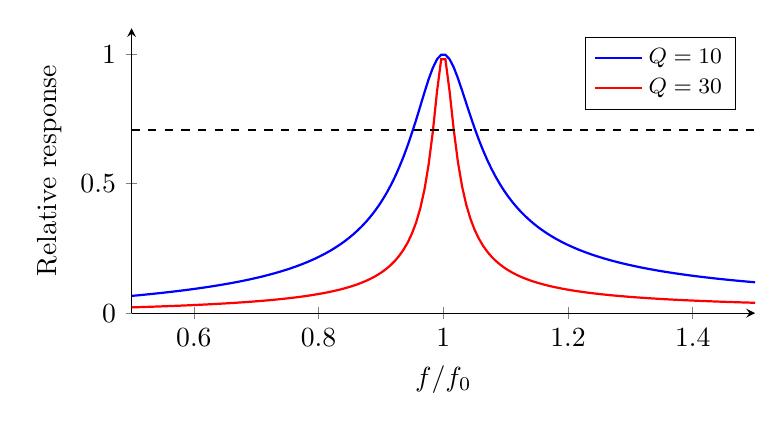
\begin{tikzpicture}
\begin{axis}[width=9.5cm,height=5.2cm,xlabel={$f/f_0$},ylabel={Relative response},
  xmin=0.5,xmax=1.5,ymin=0,ymax=1.1,domain=0.5:1.5,samples=150,
  axis lines=left,legend pos=north east, legend style={font=\footnotesize}]
\addplot[thick,blue] {1/sqrt(1+(10*(x-1/x))^2)};
\addlegendentry{$Q=10$}
\addplot[thick,red] {1/sqrt(1+(30*(x-1/x))^2)};
\addlegendentry{$Q=30$}
\draw[dashed] (axis cs:0.5,0.707) -- (axis cs:1.5,0.707) node[right,font=\footnotesize] {$-3$dB};
\end{axis}
\end{tikzpicture}
\end{center}

\begin{examplebox}[Bandwidth from Q]
A series-tuned circuit resonates at 7.1\,MHz with $L=2.5\,\mu$H,
$C=200\,\text{pF}$, and series resistance $R=3\,\Omega$. Find $Q$ and the
bandwidth.

\emph{Solution.}
\[
X_L = 2\pi f_0 L = 2\pi\times7.1\times10^6\times2.5\times10^{-6} \approx 111.5\,\Omega,
\]
\[
Q = \frac{X_L}{R} = \frac{111.5}{3} \approx 37.2, \qquad
B = \frac{f_0}{Q} = \frac{7.1\,\text{MHz}}{37.2} \approx 191\,\text{kHz}.
\]
\end{examplebox}

\section{Applications of Resonance in Radio}

\begin{itemize}
\item \textbf{Receiver front-end and IF selectivity}: tuned circuits
select the wanted signal and reject adjacent ones (Chapter~\ref{ch:receivers}).
\item \textbf{Transmitter output (tank) circuits}: convert an amplifying
device's output into a clean sinusoidal RF signal while suppressing
harmonics.
\item \textbf{Antenna tuning units}: use variable L and C to present a
resonant, well-matched impedance to a transmitter (Chapter~\ref{ch:transmission-lines}).
\item \textbf{Oscillators}: an LC tank sets the operating frequency of
many RF oscillator designs.
\item \textbf{Filters}: cascading multiple resonant sections builds the
band-pass, low-pass, and high-pass filters used throughout receivers and
transmitters (Chapter~\ref{ch:error-control} and Chapter~\ref{ch:receivers}).
\end{itemize}

\begin{quickreview}
\item Resonance occurs where $X_L = X_C$; $f_0 = 1/(2\pi\sqrt{LC})$ for
both series and parallel RLC circuits.
\item Series resonance: minimum impedance, maximum current (band-pass
behavior for current/output-across-R).
\item Parallel resonance (tank): maximum impedance, minimum line current
(band-reject as seen from outside; selects one frequency in a tank
application).
\item $Q = X/R$ at resonance; higher $Q$ means narrower bandwidth,
$B = f_0/Q$, and better selectivity but less tolerance and more loss
sensitivity.
\end{quickreview}

\begin{practiceproblems}
\item Find the resonant frequency of $L=4\,\mu$H, $C=68\,$pF.
\item A parallel tank has $R=10\,\text{k}\Omega$ (representing loss),
$L=1\,\mu$H, $C=400\,$pF. Find $f_0$ and $Q$.
\item A series-tuned circuit has $Q=50$ at $f_0=14.1\,$MHz. Find its
bandwidth.
\item Explain why a high-$Q$ circuit is more sensitive to small
component value changes than a low-$Q$ circuit.
\item A receiver needs to separate two signals 5\,kHz apart at
7.05\,MHz. Estimate the minimum $Q$ needed for a single resonant circuit
to provide meaningful separation (bandwidth on the order of the spacing).
\end{practiceproblems}

\chapter{Transformers}
\label{ch:transformers}

\section{Mutual Inductance and Transformer Action}

A \textbf{transformer} consists of two (or more) coils --- a
\textbf{primary} and a \textbf{secondary} --- wound so that they share a
common magnetic flux, usually by winding both around the same core. A
changing current in the primary produces a changing flux (Faraday's law,
Chapter~\ref{ch:fields}); that changing flux links the secondary winding
and induces an EMF there. No direct electrical (galvanic) connection is
required between primary and secondary --- energy is transferred
entirely through the shared magnetic field, which is why transformers
are the standard way to provide \textbf{galvanic isolation}, in addition
to voltage or impedance transformation.

\section{The Ideal Transformer Equations}

For an ideal transformer (no losses, all flux shared between windings),
the ratio of secondary to primary voltage equals the ratio of secondary
to primary turns, the \textbf{turns ratio}:
\[
\boxed{\frac{U_2}{U_1} = \frac{N_2}{N_1} = n}
\]
Conservation of power ($U_1 I_1 = U_2 I_2$ for an ideal, lossless
transformer) then requires current to transform in the \emph{inverse}
ratio:
\[
\frac{I_2}{I_1} = \frac{N_1}{N_2} = \frac{1}{n}.
\]
A \textbf{step-up} transformer ($N_2 > N_1$) raises voltage and lowers
current; a \textbf{step-down} transformer ($N_2 < N_1$) does the
opposite. Neither creates or destroys energy --- power in equals power
out for an ideal transformer.

\begin{examplebox}[Turns ratio]
A transformer has 1000 turns on the primary and 50 turns on the
secondary, with 230\,V RMS applied to the primary. Find the secondary
voltage, and the secondary current if the load draws 2\,A on the primary
side.

\emph{Solution.} Turns ratio $n = 50/1000 = 0.05$, so
$U_2 = 230 \times 0.05 = 11.5\,\text{V}$. Current transforms inversely:
$I_2 = I_1/n = 2/0.05 = 40\,\text{A}$.
\end{examplebox}

\section{Impedance Transformation}

Because a transformer changes the voltage-to-current ratio, it also
changes the \emph{impedance} seen looking into the primary for a given
load impedance $Z_2$ on the secondary:
\[
\boxed{Z_1 = n^2 Z_2}
\]
This impedance-transforming property is exploited constantly in RF
work: audio output transformers match a low-impedance speaker to a
higher-impedance amplifier stage, and RF transformers (including
\textbf{ferrite-core broadband transformers} wound with twisted or
bifilar wire) match a transmitter's output impedance to an antenna
system, or match one stage's impedance to the next, without the
narrowband limitation of an LC matching network.

\begin{examplebox}[Impedance matching]
Find the turns ratio needed to match a 50\,$\Omega$ source to an
800\,$\Omega$ load.

\emph{Solution.} Require $Z_1 = n^2 Z_2 \Rightarrow n = \sqrt{Z_1/Z_2} =
\sqrt{50/800} = \sqrt{1/16} = 0.25 = 1{:}4$. A turns ratio of 1:4
(primary:secondary) steps the 800\,$\Omega$ load down to an apparent
50\,$\Omega$ at the primary.
\end{examplebox}

\section{Real Transformers: Losses and Efficiency}

Real transformers depart from the ideal model in several ways:

\begin{itemize}
\item \textbf{Copper losses}: $I^2R$ heating in the winding resistance,
worse at high current (heavy secondary loading).
\item \textbf{Core losses}: hysteresis loss (energy needed to repeatedly
reverse the core material's magnetic domains) and eddy-current loss
(circulating currents induced within the core itself), both of which
increase with frequency --- one reason mains-frequency (50/60\,Hz) power
transformer cores cannot simply be reused, unmodified, at radio
frequencies.
\item \textbf{Leakage inductance}: flux produced by one winding that
does \emph{not} link the other winding, behaving as an unwanted series
inductance.
\item \textbf{Winding capacitance}: parasitic capacitance between turns
and between windings, which becomes significant at high frequency.
\end{itemize}

Efficiency is defined the same way as for any energy-conversion device:
\[
\eta = \frac{P_{\text{out}}}{P_{\text{in}}} \times 100\%.
\]
Well-designed power transformers commonly exceed 95\% efficiency at
rated load; efficiency generally drops at light load (core losses become
a larger fraction of a small output) and at heavy overload (copper
losses dominate and the core may begin to saturate).

\section{Autotransformers}

An \textbf{autotransformer} uses a single tapped winding rather than
electrically separate primary and secondary windings. It is smaller,
cheaper, and more efficient than an equivalent two-winding transformer
for a given power rating, but sacrifices galvanic isolation between
input and output --- an important safety distinction from a conventional
isolation transformer. Variable autotransformers (e.g., the classic
``Variac''-type device) are commonly used on the test bench to control AC
line voltage.

\section{RF Transformers and Baluns}

At radio frequencies, transformers are frequently wound on ferrite
toroid or binocular cores using twisted-pair or bifilar windings to
achieve tight coupling (high efficiency) over a wide bandwidth. A
particularly important RF application is the \textbf{balun}
(``balanced-to-unbalanced'' transformer), used to connect an unbalanced
coaxial feedline to a balanced antenna element such as a dipole
(Chapter~\ref{ch:antennas}) without upsetting the antenna's current
balance --- a common source of feedline radiation and RF-in-the-shack
problems if omitted or poorly chosen. A related device, the \textbf{unun}
(``unbalanced-to-unbalanced''), transforms impedance between two
unbalanced points, commonly used to match a random-wire or end-fed
antenna to a 50\,$\Omega$ coaxial feedline.

\begin{quickreview}
\item Transformer action relies on mutual inductance: a changing primary
current induces an EMF in a magnetically coupled secondary.
\item $U_2/U_1 = N_2/N_1 = n$; current transforms inversely, $I_2/I_1 =
1/n$; ideal power in equals power out.
\item Impedance transforms as $Z_1 = n^2 Z_2$ --- the basis of
transformer impedance matching.
\item Real transformers have copper loss, core loss (hysteresis and eddy
current), leakage inductance, and winding capacitance, all limiting
efficiency and bandwidth.
\item RF baluns and ununs are specialized transformers for connecting
balanced/unbalanced feedlines and antennas without disturbing current
balance.
\end{quickreview}

\begin{practiceproblems}
\item A transformer steps 120\,V down to 12\,V. If the primary turns
count is 600, find the secondary turns count.
\item Find the primary current if the secondary of the above transformer
delivers 3\,A to a load (assume ideal, lossless transformer).
\item Find the turns ratio needed to match a 50\,$\Omega$ transmitter
output to a 200\,$\Omega$ antenna feedpoint impedance.
\item A transformer delivers 90\,W output while consuming 100\,W input.
Find its efficiency, and name two loss mechanisms that could account for
the difference.
\item Explain why a balun is typically used where a coaxial feedline
connects to a dipole antenna, in terms of balanced vs.\ unbalanced
currents.
\end{practiceproblems}

\chapter{Power Sources and Batteries}
\label{ch:power-sources}

\section{Ideal and Real Sources}

An \textbf{ideal voltage source} maintains a fixed voltage regardless of
load current; an \textbf{ideal current source} maintains a fixed current
regardless of load voltage. Real sources (batteries, power supplies,
generators) approximate the ideal voltage source but have a small
\textbf{internal resistance} $R_{\text{int}}$ in series, which causes the
terminal voltage to sag under load:
\[
\boxed{U_{\text{terminal}} = \text{EMF} - I R_{\text{int}}}
\]
This single equation explains why a weak or discharged battery's voltage
recovers somewhat when a load is removed (the $IR_{\text{int}}$ drop
disappears) and why a heavily loaded supply's voltage is lower than its
open-circuit (no-load) rating.

\begin{examplebox}[Voltage sag under load]
A 12\,V battery with internal resistance 0.2\,$\Omega$ supplies 8\,A to a
transceiver. Find the terminal voltage.

\emph{Solution.}
\[
U_{\text{terminal}} = 12 - (8 \times 0.2) = 12 - 1.6 = 10.4\,\text{V}.
\]
This sag is one reason mobile/portable radio equipment often specifies a
minimum operating voltage below the nominal 12\,V or 13.8\,V rating.
\end{examplebox}

\section{Maximum Power Transfer}

For a source with fixed internal resistance $R_{\text{int}}$ driving a
variable load $R_L$, the power delivered \emph{to the load} is maximized
when $R_L = R_{\text{int}}$ (the \textbf{maximum power transfer
theorem}) --- at that point exactly half the source's total generated
power is delivered to the load and half is dissipated internally, so
this condition maximizes load power but not overall efficiency. This
principle underlies impedance-matching practice throughout RF systems
(Chapter~\ref{ch:transmission-lines}): matching source and load
impedance maximizes power transfer, though in power-supply and battery
contexts, efficiency (minimizing $R_{\text{int}}$ relative to the load)
is usually the more relevant goal instead.

\section{Cells and Batteries}

A single electrochemical \textbf{cell} converts stored chemical energy
into electrical energy; a \textbf{battery} is one or more cells combined
(in series for higher voltage, in parallel for higher capacity, or both).

\begin{center}
\renewcommand{\arraystretch}{1.2}
\begin{tabularx}{\linewidth}{@{}l l l l Y@{}}
\toprule
Chemistry & Cell V & Rechg.? & Energy density & Notes \\
\midrule
Alkaline (Zn-MnO$_2$) & 1.5\,V & No & Low & Cheap, common, poor at high current \\
NiMH & 1.2\,V & Yes & Moderate & Low self-discharge (LSD) types common \\
Lead-acid & 2.0\,V/cell & Yes & Low--mod. & High current capable; heavy \\
Li-ion & 3.6--3.7\,V & Yes & High & Requires protection circuitry \\
LiFePO$_4$ & 3.2\,V & Yes & High & Safer chemistry, flatter discharge curve \\
\bottomrule
\end{tabularx}
\end{center}

\subsection{Series and Parallel Battery Combinations}

\begin{keyidea}
\textbf{Cells in series} add voltage; capacity (in amp-hours) stays the
same as a single cell. \textbf{Cells in parallel} add capacity; voltage
stays the same as a single cell. A common 12\,V lead-acid battery is
internally six 2\,V cells in series.
\end{keyidea}

\begin{safetynote}[Mixing cells]
Never combine cells of different chemistry, capacity, or state of charge
in the same series or parallel string. Mismatched cells can be forced
into reverse charge, over-discharge, or unequal current sharing, any of
which can cause overheating, venting, or fire --- especially with
lithium-based chemistries, which additionally require dedicated
protection/balancing circuitry in multi-cell packs.
\end{safetynote}

\section{Amp-Hour Capacity and Runtime}

Battery capacity is rated in \textbf{amp-hours (Ah)} or milliamp-hours
(mAh) --- a direct application of $Q = It$ from
Chapter~\ref{ch:electricity}, expressed with $t$ in hours instead of
seconds. Approximate runtime for a given load current is
\[
t \approx \frac{\text{Capacity (Ah)}}{I_{\text{load}} (\text{A})}
\]
(approximate because usable capacity typically falls at high discharge
current, a behavior described empirically by \textbf{Peukert's law} for
lead-acid batteries, and because most chemistries should not be
discharged to 0\% without damage or reduced cycle life).

\begin{examplebox}[Estimating runtime]
A handheld transceiver draws 300\,mA average on receive and is powered
by a 2000\,mAh battery. Estimate the receive-only runtime.

\emph{Solution.}
\[
t \approx \frac{2000\,\text{mAh}}{300\,\text{mA}} \approx 6.7\,\text{hours}.
\]
Real-world runtime will be shorter due to periods of transmit current
(much higher than receive current) and capacity derating at higher
discharge rates.
\end{examplebox}

Energy capacity in watt-hours (useful for comparing different battery
voltages on an equal footing) is
\[
W_h = \text{Ah} \times U_{\text{nominal}}.
\]

\section{Charging Considerations}

Different chemistries require different charge algorithms (constant
current then constant voltage for Li-ion; different profiles for NiMH
and lead-acid), and using the wrong charger or charge rate can
permanently damage capacity, or in the case of lithium chemistries,
create a serious fire hazard. \textbf{C-rate} notation describes charge
or discharge current relative to capacity: a ``1C'' rate for a 2\,Ah
battery is 2\,A; a ``0.5C'' rate is 1\,A.

\section{DC Power Supplies}

A mains-powered DC \textbf{power supply} typically consists of a
transformer (Chapter~\ref{ch:transformers}) to change AC mains voltage
to a convenient level, a rectifier (diodes, Chapter~\ref{ch:semiconductors})
to convert AC to pulsating DC, a filter capacitor to smooth the
pulsations into a nearly steady DC voltage, and a voltage regulator to
hold the output constant despite input ripple and load changes. A
\textbf{linear regulator} dissipates the voltage difference between
input and output as heat (simple, low-noise, but inefficient at large
voltage drops); a \textbf{switching regulator} rapidly switches a
storage inductor or capacitor to convert voltage with much higher
efficiency, at the cost of potential RF noise/interference that must be
filtered --- a genuine concern for a radio amateur choosing a supply to
sit next to a sensitive receiver.

\begin{quickreview}
\item Real sources sag under load: $U_{\text{terminal}} = \text{EMF} -
IR_{\text{int}}$.
\item Maximum power transfer occurs when load resistance equals source
internal resistance.
\item Series cells add voltage; parallel cells add capacity; never mix
chemistries, capacities, or states of charge in a pack.
\item Capacity (Ah) combined with load current gives approximate runtime,
$t \approx \text{Ah}/I$; watt-hours allow comparison across voltages.
\item Linear regulators are simple and quiet but lossy; switching
regulators are efficient but can generate RF interference.
\end{quickreview}

\begin{practiceproblems}
\item A power supply has an open-circuit voltage of 13.8\,V and internal
resistance 0.05\,$\Omega$. Find the terminal voltage at a 20\,A load.
\item Four 1.2\,V, 2000\,mAh NiMH cells are connected in series. Find the
resulting pack voltage and capacity.
\item Estimate the runtime of a 7\,Ah battery supplying a constant 1.4\,A
load.
\item Explain, using $Q=It$, why amp-hours (not just amps) are the
correct way to compare battery ``size.''
\item A radio amateur reports RF hash/noise across several bands after
switching from a linear to a switching power supply. Explain a likely
cause and one practical mitigation.
\end{practiceproblems}


\part{Active Devices and RF Systems}
\chapter{Semiconductors, Diodes, and Transistors}
\label{ch:semiconductors}

\section{Doping and the p-n Junction}

Pure (\textbf{intrinsic}) silicon is a poor conductor. Deliberately
introducing trace impurities (\textbf{doping}) transforms its
conductivity in a controllable way: adding an element with one more
valence electron than silicon (phosphorus, arsenic) creates
\textbf{n-type} material with an excess of free electrons; adding an
element with one fewer valence electron (boron) creates \textbf{p-type}
material with an excess of ``holes'' (missing-electron sites that behave
as mobile positive charge carriers).

Where p-type and n-type materials meet, a \textbf{p-n junction} forms.
Electrons and holes diffuse across the junction and recombine near the
boundary, leaving a thin \textbf{depletion region} depleted of free
carriers and building a small internal electric field that opposes
further diffusion. This junction is the foundation of essentially every
semiconductor device in electronics.

\section{The Diode}

A \textbf{diode} is a single p-n junction packaged with two terminals,
the \textbf{anode} (p-side) and \textbf{cathode} (n-side). It conducts
current easily in one direction (\textbf{forward bias}, anode positive
relative to cathode) once the applied voltage exceeds a threshold ---
about 0.6--0.7\,V for silicon, 0.2--0.3\,V for germanium, and roughly
1.8--3.3\,V (varying by color/wavelength) for light-emitting diodes ---
and blocks current almost completely in the opposite direction
(\textbf{reverse bias}), up to a maximum reverse voltage rating beyond
which it breaks down.

\begin{center}
\begin{circuitikz}
\draw (0,0) to[battery1,l=$U$] (0,2) to[D,l=diode] (3,2) to[R,l=$R$] (3,0) -- (0,0);
\end{circuitikz}
\end{center}

\subsection{Diode Types and RF/Amateur Applications}

\begin{itemize}
\item \textbf{Rectifier diodes}: convert AC to pulsating DC in power
supplies (Chapter~\ref{ch:power-sources}).
\item \textbf{Zener diodes}: designed to operate safely in reverse
breakdown at a well-defined voltage, used as simple voltage references
or shunt regulators.
\item \textbf{Varactor (varicap) diodes}: reverse-biased junction
capacitance varies with applied voltage, used for electronic tuning in
VFOs and PLL synthesizers.
\item \textbf{Schottky diodes}: metal-semiconductor junction with a
lower forward voltage drop and much faster switching than a standard
silicon junction diode, widely used in RF detectors and mixers.
\item \textbf{PIN diodes}: behave as a variable resistor at RF when
forward-biased with varying DC current, used as RF switches and
attenuators (e.g., for T/R switching).
\item \textbf{Light-emitting diodes (LEDs)}: emit light when forward
biased, used for indicators and, in laser diode form, for optical
communication experiments.
\end{itemize}

\section{Bipolar Junction Transistors (BJTs)}

A \textbf{bipolar junction transistor} adds a second junction, forming
either an \textbf{NPN} or \textbf{PNP} sandwich of doped regions ---
\textbf{emitter}, \textbf{base}, and \textbf{collector}. A BJT is a
\textbf{current-controlled current source}: a small current flowing into
the base controls a much larger current flowing from collector to
emitter (NPN), with the ratio between them called \textbf{current gain},
$\beta$ (or $h_{FE}$):
\[
\boxed{I_C = \beta I_B}, \qquad I_E = I_B + I_C.
\]
Typical small-signal transistors have $\beta$ in the range of roughly
50--300. This current-controlled amplification is the basic mechanism
behind BJT amplifier and switching circuits.

\begin{center}
\begin{circuitikz}
\draw (0,0) node[npn](Q1){}
  (Q1.base) node[left]{B}
  (Q1.collector) node[above]{C}
  (Q1.emitter) node[below]{E};
\end{circuitikz}
\end{center}

\subsection{Common Amplifier Configurations}

\begin{itemize}
\item \textbf{Common-emitter}: input at base, output at collector,
emitter grounded (often through a small resistor). High voltage and
current gain, inverts the signal ($180\degree$ phase shift), moderate
input/output impedance --- the most common general-purpose amplifier
configuration.
\item \textbf{Common-base}: input at emitter, output at collector, base
grounded (at AC). Low input impedance, high output impedance, no phase
inversion, good high-frequency performance --- often used in RF
amplifier and mixer stages.
\item \textbf{Common-collector} (\textbf{emitter follower}): input at
base, output at emitter, collector grounded (at AC). Voltage gain near
unity, but high current gain and impedance transformation (high input
impedance, low output impedance) --- widely used as a buffer stage.
\end{itemize}

\section{Field-Effect Transistors (FETs)}

A \textbf{field-effect transistor} is a \textbf{voltage-controlled
current source}: a voltage applied to the \textbf{gate} controls current
flowing between \textbf{drain} and \textbf{source}, with (ideally) no
gate current at all --- giving FETs an extremely high input impedance,
in contrast to the current-driven BJT.

\begin{itemize}
\item \textbf{JFET} (junction FET): gate forms a reverse-biased junction
with the channel; normally ``on,'' with gate voltage used to pinch the
channel off.
\item \textbf{MOSFET} (metal-oxide-semiconductor FET): gate is insulated
from the channel by a thin oxide layer, giving even higher input
impedance than a JFET; available in \textbf{enhancement mode} (normally
off, turned on by gate voltage --- the dominant type in digital logic
and switching power supplies) and \textbf{depletion mode} (normally on).
\end{itemize}

MOSFETs, particularly power MOSFETs, are widely used in RF power
amplifiers and switching applications for amateur equipment because of
their high input impedance, ease of biasing, and good high-frequency
switching behavior.

\begin{safetynote}[Static sensitivity]
MOSFET gates are separated from the channel by an extremely thin
insulating layer that can be punctured by static discharge well below
the voltage a person can even feel. Handle MOSFETs and other
static-sensitive devices using proper ESD precautions (grounded
workstation, anti-static packaging) until they are soldered into a
circuit.
\end{safetynote}

\section{The Transistor as a Switch}

Beyond linear amplification, both BJTs and FETs are used as electronic
\textbf{switches}: driven fully ``on'' (\textbf{saturation} for a BJT,
low on-resistance for a MOSFET) or fully ``off'' (\textbf{cutoff}), a
transistor can control power to a load (a relay, a keying line, a
transmitter's PTT circuit) with a small control signal, forming the
building block of digital logic gates and switch-mode power circuits.

\section{Integrated Circuits}

An \textbf{integrated circuit (IC)} fabricates many transistors (from a
handful to billions), along with diodes, resistors, and sometimes small
capacitors, on a single piece of semiconductor material. This allows
complex functions --- operational amplifiers (Chapter~\ref{ch:opamps}),
digital logic, microcontrollers, RF mixers, phase-locked loop
synthesizers, and entire radio transceivers --- to be built far more
compactly, reliably, and cheaply than from discrete components, and
underlies essentially all modern amateur radio equipment design.

\begin{quickreview}
\item Doping creates n-type (excess electrons) and p-type (excess holes)
semiconductor material; a p-n junction is the basic building block.
\item Diodes conduct in one direction above a forward-voltage threshold
and block in reverse, up to a breakdown limit; many specialized diode
types (Zener, varactor, Schottky, PIN, LED) exploit particular junction
behaviors.
\item BJTs are current-controlled ($I_C = \beta I_B$); FETs are
voltage-controlled with very high input impedance.
\item Common-emitter, common-base, and common-collector configurations
trade off gain, impedance, and phase behavior differently.
\item Transistors are used both as linear amplifiers and as switches;
ICs integrate many transistors and other components on one chip.
\end{quickreview}

\begin{practiceproblems}
\item A BJT has $\beta = 100$ and $I_B = 50\,\mu\text{A}$. Find $I_C$ and
$I_E$.
\item Explain why a MOSFET's gate current is essentially zero in normal
operation, in terms of its construction.
\item Name one diode type suited to (a) voltage regulation, (b)
electronic tuning, (c) fast RF detection, and briefly justify each
choice.
\item Explain why an emitter-follower stage, despite having voltage gain
near 1, is still a useful amplifier configuration.
\item A technician reports a MOSFET failed immediately upon handling
before installation, with no circuit fault found. Suggest a likely
cause and a preventive measure.
\end{practiceproblems}

\chapter{Operational Amplifiers}
\label{ch:opamps}

\section{The Ideal Op-Amp}

An \textbf{operational amplifier (op-amp)} is a high-gain differential
voltage amplifier IC, so widely used as a building block that it is
treated as a component in its own right rather than analyzed
transistor-by-transistor. It has two inputs --- the \textbf{non-inverting
input} ($+$) and the \textbf{inverting input} ($-$) --- and one output,
and amplifies the \emph{difference} between its two inputs by an
enormous open-loop gain (typically $10^5$ or more).

\bookfig[0.55]{opamp_internal.png}{A simplified internal structure of an
operational amplifier: differential input stage, gain stage, and output
stage.}

\begin{keyidea}[The two golden rules of ideal op-amp analysis]
When an op-amp is used with \textbf{negative feedback} (a path from the
output back to the inverting input), two simplifying assumptions make
hand analysis of nearly any op-amp circuit tractable:
\begin{enumerate}
\item \textbf{No current flows into either input} (the inputs have
essentially infinite impedance).
\item \textbf{The output adjusts itself so that the voltage difference
between the two inputs is zero} (``virtual short''), provided the
feedback loop is intact and the output is not saturated.
\end{enumerate}
\end{keyidea}

\section{The Inverting Amplifier}

\begin{center}
\begin{circuitikz}
\draw (0,2) to[R,l=$R_1$,-*] (2,2) node[op amp,anchor=-,scale=1.3](opamp){};
\draw (opamp.+) to[short] ++(-0.6,0) node[ground]{};
\draw (opamp.out) -- ++(0.8,0) node[right](out){$U_{\text{out}}$};
\draw (2,2) to[R,l=$R_f$] (2,3.2) -| (out.center) node[near end,above]{};
\draw (0,2) node[left]{$U_{\text{in}}$};
\end{circuitikz}
\end{center}

With the input applied through $R_1$ to the inverting input and feedback
resistor $R_f$ from output back to that same node, the ``virtual short''
rule forces the inverting input to sit at 0\,V (since the non-inverting
input is grounded), so the same current flows through $R_1$ and $R_f$.
The result is the widely used \textbf{inverting amplifier} gain formula:
\[
\boxed{A_v = \frac{U_{\text{out}}}{U_{\text{in}}} = -\frac{R_f}{R_1}}
\]
The negative sign indicates $180\degree$ phase inversion. Gain is set
purely by the ratio of two resistors, independent (to a good
approximation) of the op-amp's own large and imprecisely specified
open-loop gain --- the central practical benefit of negative feedback.

\begin{examplebox}[Inverting amplifier gain]
$R_1 = 10\,\text{k}\Omega$, $R_f = 100\,\text{k}\Omega$. Find the gain,
and the output voltage for a $-0.2\,\text{V}$ input.

\emph{Solution.}
\[
A_v = -\frac{R_f}{R_1} = -\frac{100}{10} = -10, \qquad
U_{\text{out}} = A_v \times U_{\text{in}} = -10 \times (-0.2) = 2\,\text{V}.
\]
\end{examplebox}

\section{The Non-Inverting Amplifier}

Applying the input directly to the non-inverting input, with a feedback
network ($R_f$ and $R_1$ to ground) setting the inverting input to a
fraction of the output, gives:
\[
\boxed{A_v = 1 + \frac{R_f}{R_1}}
\]
Gain is always $\geq 1$ and the output is \emph{in phase} with the
input (no inversion). Setting $R_f = 0$ (or removing it and connecting
output directly to the inverting input) gives $A_v = 1$: the
\textbf{voltage follower} (buffer), used purely for its extremely high
input impedance and low output impedance, without adding voltage gain.

\section{Other Common Op-Amp Circuits}

\begin{itemize}
\item \textbf{Summing amplifier}: multiple input resistors into the
inverting node combine several input voltages with individually
weighted gains, output being the (inverted, scaled) sum --- used in
audio mixing and analog computation.
\item \textbf{Differential amplifier}: amplifies the difference between
two input signals while rejecting any voltage common to both
(\textbf{common-mode rejection}) --- useful for extracting a small
signal riding on a larger common noise voltage.
\item \textbf{Integrator / differentiator}: replacing a resistor with a
capacitor in the feedback or input path produces a circuit whose output
is proportional to the time-integral or time-derivative of the input,
used in filter, waveform-shaping, and control applications.
\item \textbf{Active filters}: op-amps combined with RC networks
implement precise low-pass, high-pass, and band-pass filters (audio CW
and SSB filtering in receivers is a direct amateur radio application)
without the bulky inductors that a purely passive filter would need at
audio frequencies.
\item \textbf{Comparator}: an op-amp used without negative feedback (or
with positive feedback for hysteresis) simply drives its output to one
supply rail or the other depending on which input is higher --- used for
squelch circuits, threshold detection, and simple ADC building blocks.
\end{itemize}

\section{Real Op-Amp Limitations}

\begin{itemize}
\item \textbf{Finite open-loop gain and bandwidth}: gain is not
literally infinite, and it falls off with frequency (the
\textbf{gain-bandwidth product}, GBW, is a key datasheet specification
--- a 1\,MHz GBW device configured for a gain of 100 will only be
usable up to roughly 10\,kHz).
\item \textbf{Slew rate}: a maximum rate of change the output can
follow, in V/$\mu$s --- limits large-signal high-frequency performance
even within the small-signal bandwidth.
\item \textbf{Input offset voltage and bias current}: small
imperfections that cause a nonzero output even with both inputs
grounded, of particular concern in high-precision or high-gain DC
applications.
\item \textbf{Output swing and current limits}: the output cannot
exceed the supply rails (often not quite reaching them either, unless
the device is specifically a ``rail-to-rail'' design) and can only
supply a limited current before distorting or current-limiting.
\end{itemize}

Standard general-purpose op-amps (with gain-bandwidth products in the
single-digit MHz) are used extensively in amateur radio audio stages ---
receiver audio filtering, AGC (automatic gain control) generation, CW
sidetone oscillators, and microphone amplifiers --- but are generally
unsuitable as direct RF amplifiers at HF and above without specialized
high-speed devices, for which dedicated RF amplifier ICs or discrete
transistor stages (Chapter~\ref{ch:semiconductors}) are typically used
instead.

\begin{quickreview}
\item Ideal op-amp analysis: no current into either input; feedback
forces the two inputs to the same voltage (virtual short).
\item Inverting amplifier: $A_v = -R_f/R_1$ (inverted, gain set by
resistor ratio).
\item Non-inverting amplifier: $A_v = 1+R_f/R_1$ (in phase, gain
$\geq1$); $R_f=0$ gives a unity-gain buffer.
\item Summing, differential, integrator/differentiator, active filter,
and comparator circuits all build on the same two golden rules.
\item Real op-amps have finite gain-bandwidth product, slew rate, offset
errors, and output swing/current limits.
\end{quickreview}

\begin{practiceproblems}
\item Design an inverting amplifier with gain $-20$ using
$R_1=1\,\text{k}\Omega$; find the required $R_f$.
\item A non-inverting amplifier uses $R_1=2\,\text{k}\Omega$,
$R_f=18\,\text{k}\Omega$. Find the gain and the output for a 0.1\,V
input.
\item An op-amp has a gain-bandwidth product of 3\,MHz. Estimate the
maximum usable frequency at a closed-loop gain of 50.
\item Explain, using the golden rules, why the inverting input of an
inverting amplifier is called a ``virtual ground'' even though it is not
physically connected to ground.
\item Explain why a voltage-follower (buffer) stage is useful even
though its voltage gain is only 1.
\end{practiceproblems}

\chapter{Decibels, Gain, and Loss}
\label{ch:decibels}

\section{Why Use a Logarithmic Unit?}

A radio signal chain often includes many stages, each multiplying power
by some factor: an antenna's gain, a length of feedline's loss, a
preamplifier's gain, a filter's loss, a receiver's sensitivity. Multiplying
many such ratios together by hand is tedious and error-prone; expressed
logarithmically (Chapter~\ref{ch:units}), those same ratios simply
\emph{add}. This is the entire motivation for the \textbf{decibel (dB)},
one-tenth of a \textbf{bel} (named for Alexander Graham Bell), and the
single most-used unit in RF system-level work.

\section{Defining the Decibel}

For \textbf{power} ratios,
\[
\boxed{dB = 10\log_{10}\!\left(\frac{P_2}{P_1}\right)}
\]
For \textbf{voltage} (or current) ratios measured across the \emph{same}
impedance, since power is proportional to voltage squared
($P = U^2/R$), the factor of 2 from squaring moves in front of the log:
\[
\boxed{dB = 20\log_{10}\!\left(\frac{U_2}{U_1}\right)}
\]

\begin{keyidea}[Values worth memorizing]
\begin{center}
\begin{tabular}{@{}rll@{}}
\toprule
Ratio & Power (dB) & Voltage (dB) \\
\midrule
$\times 1$ & 0\,dB & 0\,dB \\
$\times 2$ & 3\,dB & 6\,dB \\
$\times 4$ & 6\,dB & 12\,dB \\
$\times 10$ & 10\,dB & 20\,dB \\
$\times 100$ & 20\,dB & 40\,dB \\
$\div 2$ & $-3$\,dB & $-6$\,dB \\
$\div 10$ & $-10$\,dB & $-20$\,dB \\
\bottomrule
\end{tabular}
\end{center}
``3\,dB'' meaning a doubling (or, negative, a halving) \emph{of power}
is one of the most exam-relevant and practically useful facts in this
entire book --- it is the basis for the $-3\,\text{dB}$ (half-power)
bandwidth points used to define filter and resonance bandwidth
(Chapter~\ref{ch:rlc-resonance}).
\end{keyidea}

\begin{examplebox}[Cascaded gains and losses]
A signal passes through a preamplifier (+12\,dB), a length of coaxial
cable ($-2\,\text{dB}$), and a filter ($-1.5\,\text{dB}$). Find the net
gain or loss.

\emph{Solution.} Because decibels represent logarithms of ratios, they
simply add along a cascade:
\[
12 + (-2) + (-1.5) = 8.5\,\text{dB (net gain)}.
\]
Multiplying the equivalent linear power ratios directly
($10^{1.2}\times10^{-0.2}\times10^{-0.15} \approx 15.85\times0.631\times0.708
\approx 7.08$, i.e.\ $10\log_{10}(7.08)\approx8.5\,\text{dB}$) confirms
the same result --- but the addition is far faster.
\end{examplebox}

\section{Converting Between dB and Linear Ratios}

To go the other direction, from a dB value back to a plain ratio:
\[
\frac{P_2}{P_1} = 10^{(dB/10)}, \qquad \frac{U_2}{U_1} = 10^{(dB/20)}.
\]

\begin{examplebox}[dB to linear]
An amplifier is specified with 20\,dB of gain. Find the power ratio and
the voltage ratio it represents.

\emph{Solution.}
\[
\frac{P_2}{P_1} = 10^{20/10} = 10^2 = 100, \qquad
\frac{U_2}{U_1} = 10^{20/20} = 10^1 = 10.
\]
\end{examplebox}

\section{Absolute Levels: dBm, dBW, and dBi}

The decibel itself is always a \emph{ratio} (dimensionless); appending a
reference to the unit turns it into an absolute level:

\begin{itemize}
\item \textbf{dBm}: power relative to 1\,milliwatt.
\[
P(\text{dBm}) = 10\log_{10}\!\left(\frac{P(\text{mW})}{1\,\text{mW}}\right).
\]
0\,dBm = 1\,mW; 30\,dBm = 1\,W; 60\,dBm = 1\,kW. dBm is the standard unit
for receiver sensitivity specifications, signal levels at a mixer or
amplifier input, and RF test equipment readouts.
\item \textbf{dBW}: power relative to 1\,watt; $0\,\text{dBW} =
30\,\text{dBm}$, used for higher-power figures such as transmitter
output or effective radiated power.
\item \textbf{dBi}: antenna gain relative to a theoretical
\textbf{isotropic radiator} (a point source radiating equally in all
directions) --- the standard way antenna gain is specified
(Chapter~\ref{ch:antennas}).
\item \textbf{dBd}: antenna gain relative to a reference half-wave
dipole; $\text{dBi} = \text{dBd} + 2.15$, since a dipole itself has
2.15\,dBi of gain over an isotropic radiator.
\end{itemize}

\begin{examplebox}[dBm arithmetic]
A transmitter delivers 100\,W to a feedline with 3\,dB of loss, feeding
an antenna with 6\,dBi of gain. Find the effective radiated power (ERP,
referenced to a dipole, or EIRP referenced to isotropic).

\emph{Solution.} Convert 100\,W to dBW: $10\log_{10}(100) =
20\,\text{dBW}$. Apply cascade addition:
\[
20\,\text{dBW} - 3\,\text{dB} + 6\,\text{dBi} = 23\,\text{dBW (EIRP)}.
\]
Converting back: $10^{23/10} \approx 200\,\text{W EIRP}$ --- twice the
transmitter's output power, because the antenna gain (6\,dB $\approx
\times4$) outweighs the feedline loss (3\,dB $\approx \div2$).
\end{examplebox}

\section{Signal-to-Noise Ratio}

\textbf{Signal-to-noise ratio (SNR)}, expressed in dB, compares wanted
signal power to unwanted noise power at the same point in a system:
\[
\text{SNR (dB)} = 10\log_{10}\!\left(\frac{P_{\text{signal}}}{P_{\text{noise}}}\right).
\]
SNR is the single most important figure of merit for whether a
communication link will be intelligible; it reappears throughout
Chapters~\ref{ch:receivers} (receiver noise figure) and
\ref{ch:propagation} (link budgets), and is a core concept behind
digital mode weak-signal performance (Chapter~\ref{ch:digital-modes}).

\begin{quickreview}
\item Power ratio in dB: $10\log_{10}(P_2/P_1)$; voltage ratio in dB:
$20\log_{10}(U_2/U_1)$.
\item Cascaded gains/losses simply add in dB (versus multiplying as
linear ratios).
\item Memorize: $+3\,\text{dB} \approx \times2$ power,
$+10\,\text{dB} = \times10$ power, $+6\,\text{dB} \approx \times2$
voltage/current, $+20\,\text{dB} = \times10$ voltage/current.
\item dBm (ref.\ 1\,mW), dBW (ref.\ 1\,W), dBi (ref.\ isotropic
antenna), dBd (ref.\ dipole, $= \text{dBi} - 2.15$) are absolute levels
built on the relative dB unit.
\item SNR in dB compares signal to noise power and is the key
determinant of link intelligibility.
\end{quickreview}

\begin{practiceproblems}
\item Convert a power ratio of 500 into dB.
\item Convert $-6\,\text{dB}$ into a linear voltage ratio.
\item A receiver preamplifier has 15\,dB gain; a following filter has
2.5\,dB loss. Find the net dB and the equivalent linear power ratio.
\item Convert 5\,W to dBm.
\item An antenna is rated at 9\,dBd. Express this gain in dBi.
\end{practiceproblems}

\chapter{Receiver Architectures}
\label{ch:receivers}

A radio receiver's job is to select one wanted signal from among the
enormous number of other signals and noise present at its antenna,
convert it to a usable form, and produce audio (or digital data) with
adequate signal-to-noise ratio and freedom from interference. This
chapter surveys the major receiver architectures used from the earliest
days of radio to the present.

\section{Key Receiver Performance Concepts}

\begin{itemize}
\item \textbf{Sensitivity}: the weakest signal a receiver can usefully
detect, limited ultimately by internally generated noise (thermal noise
in resistive elements and semiconductor devices), quantified by the
receiver's \textbf{noise figure} (how much noisier the receiver is than
an ideal noiseless one, in dB).
\item \textbf{Selectivity}: the receiver's ability to reject signals on
frequencies close to the wanted one, set largely by its filter
bandwidth and shape (Chapter~\ref{ch:rlc-resonance}).
\item \textbf{Dynamic range}: the span, in dB, between the weakest
signal the receiver can detect and the strongest signal it can handle
without unacceptable distortion (\textbf{overload} or
\textbf{intermodulation distortion}, where two or more strong nearby
signals mix together inside a nonlinear stage to create spurious
``phantom'' signals).
\item \textbf{Image rejection}: the ability to reject an unwanted
frequency that a mixing stage would otherwise convert to the same output
frequency as the wanted signal (Section~\ref{sec:superhet} below).
\end{itemize}

\section{Tuned Radio Frequency (TRF) Receivers}

\bookfig[0.55]{receptor_trf.png}{Block diagram of a tuned radio
frequency (TRF) receiver.}

The earliest practical receiver architecture amplifies the incoming
signal directly at its original (radio) frequency through one or more
stages of RF amplification, each individually tuned to the wanted
frequency, before demodulating it. TRF receivers are conceptually
simple but have a fundamental weakness: keeping several separate tuned
stages aligned to exactly the same frequency as the operator tunes
across the band is mechanically difficult, and selectivity (which
depends on $Q$, Chapter~\ref{ch:rlc-resonance}) is hard to make
uniformly good across a wide tuning range, since a fixed-$Q$ circuit's
absolute bandwidth changes with frequency.

\section{Direct Conversion Receivers}

\bookfig[0.55]{receptor_convdirecta.png}{Block diagram of a direct
conversion receiver.}

A \textbf{direct conversion} receiver mixes the incoming RF signal
directly with a local oscillator (LO) set to (nearly) the same
frequency as the wanted signal, producing an output directly at audio
frequency (the mixing process is developed fully in
Chapter~\ref{ch:modulation}). This is simpler than a superheterodyne
design (fewer stages, no IF filter needed) and is popular in simple and
homebrew equipment, but suffers from being susceptible to
\textbf{audio-frequency image response} (signals above and below the LO
frequency both fold into the same audio output, requiring phasing
techniques to separate sidebands) and generally offers less overall
selectivity than a well-designed superheterodyne.

\section{The Superheterodyne Receiver}
\label{sec:superhet}

\bookfig[0.6]{receptor_superhet.png}{Block diagram of a superheterodyne
receiver.}

The \textbf{superheterodyne} (``superhet''), developed by Edwin
Armstrong and still the dominant architecture (now often implemented
digitally rather than with discrete analog stages), solves the TRF
alignment problem by converting every incoming signal to a fixed
\textbf{intermediate frequency (IF)}, regardless of the tuned frequency,
using a mixer and a tunable local oscillator:
\[
\boxed{f_{\text{IF}} = |f_{\text{signal}} - f_{\text{LO}}|}
\]
Because the IF is fixed, the bulk of the receiver's gain and
selectivity can be built once, at a single frequency, using
well-optimized fixed-tuned filters (often crystal or ceramic filters)
--- giving consistently good, easily reproducible selectivity across the
entire tuning range, the key advantage over a TRF design.

\subsection{The Image Frequency Problem}

Because the mixer output depends only on the \emph{difference} between
signal and LO frequency, \emph{two} input frequencies produce the same
IF output: the wanted signal at $f_{\text{LO}} + f_{\text{IF}}$ (or
$f_{\text{LO}} - f_{\text{IF}}$) and an unwanted \textbf{image
frequency} on the opposite side of the LO, offset by exactly
$2f_{\text{IF}}$ from the wanted signal:
\[
f_{\text{image}} = f_{\text{signal}} \pm 2f_{\text{IF}}.
\]

\begin{examplebox}[Finding an image frequency]
A receiver tuned to 14.200\,MHz uses a 9.000\,MHz IF and high-side
injection ($f_{\text{LO}} = f_{\text{signal}} + f_{\text{IF}} =
23.200\,\text{MHz}$). Find the image frequency.

\emph{Solution.}
\[
f_{\text{image}} = f_{\text{LO}} + f_{\text{IF}} = 23.200 + 9.000 = 32.200\,\text{MHz}.
\]
(Equivalently, $f_{\text{signal}} + 2f_{\text{IF}} = 14.200 + 18.000 =
32.200\,\text{MHz}$.) A signal at 32.200\,MHz, if not rejected before the
mixer, would appear at the same 9.000\,MHz IF as the wanted 14.200\,MHz
signal.
\end{examplebox}

\begin{keyidea}[Fighting the image]
Image rejection is provided by front-end filtering \emph{before} the
mixer. A \emph{higher} IF pushes the image frequency further away from
the wanted signal (easier to filter with a simple front-end filter), but
makes it harder to build a narrow, high-selectivity IF filter at that
higher frequency (Chapter~\ref{ch:rlc-resonance}: absolute bandwidth for
a given $Q$ grows with frequency). This trade-off is why many
modern receivers use a high first IF for good image rejection, followed
by conversion to a lower second IF for good adjacent-channel
selectivity --- a \textbf{dual (or multiple) conversion} superheterodyne.
\end{keyidea}

\section{The Superregenerative Receiver}

\bookfig[0.5]{receptor_superreg.png}{A simplified superregenerative
detector.}

A \textbf{superregenerative} receiver deliberately drives a single RF
amplifier stage into and out of oscillation at a rapid (typically
ultrasonic) rate, exploiting the huge effective gain available right at
the threshold of oscillation to achieve remarkable sensitivity from a
very small number of components. It trades selectivity and
linearity for extreme simplicity and low cost, and remains common in
inexpensive, short-range devices (some remote controls and simple
telemetry receivers) despite being essentially obsolete for
general-purpose amateur communication receivers.

\section{Software-Defined Radio (SDR)}

A \textbf{software-defined radio} performs some or all of the
traditional analog stages --- filtering, mixing, demodulation --- in
digital signal processing after an analog-to-digital converter (ADC)
samples the incoming RF (or an early IF) directly. Modern amateur SDR
receivers commonly use a \textbf{direct sampling} or
\textbf{quadrature-sampling-detector (QSD)} front end feeding a
general-purpose or dedicated digital signal processor, implementing all
subsequent filtering, mixing, AGC, and demodulation as software
algorithms rather than discrete analog circuit stages. This gives
extraordinary flexibility (mode, bandwidth, and filter shape can be
changed instantly in software) and, in modern designs, performance that
matches or exceeds the best conventional analog superheterodynes, at the
cost of requiring fast, high-dynamic-range ADCs and significant digital
processing power. SDR concepts underlie most currently manufactured
amateur transceivers, whether marketed as ``SDR'' or built with a more
conventional-looking analog front panel.

\section{Automatic Gain Control (AGC)}

Because received signal strength can vary over many orders of magnitude
(weak DX signals to strong local stations), nearly all practical
receivers include \textbf{automatic gain control}: a feedback loop that
senses the receiver's output level and automatically reduces gain for
strong signals (and restores it for weak ones), keeping the audio output
level roughly constant and protecting later stages from overload. AGC
response speed (fast vs.\ slow ``attack'' and ``release'' times) is
usually adjustable and matters for how comfortably different modes ---
CW, SSB voice, or the sudden noise bursts common on HF --- sound to the
operator.

\begin{quickreview}
\item Receiver quality is described by sensitivity (noise figure),
selectivity, dynamic range, and image rejection.
\item TRF receivers amplify directly at RF; hard to align across a wide
tuning range.
\item Direct conversion mixes straight to audio; simple, but prone to
image response unless phasing techniques are used.
\item Superheterodyne receivers convert every signal to a fixed IF for
consistent selectivity; the trade-off is the image frequency,
$f_{\text{image}} = f_{\text{signal}} \pm 2f_{\text{IF}}$.
\item SDR performs filtering/demodulation digitally after early
analog-to-digital conversion, offering great flexibility and, in modern
designs, top-tier performance.
\item AGC automatically adjusts receiver gain to keep output level
manageable across widely varying signal strengths.
\end{quickreview}

\begin{practiceproblems}
\item A superhet uses a 455\,kHz IF to receive 7.150\,MHz with high-side
injection. Find the LO frequency and the image frequency.
\item Explain why a higher IF improves image rejection but can worsen
adjacent-channel selectivity for a fixed filter $Q$.
\item Explain, conceptually, why a direct conversion receiver needs a
phasing technique to reject one sideband, while a superheterodyne
typically does not for the same purpose.
\item A receiver's noise floor is $-130\,\text{dBm}$ and the strongest
signal it can handle without unacceptable distortion is $-10\,\text{dBm}$.
Find its dynamic range in dB.
\item Explain, in your own words, one practical advantage SDR receivers
have over fixed analog-filter superheterodynes.
\end{practiceproblems}

\chapter{Modulation}
\label{ch:modulation}

A steady, unmodulated sine wave --- a \textbf{carrier} --- conveys no
information beyond its own presence. \textbf{Modulation} is the process
of varying some property of a carrier (its amplitude, frequency, or
phase) in a way that encodes information, so it can be recovered at a
receiver by the inverse process, \textbf{demodulation}.

\section{Why Modulate at All?}

Two practical facts force the use of modulation rather than transmitting
audio (or data) directly: efficient radiation requires an antenna
comparable in size to a wavelength (Chapter~\ref{ch:antennas}), and audio
frequencies (tens of Hz to a few kHz) would need impossibly large
antennas; and multiple simultaneous users need to occupy different parts
of the spectrum without interfering, which is only possible if each
signal is shifted to its own radio-frequency ``slot.''

\section{Amplitude Modulation (AM)}

In \textbf{amplitude modulation}, the carrier's amplitude is varied in
proportion to the modulating (information) signal, while its frequency
stays fixed:
\[
v(t) = \left[V_c + V_m\sin(\omega_m t)\right]\sin(\omega_c t)
\]
The ratio $m = V_m/V_c$ is the \textbf{modulation index} (or
percentage, $\times100\%$); $m=1$ (100\%) is the maximum before the
envelope is driven to zero and distortion (\textbf{overmodulation})
begins.

Expanding the AM equation trigonometrically reveals that AM actually
produces \emph{three} components: the original carrier, plus two new
frequencies --- an \textbf{upper sideband (USB)} at $f_c+f_m$ and a
\textbf{lower sideband (LSB)} at $f_c-f_m$:
\[
v(t) = V_c\sin(\omega_c t) + \frac{mV_c}{2}\cos\!\left[(\omega_c-\omega_m)t\right] - \frac{mV_c}{2}\cos\!\left[(\omega_c+\omega_m)t\right].
\]

\begin{keyidea}[AM occupies twice the information bandwidth]
Both sidebands carry the \emph{same} information (each is a complete,
redundant copy), and the carrier itself carries no information at all
--- yet standard AM transmits both sidebands plus the carrier, using
roughly twice the bandwidth actually needed and wasting most of the
transmitted power in the informationless carrier. This inefficiency is
the direct motivation for single-sideband transmission, below.
\end{keyidea}

\section{Single-Sideband (SSB)}

\textbf{Single-sideband} modulation removes the carrier (using a
\textbf{balanced modulator}) and one of the two redundant sidebands
(using a sharp filter or a phasing technique), transmitting only USB or
LSB. This roughly halves the occupied bandwidth compared to full AM and
concentrates all transmitted power into the one sideband that actually
carries information, making SSB dramatically more efficient than AM for
a given transmitter power --- the reason SSB (not AM) is the dominant
analog voice mode on amateur HF bands today. The receiver must supply
its own locally generated carrier (a \textbf{beat frequency oscillator},
BFO, or product detector reference) to recover audio, and any error in
that reconstructed carrier's frequency shifts the recovered audio pitch
--- the reason SSB signals sound garbled when a receiver is mistuned even
slightly.

\begin{examtip}
By long-standing convention, most amateur voice operation uses lower
sideband (LSB) below 10\,MHz and upper sideband (USB) at 10\,MHz and
above. This is a convention, not a law of physics --- either sideband
can technically carry a voice signal --- but following it is essential
for interoperability with other stations.
\end{examtip}

\section{Frequency Modulation (FM)}

In \textbf{frequency modulation}, the carrier's \emph{frequency} is
varied in proportion to the modulating signal, while amplitude stays
constant:
\[
v(t) = V_c\sin\!\left[\omega_c t + \beta\sin(\omega_m t)\right]
\]
where $\beta$ is the \textbf{modulation index}, related to
\textbf{deviation} $\Delta f$ (the peak frequency shift from the carrier)
by $\beta = \Delta f / f_m$. Because the information rides on frequency
rather than amplitude, FM is largely immune to amplitude-varying noise
and interference (most natural and man-made electrical noise is
amplitude noise) --- the \textbf{FM capture effect} and superior
noise-rejection are why FM is preferred for local VHF/UHF voice
repeater and simplex operation, at the cost of requiring more bandwidth
than AM or SSB for a given audio quality (\textbf{Carson's rule}
estimates occupied bandwidth as $B \approx 2(\Delta f + f_m)$).

\section{Phase Modulation (PM)}

\textbf{Phase modulation} varies the carrier's instantaneous phase in
proportion to the modulating signal. PM and FM are closely related ---
mathematically, FM is what results from phase-modulating a carrier with
the \emph{integral} of the audio signal, and PM is what results from
frequency-modulating a carrier with the \emph{derivative} of the audio
signal --- and in practice many ``FM'' transmitters actually generate
their signal using phase modulation of a crystal-referenced oscillator,
which is easier to keep frequency-stable than direct FM of a
free-running oscillator.

\section{Digital Modulation Concepts}

Digital modes (developed further in Chapter~\ref{ch:digital-modes})
apply the same three basic parameters --- amplitude, frequency, phase ---
to a carrier, but switch between a finite set of discrete states rather
than varying continuously:

\begin{itemize}
\item \textbf{On-off keying (OOK)}: the simplest digital amplitude
modulation, the carrier is simply switched on and off --- the basis of
traditional CW (Morse code) transmission.
\item \textbf{Frequency-shift keying (FSK)}: the carrier is switched
between two (or more) discrete frequencies representing binary states
--- used by RTTY and many amateur digital modes.
\item \textbf{Phase-shift keying (PSK)}: the carrier's phase is switched
between discrete states (e.g., $0\degree$ and $180\degree$ for binary
PSK) --- used by PSK31 and as a building block within more complex
modes.
\item \textbf{Quadrature amplitude modulation (QAM)}: combines discrete
amplitude \emph{and} phase states to encode multiple bits per symbol,
packing more data into the same bandwidth at the cost of requiring
higher signal-to-noise ratio to distinguish the closely spaced states
--- used in modern high-data-rate digital modes.
\end{itemize}

\section{Demodulation}

Recovering the original information requires the inverse operation:

\begin{itemize}
\item \textbf{Envelope/diode detection}: rectifying and low-pass
filtering an AM signal recovers its envelope (the original audio) ---
extremely simple, the basis of the classic ``crystal set.''
\item \textbf{Product detection}: mixing the received signal with a
locally generated reference at (or near) the carrier frequency, then
low-pass filtering, recovers audio from SSB and CW signals; this is the
receive-side counterpart of the balanced modulator used to generate SSB.
\item \textbf{FM discrimination}: circuits (classically, a
frequency-to-voltage converter such as a ratio detector or quadrature
detector; in modern receivers, often a digital phase-locked loop or DSP
algorithm) that convert instantaneous frequency deviation directly into
an output voltage proportional to the original modulating signal.
\end{itemize}

\begin{quickreview}
\item Modulation shifts information onto a radio-frequency carrier,
enabling practical antenna sizes and shared spectrum use.
\item AM varies amplitude, producing a carrier plus two redundant
sidebands; SSB removes the carrier and one sideband for much higher
power/bandwidth efficiency.
\item FM varies frequency (deviation $\Delta f$, index $\beta =
\Delta f/f_m$); it trades bandwidth for strong noise immunity via the
capture effect.
\item PM varies phase and is closely mathematically related to FM.
\item Digital modes apply amplitude/frequency/phase switching between
discrete states (OOK, FSK, PSK, QAM); demodulation reverses the original
modulation process.
\end{quickreview}

\begin{practiceproblems}
\item An AM signal has $V_c = 10\,\text{V}$ and $V_m = 4\,\text{V}$.
Find the modulation index and percentage.
\item Explain why SSB uses roughly half the bandwidth of full-carrier
double-sideband AM for the same audio content.
\item An FM signal has a peak deviation of 5\,kHz and a maximum audio
frequency of 3\,kHz. Estimate its occupied bandwidth using Carson's
rule.
\item Explain, conceptually, why a mistuned SSB receiver produces
garbled, ``Donald Duck''-like audio rather than just a change in pitch
alone.
\item Name the digital modulation scheme used by classic on/off-keyed
Morse code, and explain why it is considered the simplest possible
digital modulation.
\end{practiceproblems}

\chapter{Error Detection and Correction: CRC and FEC}
\label{ch:error-control}

Every digital signal traveling over a radio link is exposed to noise,
fading, and interference that can flip received bits. This chapter
covers the two complementary families of techniques used to deal with
that reality: detecting that an error occurred, and, where possible,
correcting it without needing a retransmission.

\begin{figure}[H]
\centering
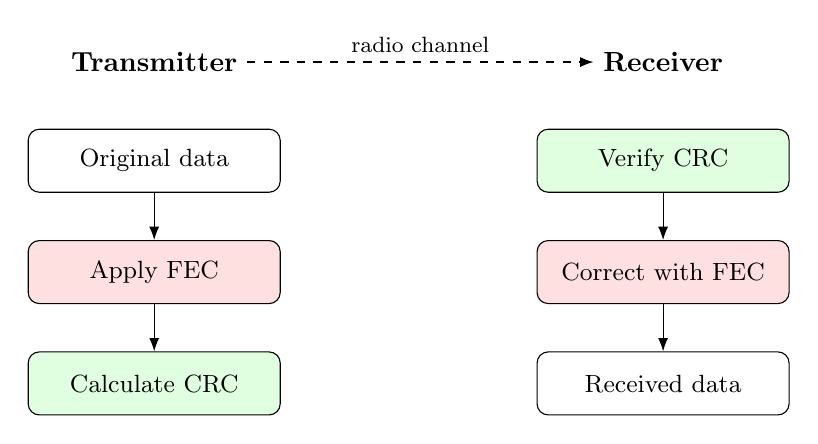
\begin{tikzpicture}[
  node distance=6mm,
  box/.style={draw,rounded corners,minimum width=3.2cm,minimum height=8mm,align=center,font=\small},
  hdr/.style={font=\bfseries},
]
\node[hdr] (txhdr) {Transmitter};
\node[box,below=of txhdr,fill=white] (tx1) {Original data};
\node[box,below=of tx1,fill=red!12] (tx2) {Apply FEC};
\node[box,below=of tx2,fill=green!12] (tx3) {Calculate CRC};

\node[hdr,right=4.4cm of txhdr] (rxhdr) {Receiver};
\node[box,below=of rxhdr,fill=green!12] (rx1) {Verify CRC};
\node[box,below=of rx1,fill=red!12] (rx2) {Correct with FEC};
\node[box,below=of rx2,fill=white] (rx3) {Received data};

\draw[-{Latex}] (tx1) -- (tx2);
\draw[-{Latex}] (tx2) -- (tx3);
\draw[-{Latex}] (rx1) -- (rx2);
\draw[-{Latex}] (rx2) -- (rx3);
\draw[-{Latex},dashed] (txhdr.east) -- node[above,font=\footnotesize]{radio channel} (rxhdr.west);
\end{tikzpicture}
\caption{Error detection (CRC) vs.\ forward error correction (FEC) in a
digital transmission chain.}
\end{figure}

\section{The Basic Problem}

A block of $k$ information bits, transmitted over a noisy channel, may
arrive with one or more bits flipped. Without any additional structure,
the receiver has no way to know this happened --- an altered but
still-valid-looking bit pattern is simply accepted as correct. Error
control techniques add carefully structured \textbf{redundant} bits to
the transmitted data specifically so the receiver can recognize (and, in
some schemes, correct) errors.

\section{Cyclic Redundancy Check (CRC)}

A \textbf{cyclic redundancy check} is an error-\emph{detection} (not
correction) scheme. The transmitter treats the data block as a large
binary number, divides it (using a special binary polynomial division,
modulo 2) by a fixed \textbf{generator polynomial}, and appends the
remainder --- the \textbf{CRC checksum} --- to the transmitted data. The
receiver performs the same division on the received data (including the
appended checksum) and checks whether the remainder is zero: if not, at
least one bit was altered in transit, and the receiver knows to discard
the block or request retransmission.

\begin{keyidea}
CRC is extremely effective at \emph{detecting} that an error occurred
(essentially guaranteed to catch any single-bit or short burst error,
and to catch the vast majority of longer or multiple-bit error
patterns, depending on the generator polynomial's length), but on its
own gives no way to determine \emph{which} bit was wrong, and therefore
no way to fix it. CRC-protected protocols typically respond to a failed
check by requesting a retransmission (an \textbf{automatic repeat
request}, ARQ) rather than attempting a repair.
\end{keyidea}

CRC is used throughout amateur digital communications: packet radio
(AX.25) frames include a CRC (technically an FCS, frame check sequence)
to catch corrupted packets; many file transfer and digital mode
protocols use CRC in a similar role.

\section{Forward Error Correction (FEC)}

\textbf{Forward error correction} takes a different, more ambitious
approach: it adds redundancy structured so that the receiver can
\emph{correct} at least some error patterns without needing any
retransmission at all --- valuable on links (satellite, weak-signal HF,
one-way beacon or telemetry transmissions) where requesting a repeat is
slow, expensive, or simply impossible.

\subsection{A Simple Example: The Repetition Code}

The simplest possible FEC scheme repeats each bit multiple times (e.g.,
three times: $0 \to 000$, $1 \to 111$) and uses \textbf{majority voting}
at the receiver to decide the original bit, correcting any single-bit
error within each group of three at the cost of tripling the
transmitted data. This illustrates the fundamental FEC trade-off in its
simplest form: \textbf{more redundancy buys more error-correcting
capability, at the direct cost of reduced information throughput for a
given channel bandwidth}.

\subsection{Practical FEC Codes}

Real FEC systems use far more efficient (less redundant, for the same
correcting power) mathematical structures than simple repetition:

\begin{itemize}
\item \textbf{Block codes} (Hamming, Reed--Solomon, BCH): operate on
fixed-size blocks of data, adding a calculated set of parity/check
symbols; Reed--Solomon codes are particularly good at correcting
\textbf{burst errors} (many consecutive bits corrupted together, typical
of fading and impulse noise) and are used in satellite telemetry and
digital broadcast standards.
\item \textbf{Convolutional codes}: encode a continuous stream of data
using a sliding-window structure, decoded with algorithms such as the
\textbf{Viterbi algorithm}; well suited to the continuously varying
noise conditions typical of a real radio channel, and long used in
satellite and deep-space communication.
\item \textbf{Low-density parity-check (LDPC) codes} and modern
\textbf{turbo codes}: iteratively decoded codes that approach the
theoretical (Shannon) limit of channel capacity very closely; used in
recent weak-signal amateur digital modes and modern satellite/deep-space
links.
\end{itemize}

\begin{keyidea}[Why weak-signal digital modes decode below the noise floor]
Modern weak-signal amateur digital modes (Chapter~\ref{ch:digital-modes})
combine strong FEC coding with narrow bandwidth and long averaging
(integration) times to reliably decode signals that are, by ear,
completely inaudible in the noise --- often 10--20\,dB below the noise
floor. The FEC code does not create information out of nothing; rather,
it lets the decoder use redundancy spread across the whole transmitted
block to statistically reconstruct the most likely original message
even when individual symbols are severely corrupted by noise.
\end{keyidea}

\section{Combining CRC and FEC}

Many real protocols use both techniques together: FEC coding to correct
the errors it can, followed by a CRC check on the FEC-decoded output to
catch (and flag or reject) any errors that were too severe for the FEC
to fix. This layered approach --- correct what you can, detect what you
cannot correct so bad data is never silently accepted as good --- is the
standard architecture for robust digital data links, including many
amateur satellite and digital-mode protocols.

\section{Automatic Repeat Request (ARQ)}

Where a return channel exists, error \emph{detection} (CRC) can be
combined with automatic retransmission: the receiver acknowledges
correctly received blocks and requests retransmission of blocks that
fail their CRC check. \textbf{ARQ} protocols (used in amateur packet
radio, Winlink, and many other bidirectional digital modes) trade
throughput and latency (a corrupted block must be resent, taking extra
time) for a very high assurance of eventually delivering error-free
data, in contrast to pure FEC, which trades bandwidth for correcting
errors without any retransmission delay but cannot guarantee a
perfect result on a very poor link.

\begin{quickreview}
\item CRC detects (but does not correct) errors by comparing a
transmitted and recomputed checksum; failed checks typically trigger a
retransmission request (ARQ).
\item FEC adds structured redundancy that lets the receiver correct
certain error patterns without retransmission, at the cost of reduced
raw throughput.
\item Block codes (Reed--Solomon, Hamming), convolutional codes, and
modern LDPC/turbo codes are the main practical FEC families, each suited
to different error patterns (burst vs.\ random) and decoding complexity
budgets.
\item Strong FEC plus narrow bandwidth and long integration time lets
modern digital modes decode signals well below the audible noise floor.
\item CRC and FEC are frequently combined: FEC corrects what it can,
CRC flags what remains uncorrected.
\end{quickreview}

\begin{practiceproblems}
\item Explain the key functional difference between error
\emph{detection} and error \emph{correction}.
\item A simple triple-repetition FEC code receives the group ``101''
for a transmitted single bit. Using majority voting, what was the
original bit most likely to have been, and can you be certain?
\item Explain why Reed--Solomon-style codes are particularly well suited
to correcting burst errors caused by fading, compared to a code
optimized only for isolated single-bit errors.
\item Explain why a protocol might use both FEC and CRC together rather
than relying on FEC alone.
\item Explain, at a conceptual level (no equations required), how
combining strong FEC with a very narrow receive bandwidth and long
averaging time allows some digital modes to decode signals inaudible to
the human ear.
\end{practiceproblems}


\part{Antennas, Transmission Lines, and Propagation}
\chapter{Transmission Lines and Standing Wave Ratio}
\label{ch:transmission-lines}

A \textbf{transmission line} (coaxial cable, open-wire ladder line,
twisted pair) carries RF energy from a transmitter to an antenna, or
from an antenna to a receiver, with as little loss and distortion as
possible. Unlike the DC and low-frequency AC circuits of earlier
chapters, a transmission line's physical length is often a significant
fraction of the signal's wavelength, and its behavior must be analyzed
as a distributed, wave-carrying system rather than a simple two-terminal
lumped circuit.

\section{Characteristic Impedance}

Every transmission line has a \textbf{characteristic impedance} $Z_0$,
determined entirely by its physical geometry (conductor spacing,
diameter, dielectric) and, for an ideal lossless line, independent of
its length or the frequency of the signal on it:
\[
Z_0 = \sqrt{\frac{L'}{C'}}
\]
where $L'$ and $C'$ are the line's inductance and capacitance \emph{per
unit length}. Common amateur coaxial cable is manufactured to standard
values of 50\,$\Omega$ (the overwhelming standard for amateur HF/VHF/UHF
work) or 75\,$\Omega$ (common in broadcast and video applications);
open-wire ladder line is typically 300--600\,$\Omega$.

\begin{keyidea}
$Z_0$ is \emph{not} something you measure with an ohmmeter across a
disconnected line's ends (a long line will simply read as an open or
short circuit depending on its length relative to a wavelength) --- it
describes the impedance a wave experiences while traveling \emph{along}
the line, and only becomes directly relevant once the line is driving a
load and carrying a traveling wave.
\end{keyidea}

\section{Matched vs.\ Mismatched Loads}

When a transmission line is terminated in a load whose impedance exactly
equals $Z_0$, all of the power traveling down the line is absorbed by
the load; no energy is reflected. This is a \textbf{matched} condition.
If the load impedance $Z_L$ differs from $Z_0$, some of the incident
power is reflected back toward the source, creating a second wave
traveling in the opposite direction. The interference between the
forward (incident) and reflected waves creates a \textbf{standing
wave} pattern of voltage and current along the line.

\section{Reflection Coefficient and SWR}

The fraction of voltage reflected is the \textbf{reflection
coefficient}, $\Gamma$ (Greek capital gamma), a complex number in
general but often quoted by magnitude:
\[
\boxed{\Gamma = \frac{Z_L - Z_0}{Z_L + Z_0}}
\]
$\Gamma = 0$ for a perfectly matched load; $|\Gamma| = 1$ for a
completely reactive/open/short load (total reflection, no power
absorbed).

The \textbf{standing wave ratio (SWR)}, the ratio of the standing wave
pattern's maximum voltage to its minimum voltage along the line, is
related directly to $|\Gamma|$:
\[
\boxed{\text{SWR} = \frac{V_{\max}}{V_{\min}} = \frac{1+|\Gamma|}{1-|\Gamma|}}
\]
SWR is always $\geq 1$, with 1{:}1 representing a perfect match. Because
it depends only on $|\Gamma|$, SWR (unlike $\Gamma$ itself) carries no
information about the \emph{phase} of the mismatch --- only its
severity.

\begin{examplebox}[SWR from a load mismatch]
A 50\,$\Omega$ line is terminated in a 75\,$\Omega$ resistive load.
Find $\Gamma$ and the SWR.

\emph{Solution.}
\[
\Gamma = \frac{75-50}{75+50} = \frac{25}{125} = 0.2, \qquad
\text{SWR} = \frac{1+0.2}{1-0.2} = \frac{1.2}{0.8} = 1.5.
\]
A 1.5:1 SWR, generally considered a mild, acceptable mismatch.
\end{examplebox}

\section{Power Reflected}

The fraction of incident power that is reflected (rather than
delivered to the load) is $|\Gamma|^2$:
\[
\frac{P_{\text{reflected}}}{P_{\text{forward}}} = |\Gamma|^2.
\]

\begin{examplebox}[Power lost to reflection]
For the 1.5:1 SWR example above ($|\Gamma|=0.2$), find the fraction of
power reflected and the fraction delivered to the load.

\emph{Solution.}
\[
\frac{P_{\text{reflected}}}{P_{\text{forward}}} = 0.2^2 = 0.04\ (4\%), \qquad
\text{delivered} = 96\%.
\]
This illustrates why a modest 1.5:1 SWR is rarely a practical problem:
the actual power lost to reflection is small. Very high SWR (5:1 or
worse) reflects a much larger fraction of power and can additionally
stress transmitter output stages and increase line loss significantly.
\end{examplebox}

\section{Why High SWR Matters}

\begin{itemize}
\item \textbf{Transmitter stress}: many solid-state transmitters
automatically reduce power (``foldback'') or shut down when SWR exceeds
a safe limit, since a severely mismatched load can present the final
amplifier stage with voltage or current levels well outside its safe
operating range.
\item \textbf{Increased line loss}: standing waves increase the peak
current and voltage on the line relative to a matched condition,
increasing $I^2R$ and dielectric losses beyond the line's already
frequency-dependent matched-line loss --- the mismatch loss adds on top
of, and interacts with, the line's intrinsic loss.
\item \textbf{Voltage/current peaks}: at high SWR, the standing wave's
voltage and current maxima can be large enough to cause arcing or
component stress at those points along the line, even if the average
power is modest.
\end{itemize}

\begin{safetynote}
Very high SWR at significant power levels can generate dangerously high
RF voltages at points along a feedline or at an antenna feedpoint,
particularly with unterminated or badly damaged coaxial lines. Address
high SWR readings before operating at higher power levels.
\end{safetynote}

\section{Impedance Along a Mismatched Line}

For a lossless line of length $\ell$ and characteristic impedance
$Z_0$, terminated in load $Z_L$, the impedance seen looking into the
line varies periodically with distance from the load, repeating every
half wavelength:
\[
Z_{\text{in}} = Z_0\,\frac{Z_L + jZ_0\tan(\beta\ell)}{Z_0 + jZ_L\tan(\beta\ell)}, \qquad \beta = \frac{2\pi}{\lambda}.
\]
Two special cases are worth knowing without the full formula:

\begin{itemize}
\item A line exactly \textbf{one-half wavelength} (or any integer
multiple) long repeats the load impedance at its input, regardless of
$Z_0$ --- useful for relocating a matched (or known) impedance to a more
convenient physical location.
\item A line exactly \textbf{one-quarter wavelength} long acts as an
impedance \textbf{inverter/transformer}: $Z_{\text{in}} = Z_0^2/Z_L$.
This \textbf{quarter-wave transformer} principle is widely used to
match a real, resistive antenna feedpoint impedance to a different
feedline impedance using a length of line with an intermediate
characteristic impedance, $Z_0 = \sqrt{Z_{\text{in}}Z_L}$.
\end{itemize}

\section{Line Loss}

Real transmission lines dissipate some power even when perfectly
matched, due to conductor resistance (worse at higher frequency because
of the \textbf{skin effect}, Chapter~\ref{ch:inductors}) and dielectric
loss in the insulating material. Manufacturers publish matched-line
loss in dB per 100\,m (or 100\,ft) at various frequencies; loss
increases with frequency and, for a fixed cable type, with distance.
Mismatch (SWR $>1$) adds additional loss on top of this intrinsic
matched-line loss, an effect that becomes more significant as intrinsic
cable loss increases (which is one reason high SWR is more consequential
on a long run of lossy cable than on a short run of low-loss line).

\begin{quickreview}
\item Characteristic impedance $Z_0 = \sqrt{L'/C'}$ depends on line
geometry, not length or (ideally) frequency.
\item $\Gamma = (Z_L-Z_0)/(Z_L+Z_0)$; SWR $=(1+|\Gamma|)/(1-|\Gamma|)$;
reflected power fraction $=|\Gamma|^2$.
\item High SWR can stress transmitters, increase line loss, and produce
dangerous voltage/current peaks at significant power.
\item A half-wavelength line repeats the load impedance; a
quarter-wavelength line transforms impedance as
$Z_{\text{in}} = Z_0^2/Z_L$.
\item Real lines have intrinsic matched loss (worse at higher
frequency); mismatch adds further loss on top of this.
\end{quickreview}

\begin{practiceproblems}
\item A 50\,$\Omega$ line feeds a purely resistive 100\,$\Omega$ load.
Find $\Gamma$ and SWR.
\item For an SWR of 3:1, find $|\Gamma|$ and the fraction of power
reflected.
\item Find the characteristic impedance of a quarter-wave matching
section needed to match a 50\,$\Omega$ line to a 200\,$\Omega$ antenna
feedpoint.
\item Explain why a transmitter's automatic power foldback at high SWR
is a protective feature rather than a fault.
\item A 1:1 SWR is measured at the transmitter end of a long, lossy
feedline. Does this guarantee the antenna itself is well matched?
Explain, considering line loss.
\end{practiceproblems}

\chapter{Antenna Fundamentals and Common Designs}
\label{ch:antennas}

An antenna is the transducer between guided energy on a transmission
line and free-space electromagnetic waves (Chapter~\ref{ch:fields}),
working identically (by reciprocity) whether transmitting or receiving.
This chapter covers the core parameters used to describe any antenna,
then surveys the designs an amateur is most likely to build or use.

\section{Radiation: Why an Oscillating Charge Radiates}

An accelerating (including oscillating) electric charge radiates
electromagnetic energy. A current-carrying conductor driven at radio
frequency has continuously accelerating charge carriers, and therefore
radiates --- but efficient radiation requires the conductor's length to
be comparable to the signal's wavelength (Chapter~\ref{ch:fields}, $c =
f\lambda$); a conductor much shorter than a wavelength radiates very
inefficiently, which is why antenna dimensions scale directly with
operating wavelength.

\section{The Half-Wave Dipole}

\bookfig[0.55]{antena_dipolo.png}{A center-fed half-wave dipole antenna.}

The \textbf{half-wave dipole} --- two straight conductors, each
approximately a quarter-wavelength long, fed at the center --- is the
fundamental reference antenna against which most others are compared.
Its resonant length, accounting for the practical fact that RF
propagates slightly slower along a real (finite-diameter) wire than in
free space (the \textbf{velocity factor} or ``end effect''), is
approximately
\[
\boxed{\ell_{\text{ft}} = \frac{468}{f_{\text{MHz}}}} \qquad \text{or equivalently} \qquad
\ell_{\text{m}} \approx \frac{143}{f_{\text{MHz}}}
\]
for total dipole length. (The free-space half-wavelength would be
$\ell = c/(2f) = 150/f_{\text{MHz}}$ metres; the shortening factor,
roughly 0.95, accounts for end effect in typical thin-wire
construction.)

\begin{examplebox}[Dipole length]
Find the total length of a half-wave dipole for 7.100\,MHz.

\emph{Solution.}
\[
\ell_{\text{m}} \approx \frac{143}{7.100} \approx 20.1\,\text{m}.
\]
Each leg is therefore approximately 10.1\,m.
\end{examplebox}

A resonant half-wave dipole in free space presents a feedpoint
impedance of approximately $73\,\Omega$ (resistive, at resonance),
reasonably close to standard 50\,$\Omega$ coax, though height above
ground and surroundings shift this value somewhat in practice. A dipole
fed at its center is inherently a \textbf{balanced} load and should be
fed through a balun (Chapter~\ref{ch:transformers}) if connected to
unbalanced coaxial cable, to avoid feedline radiation and pattern
distortion.

\section{Radiation Pattern, Gain, and Directivity}

An antenna's \textbf{radiation pattern} describes how strongly it
radiates as a function of direction. Even the simplest dipole is not
omnidirectional in three dimensions: it radiates a figure-eight pattern
broadside to the wire (maximum) and radiates essentially nothing off the
ends of the wire (nulls).

\textbf{Directivity} and \textbf{gain} quantify how much an antenna
concentrates radiation in its favored direction(s) compared to a
reference. Gain, expressed in \textbf{dBi} (relative to a theoretical
isotropic radiator) or \textbf{dBd} (relative to a reference dipole),
was defined precisely in Chapter~\ref{ch:decibels}; a real dipole has
about 2.15\,dBi (0\,dBd) of gain in its favored broadside directions,
simply from concentrating energy away from the (nulled) end directions
rather than spreading it equally in all directions like a true
isotropic source.

\begin{keyidea}[Gain is a trade, not free energy]
An antenna cannot amplify signal power --- gain in one direction is
always achieved by concentrating radiation that would otherwise have
gone elsewhere, not by adding energy. A high-gain directional antenna
therefore radiates \emph{less} in directions away from its main lobe
than an isotropic radiator would, even as it radiates significantly
\emph{more} in its favored direction.
\end{keyidea}

\section{Antenna Efficiency and Losses}

\bookfig[0.55]{antena_eficiencia.png}{Antenna efficiency: radiated
power vs.\ power lost to resistive and ground losses.}

Real antennas dissipate some power as heat rather than radiating it all,
due to conductor resistance, loading-coil losses, and losses in nearby
lossy ground or objects. \textbf{Radiation efficiency} is
\[
\eta = \frac{R_{\text{rad}}}{R_{\text{rad}}+R_{\text{loss}}} \times 100\%
\]
where $R_{\text{rad}}$ is the antenna's \textbf{radiation resistance}
(the equivalent resistance that would dissipate the same power as is
actually radiated) and $R_{\text{loss}}$ lumps together all real
resistive losses. Electrically short antennas (loaded verticals and
mobile whips well under a quarter-wavelength, for instance) tend to have
low radiation resistance, making loss resistance a proportionally larger
fraction of the total and efficiency correspondingly poorer --- a key
reason full-size or close-to-full-size antennas generally outperform
heavily shortened/loaded designs when space permits.

\section{Polarization and Ground Effects}

An antenna's orientation sets its \textbf{polarization}
(Chapter~\ref{ch:fields}): a horizontal dipole radiates
horizontally polarized waves; a vertical antenna radiates vertically
polarized waves. Ground reflections interact strongly with a nearby
antenna, modifying both its feedpoint impedance and its radiation
pattern (particularly the low-angle performance important for
long-distance HF propagation, Chapter~\ref{ch:propagation}); antenna
height above ground, in wavelengths, is therefore a major practical
design variable, not just an installation convenience.

\section{The Yagi--Uda Antenna}

\bookfig[0.6]{antena_yagi.png}{A Yagi--Uda beam antenna: driven
element, reflector, and directors.}

The \textbf{Yagi--Uda} antenna (commonly just ``Yagi''), invented by
Shintaro Uda and popularized by Hidetsugu Yagi in the 1920s, achieves
significant directional gain from a single driven half-wave dipole
element by adding nearby \textbf{parasitic elements}: a slightly longer
\textbf{reflector} behind the driven element and one or more slightly
shorter \textbf{directors} in front of it. These parasitic elements are
not directly fed; they are excited by mutual coupling with the driven
element's near field, and their carefully tuned length and spacing
cause constructive interference in the forward direction and
destructive interference to the rear, producing a directional beam
pattern with useful gain (typically 6--15\,dBi depending on the number
of elements and boom length) and a front-to-back ratio that helps reject
interference and noise arriving from behind the antenna.

\section{Ground-Plane and Vertical Antennas}

\bookfig[0.5]{antena_ground_plane.png}{A quarter-wave ground-plane
vertical antenna with radial elements.}

A \textbf{ground-plane vertical} uses a quarter-wave vertical radiator
fed against a set of radial elements (or an actual conductive ground
plane) that serve as the antenna's ``other half,'' effectively forming
half of a dipole with an electrical mirror image below the
feedpoint. Feedpoint impedance for an ideal quarter-wave vertical over a
perfect ground plane is approximately $36\,\Omega$ (roughly half the
dipole's $73\,\Omega$, consistent with the mirror-image picture).
Verticals radiate omnidirectionally in azimuth (all compass directions
equally) with vertical polarization, and --- with a low radiation angle
particularly useful for DX contacts --- are popular where a horizontal
antenna large enough for the operating band is impractical, at the cost
of typically needing an effective radial/ground system to perform well.

\section{Loop Antennas}

\bookfig[0.5]{antena_loop_magnetica.jpg}{A small transmitting magnetic
loop antenna.}

A \textbf{loop antenna} forms a closed (or nearly closed) conductive
loop. \textbf{Full-size loops} (a wavelength or more in circumference)
behave broadly like a folded dipole variant with useful gain and
different polarization/pattern characteristics depending on
orientation. \textbf{Small (magnetic) loops}, with circumference well
under a wavelength, are physically compact and couple predominantly to
the magnetic near-field component; they achieve resonance using a
high-voltage tuning capacitor across the loop and, despite modest
radiation efficiency for their small size, are valued for
space-constrained installations and for a naturally narrow bandwidth
that provides useful front-end selectivity even before a receiver's own
filtering.

\section{Multiband and Wire Antenna Techniques}

\begin{figure}[H]
\centering
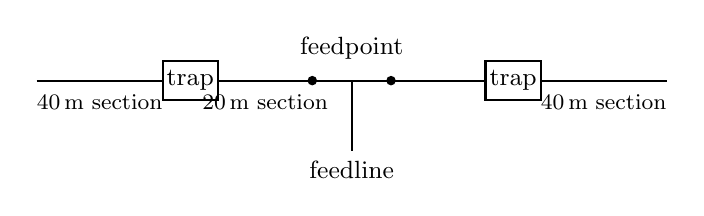
\begin{tikzpicture}[scale=1,every node/.style={font=\small}]
\draw[thick] (0,0) -- (1.6,0);
\draw[thick] (1.6,-0.25) rectangle (2.3,0.25) node[midway]{trap};
\draw[thick] (2.3,0) -- (3.5,0);
\filldraw (3.5,0) circle (1.5pt);
\draw[thick] (3.5,0) -- (4.5,0);
\filldraw (4.5,0) circle (1.5pt);
\draw[thick] (4.5,0) -- (5.7,0);
\draw[thick] (5.7,-0.25) rectangle (6.4,0.25) node[midway]{trap};
\draw[thick] (6.4,0) -- (8,0);
\draw[thick] (4,0) -- (4,-0.9);
\node[below] at (4,-0.9) {feedline};
\node[below,align=center] at (0.8,-0.05) {\footnotesize 40\,m section};
\node[below,align=center] at (2.9,-0.05) {\footnotesize 20\,m section};
\node[below,align=center] at (7.2,-0.05) {\footnotesize 40\,m section};
\node[above] at (4,0.15) {feedpoint};
\end{tikzpicture}
\caption{A trap dipole: LC traps present a high impedance at their
design frequency, electrically shortening the antenna so a single wire
resonates on more than one band.}
\end{figure}

\begin{itemize}
\item \textbf{Trap dipoles/verticals}: parallel LC resonant circuits
(\textbf{traps}, Chapter~\ref{ch:rlc-resonance}) inserted along the
antenna element present a high impedance (effectively an open circuit,
electrically shortening the antenna) at their design frequency, letting
a single physical antenna present resonant electrical lengths on
several different bands.
\item \textbf{End-fed half-wave (EFHW) antennas}: a half-wave wire fed
at (or very near) one end, where feedpoint impedance is very high
(thousands of ohms) rather than the ${\sim}73\,\Omega$ of a center-fed
dipole; a purpose-built impedance-matching transformer converts this
high impedance down to $50\,\Omega$, letting the antenna be fed
conveniently from one end rather than requiring center support.
\item \textbf{Folded dipoles}: a dipole with a second parallel
conductor connecting its two ends, raising feedpoint impedance
(approximately $4\times$ a plain dipole's, or about $280$--$300\,\Omega$
for a simple two-wire fold) and providing a somewhat broader bandwidth
--- the classic feed for 300\,$\Omega$ balanced television ribbon line
and folded-element Yagi driven elements.
\end{itemize}

\begin{figure}[H]
\centering
\begin{tikzpicture}[scale=1,every node/.style={font=\small}]
\draw[thick] (0,0) -- (6.4,2.1);
\node[above] at (3.2,1.05) {half-wave wire ($\approx\lambda/2$)};
\draw[thick] (6.4,2.1) circle (2.5pt);
\node[above right] at (6.4,2.1) {end support/insulator};
\draw[thick] (-0.3,-0.4) rectangle (0.5,0.2);
\node[left] at (-0.35,-0.1) {matching transformer};
\draw[thick] (0.1,-0.4) -- (0.1,-1.1);
\node[below] at (0.1,-1.1) {\small 50\,$\Omega$ coax to radio};
\end{tikzpicture}
\caption{An end-fed half-wave (EFHW) antenna. A step-up impedance
transformer (typically 49:1 or 64:1) matches the wire's high end-feed
impedance down to 50\,$\Omega$.}
\end{figure}

\section{Antenna Bandwidth}

\bookfig[0.65]{antena_bandas.png}{Typical amateur HF antenna bandwidth
across several bands.}

An antenna's usable \textbf{bandwidth} (the frequency range over which
its feedpoint impedance stays reasonably close to the feedline's
characteristic impedance, typically judged by SWR) depends on the
antenna's own effective $Q$ (Chapter~\ref{ch:rlc-resonance}): thicker
conductors and lower operating $Q$ generally give wider bandwidth,
which is why a fan dipole, thick aluminum Yagi element, or cage dipole
often covers more of a band comfortably than a thin, single wire of the
same nominal design.

\begin{quickreview}
\item An antenna radiates because it carries oscillating (accelerating)
charge; efficient radiation needs dimensions comparable to a wavelength.
\item Half-wave dipole length (m) $\approx 143/f_{\text{MHz}}$;
free-space feedpoint impedance $\approx 73\,\Omega$.
\item Gain (dBi/dBd) describes concentration of radiation in a favored
direction, not added total power; efficiency $\eta =
R_{\text{rad}}/(R_{\text{rad}}+R_{\text{loss}})$.
\item Yagi--Uda antennas use parasitic reflector/director elements
around one driven element to achieve directional gain.
\item Verticals/ground-planes give omnidirectional, low-angle,
vertically polarized radiation; loops, traps, EFHW, and folded-dipole
techniques address space, multiband, and feed-impedance needs.
\end{quickreview}

\begin{practiceproblems}
\item Find the total length of a half-wave dipole for 21.200\,MHz.
\item A Yagi has 10\,dBi of gain. Express this in dBd.
\item Explain why an electrically short, heavily loaded mobile whip
antenna typically has lower efficiency than a full-size dipole on the
same band.
\item Explain, in terms of the mirror-image picture, why a quarter-wave
ground-plane vertical's feedpoint impedance is roughly half that of a
half-wave dipole.
\item Explain the practical purpose of a matching transformer on an
end-fed half-wave antenna, given that a half-wave wire's end-fed
impedance is very high rather than close to 50\,$\Omega$.
\end{practiceproblems}

\chapter{Radio Wave Propagation}
\label{ch:propagation}

How a radio signal gets from a transmitting antenna to a receiving
antenna, hundreds or thousands of kilometres away, depends on frequency,
time of day, season, solar activity, and geography. This chapter surveys
the main propagation mechanisms an amateur exploits across the HF, VHF,
UHF, and microwave amateur bands.

\section{The Ground Wave}

At lower frequencies (roughly below a few MHz), a vertically polarized
wave can travel along the Earth's curved surface for a considerable
distance as a \textbf{ground wave} (or \textbf{surface wave}), guided
partly by the interaction between the wave and the conductive ground.
Ground-wave range is limited by ground conductivity (seawater performs
far better than dry rocky or sandy soil) and increases at lower
frequency; it is a minor factor for most HF amateur bands but is the
dominant propagation mode for AM broadcast and some maritime/beacon
services at lower frequencies.

\section{Line-of-Sight and the Radio Horizon}

At VHF, UHF, and microwave frequencies, propagation is normally
\textbf{line-of-sight}: the direct wave travels essentially in a
straight line, blocked by the curvature of the Earth and by terrain
obstructions. Because the atmosphere's refractive index normally
decreases slightly with height, radio waves bend (\textbf{refract})
gently downward, extending the effective \textbf{radio horizon} somewhat
beyond the optical horizon --- a commonly used approximation for the
radio horizon distance (in kilometres, with antenna height $h$ in
metres) is
\[
d_{\text{km}} \approx 4.12\sqrt{h_{\text{m}}}
\]
applied to each end of the path and summed, which is why raising a
VHF/UHF antenna (or operating from a hilltop) so directly and
dramatically increases usable range.

\subsection{Tropospheric Effects}

Under certain weather conditions, temperature and humidity gradients in
the lower atmosphere (\textbf{troposphere}) create layers where the
refractive index changes more sharply than usual, bending
(\textbf{tropospheric ducting} or simple \textbf{tropo enhancement}) VHF
and UHF signals well beyond the normal radio horizon --- sometimes
hundreds of kilometres --- along stable high-pressure weather boundaries
or temperature inversions. \textbf{Tropospheric scatter}, a weaker but
more consistently available mechanism, allows some signal energy to
scatter forward off small-scale turbulence in the troposphere even
without a defined duct.

\section{The Ionosphere and Skywave Propagation}

The \textbf{ionosphere} is a region of the upper atmosphere
(approximately 60--1000\,km altitude) where solar ultraviolet and X-ray
radiation ionizes atmospheric gases, creating layers of free electrons
capable of refracting (and, at a steep enough angle or low enough
frequency, fully reflecting) radio waves back toward Earth. This
\textbf{skywave} propagation is what makes long-distance (``DX'') HF
communication possible without a chain of relay stations, by bouncing a
signal off the ionosphere and back down to a distant receiver --
potentially over several successive ``hops.''

\subsection{Ionospheric Layers}

\begin{itemize}
\item \textbf{D layer} (${\sim}60$--90\,km): forms only in daylight;
does not refract HF signals back to Earth but does \emph{absorb} them,
particularly at lower HF frequencies --- the main reason low HF bands
(80\,m, 40\,m) are noticeably ``quieter'' but shorter-range for DX
during the day and open up dramatically for longer-distance
propagation after D-layer ionization decays at night.
\item \textbf{E layer} (${\sim}90$--150\,km): present mainly in
daylight, refracts lower/mid HF frequencies and supports the anomalous,
short-lived \textbf{sporadic-E} propagation discussed below.
\item \textbf{F layer} (splitting into \textbf{F1} and \textbf{F2} in
daylight, recombining into a single F layer at night, roughly
150--500\,km): the primary layer responsible for long-distance HF
skywave propagation, with the F2 layer's height and ionization density
--- strongly dependent on solar activity --- setting the
\textbf{maximum usable frequency (MUF)} for a given path on a given day.
\end{itemize}

\subsection{Critical Frequency and MUF}

For a signal transmitted straight up, the highest frequency the
ionosphere will still reflect back down is the \textbf{critical
frequency}, $f_c$. For a signal transmitted at an oblique angle
(the normal case for a real communication path), a higher frequency
can still be refracted back to Earth --- the \textbf{maximum usable
frequency} for that specific path, related to the critical frequency and
the wave's incidence angle $\theta$ (measured from vertical) by the
\textbf{secant law}:
\[
\boxed{\text{MUF} = f_c \sec(\theta)}
\]
Operating above the MUF for a given path, the signal passes through the
ionosphere into space rather than being returned to Earth. Because lower
launch angles (more oblique, larger $\theta$) permit a higher MUF, DX
contacts over very long paths are often possible at frequencies that
would not support shorter, steeper-angle paths at the same time.

\begin{keyidea}[LUF, MUF, and the usable window]
Below a \textbf{lowest usable frequency (LUF)}, D-layer absorption (and
increasing atmospheric/man-made noise at lower frequencies) makes a
signal too weak to be useful even if the ionosphere would otherwise
support the path; above the MUF, the signal is not returned to Earth at
all. Real-world HF operation lives in the changing window between these
two limits, which is why band selection ``for the conditions'' is such
a core operating skill --- and why real-time MUF/LUF prediction tools
and propagation beacons are widely used by serious HF operators.
\end{keyidea}

\section{The Solar Cycle and Space Weather}

Ionization of the F2 layer depends strongly on solar ultraviolet
output, which varies on an approximately \textbf{11-year solar cycle} of
rising and falling sunspot activity. Higher sunspot numbers generally
mean a denser, higher F2 layer and a correspondingly higher MUF,
supporting DX propagation on higher HF bands (15\,m, 12\,m, 10\,m) that
may be largely closed during solar minimum. Solar flares and coronal
mass ejections can also cause sudden, disruptive space-weather events:

\begin{itemize}
\item A \textbf{sudden ionospheric disturbance (SID)}, triggered by a
solar flare's X-ray flux, causes a rapid increase in D-layer ionization
and a corresponding \textbf{HF radio blackout} on the sunlit side of
Earth, lasting from minutes to a few hours.
\item A \textbf{geomagnetic storm}, triggered by a coronal mass
ejection reaching Earth's magnetosphere, disturbs the ionosphere over a
longer period (a day or more), variably degrading HF propagation while
sometimes \emph{enhancing} high-latitude VHF/UHF propagation via aurora.
\end{itemize}

\section{Sporadic-E}

\textbf{Sporadic-E} propagation results from dense, patchy, short-lived
clouds of ionization in the E layer (mechanism not fully understood, but
statistically linked to season --- most common in late spring/early
summer in each hemisphere --- and to wind shear in the upper
atmosphere). It can support surprisingly strong single- or
multi-hop propagation on the upper HF bands and, notably, on the lower
VHF bands (6\,m and, less commonly, 2\,m) that are normally limited to
line-of-sight --- producing some of the most exciting unpredictable
VHF DX openings available to an amateur.

\section{Meteor Scatter and Auroral Propagation}

\begin{itemize}
\item \textbf{Meteor scatter}: the brief ionized trail left by a meteor
burning up in the upper atmosphere can reflect VHF signals for a
fraction of a second to a few seconds, long enough (especially with
digital modes designed for very short contacts) to complete brief
contacts over 1000--2000\,km paths, enhanced during annual meteor
showers.
\item \textbf{Auroral propagation}: during geomagnetic disturbances,
VHF/UHF signals can scatter off ionization associated with the aurora,
typically producing a characteristic rasping, Doppler-smeared signal
quality, mainly usable for paths oriented toward the auroral region at
higher latitudes.
\end{itemize}

\section{Greyline Propagation}

The \textbf{greyline} (or \textbf{terminator}) is the band of twilight
circling the Earth between day and night. Along the greyline, the D
layer on the sunset/sunrise side has largely decayed (reducing
absorption) while the F layer, which decays more slowly after sunset,
remains sufficiently ionized to support propagation --- a favorable
combination that experienced HF operators specifically exploit for
long-path and unusual DX openings around their local sunrise and
sunset.

\section{Multipath, Fading, and Doppler Effects}

A received signal often arrives via more than one path simultaneously
(different ionospheric hops, ground wave plus skywave, or multiple
ionospheric layers at once), each with a slightly different path length
and therefore a different arrival phase. The combination of these
paths, constantly shifting as the ionosphere changes, produces
\textbf{fading} --- and, over sufficiently different path lengths,
measurable time-domain echo or \textbf{Doppler}-related frequency
smearing, both of particular relevance to digital mode performance
(Chapter~\ref{ch:digital-modes}) and to precise frequency measurement.

\begin{quickreview}
\item Ground wave (low HF/MF, vertical polarization) and line-of-sight
plus tropospheric effects (VHF/UHF/microwave) dominate at those
frequency extremes; skywave dominates general-purpose HF DX.
\item Ionospheric D, E, and F layers absorb (D) or refract (E, F)
HF signals; the F2 layer sets the MUF for long-distance skywave paths,
MUF $= f_c\sec\theta$.
\item The solar cycle and space-weather events (SIDs, geomagnetic
storms) drive large day-to-day and year-to-year variation in HF
propagation.
\item Sporadic-E, meteor scatter, and auroral propagation are
anomalous mechanisms that can open otherwise line-of-sight-limited
VHF bands over much longer paths.
\item Greyline propagation exploits the favorable D-layer/F-layer
balance found along the day/night terminator.
\end{quickreview}

\begin{practiceproblems}
\item Estimate the radio horizon distance for a VHF station with a
30\,m antenna height, communicating with a station whose antenna is
10\,m high (sum both contributions).
\item A path has a critical frequency of 4\,MHz and an incidence angle
of $70\degree$ from vertical. Estimate the MUF for this path.
\item Explain why the 80\,m and 40\,m amateur bands are typically much
better for long-distance contacts at night than during the day.
\item Explain, qualitatively, why higher sunspot activity tends to
improve propagation on the higher HF bands (e.g., 10\,m) specifically.
\item Explain why meteor scatter contacts are typically brief and rely
on specialized digital modes rather than sustained voice conversation.
\end{practiceproblems}


\part{Operating Practice and the Amateur Service Worldwide}
\chapter{Becoming a Licensed Amateur: An International Overview}
\label{ch:becoming-a-ham}

Every country that permits amateur radio operates its own licensing
system, but nearly all of them share a common shape, because nearly all
of them are built around the same international framework. This chapter
explains that shared shape without attempting to describe any single
country's specific rules --- for those, always consult your own national
telecommunications regulator or IARU member society.

\section{Why Licensing Exists at All}

Amateur radio operators are granted access to shared, finite radio
spectrum and are permitted to transmit at power levels that can cause
real interference to other services (aviation, marine, emergency
communications, other amateurs) if used carelessly. Licensing exists to
verify, before granting that access, that an operator understands enough
electronics, radio theory, and operating procedure to use the privilege
responsibly --- which is precisely the material this book is designed to
teach.

\section{The International Framework}

\begin{keyidea}
Nearly every national licensing system sits underneath the same
international structure: the \textbf{International Telecommunication
Union (ITU)} allocates radio spectrum globally and divides the world
into three \textbf{ITU Regions} for band-planning purposes; the
\textbf{International Amateur Radio Union (IARU)} coordinates amateur
band planning and operating practice within that framework; and
\textbf{CEPT} (in Europe) and similar regional bodies elsewhere
facilitate reciprocal license recognition between member countries.
These bodies are covered in full in Chapter~\ref{ch:regulatory-bodies}.
\end{keyidea}

\section{Typical License Tiers}

Although the exact names, requirements, and privileges differ by
country, most administrations offer licensing in \textbf{progressive
tiers}, each unlocking greater operating privileges (more bands, higher
power, more modes) in exchange for demonstrating greater technical
knowledge. A common three-tier pattern, which this book's five parts are
loosely organized around, looks approximately like this:

\begin{center}
\renewcommand{\arraystretch}{1.3}
\begin{tabularx}{\linewidth}{@{}p{3.1cm} Y Y@{}}
\toprule
Typical tier & Typical exam scope & Typical privileges \\
\midrule
Entry-level (``Foundation,'' ``Novice,'' ``Technician'') &
Basic safety, regulations, and simple operating procedure; limited
electronics theory &
Limited bands and/or power, often VHF/UHF-focused; sometimes CW-only or
supervised HF access \\
Intermediate (``General,'' ``Class~2'') &
Adds AC theory, components, antennas, and propagation basics &
Wider HF band access, higher power limits \\
Full/Advanced (``Extra,'' ``Class~1,'' ``Full'') &
Adds active devices, filters, transmission line theory, and deeper
technical detail &
Full amateur band and power privileges available in that country \\
\bottomrule
\end{tabularx}
\end{center}

Some countries use two tiers, some four or five; some require a period
of experience or a practical assessment between tiers; some (though a
shrinking number worldwide) still require a Morse code proficiency
test for HF privileges. Always check your own regulator's current
requirements rather than assuming any particular country's structure.

\section{What Exams Actually Test}

Despite wide variation in format (multiple choice is most common
worldwide; some countries use written or oral components), amateur
radio exams overwhelmingly test the same underlying knowledge areas,
each of which maps directly onto a part of this book:

\begin{itemize}
\item \textbf{Basic electricity and electronics} (Ohm's law, power,
components, AC theory) --- Parts~I and~II of this book.
\item \textbf{RF theory} (resonance, filters, semiconductors, receivers,
modulation) --- Part~III.
\item \textbf{Antennas, feedlines, and propagation} --- Part~IV.
\item \textbf{Operating procedure and radio safety} --- Part~V.
\item \textbf{National regulations specific to your country}: band
plans, power limits, callsign format, station identification
requirements, and the administrative process for obtaining and renewing
a license. \emph{This last category is intentionally not covered in
this book} and must be learned from your national regulator's own
official study materials.
\end{itemize}

\section{Practical Exam Preparation Advice}

\begin{examtip}
Most national exam question pools are published in advance, often with
the exact wording of every possible question. Working through the
official question pool for your specific country, alongside (not
instead of) understanding the underlying theory in this book, is by far
the most efficient way to prepare --- memorizing a question pool without
understanding the theory behind it leaves gaps that show up the moment a
real operating or troubleshooting situation differs even slightly from
a memorized question.
\end{examtip}

\begin{itemize}
\item Work practice questions from your own country's official or
widely used question pool.
\item Revisit the worked examples and practice problems in each chapter
of this book until the underlying calculation (not just the final
number) feels routine.
\item Use Appendix~A (formula reference) for rapid last-minute review,
but make sure you can also derive or explain \emph{why} each formula
works, not just recite it.
\item If your target license requires a practical or oral assessment,
practice the specific skills involved (correct phonetic alphabet use,
proper procedure, safe equipment operation) well before the assessment
date, not just the written theory.
\end{itemize}

\section{After Licensing: Reciprocal Operation and Ongoing Learning}

Many countries recognize licenses issued by other administrations under
reciprocal agreements (within CEPT in Europe, under IARU-facilitated
arrangements elsewhere, or through bilateral agreements) --- but the
specific rules, required paperwork, and permitted privileges when
operating in a foreign country vary considerably and must always be
checked with the \emph{visited} country's regulator before transmitting
there. Licensing is also only the beginning: amateur radio rewards
continued learning, and operators are encouraged to keep building
technical knowledge, try new modes and bands, and, in many countries,
progress toward higher license tiers as experience grows.

\begin{quickreview}
\item Licensing verifies enough technical and procedural knowledge to
use shared spectrum responsibly.
\item Nearly all national systems sit under the shared international
framework of ITU, IARU, and regional bodies like CEPT.
\item Most countries use progressive license tiers granting increasing
privileges for increasing demonstrated knowledge, though exact
structures vary widely.
\item Exams test electricity/electronics, RF theory, antennas/propagation,
operating procedure, and country-specific regulations --- the first
four are universal and are this book's focus; the last is not.
\item Reciprocal operating privileges between countries exist but must
always be verified with the visited country's own regulator.
\end{quickreview}

\begin{practiceproblems}
\item List the five knowledge areas most amateur radio exams cover, and
identify which one this book intentionally does not attempt to teach.
\item Explain why a three-tier (or similar) progressive licensing
structure is common internationally, even though exact names and
requirements differ by country.
\item Explain the practical risk of preparing for an exam purely by
memorizing a published question pool without understanding the
underlying theory.
\item Explain why reciprocal license recognition between countries still
requires checking the visited country's specific rules, even when a
reciprocal agreement broadly exists.
\item Identify which parts of this book you would need to study for an
entry-level license in a hypothetical country that requires only basic
electronics and operating procedure, versus a full-privilege license
requiring the entire syllabus.
\end{practiceproblems}

\chapter{International Regulatory Bodies}
\label{ch:regulatory-bodies}

\section{The International Telecommunication Union (ITU)}

The \textbf{International Telecommunication Union}, founded in 1865
(making it one of the oldest international organizations in existence)
and now a specialized agency of the United Nations, is the global body
responsible for coordinating use of the radio spectrum, satellite
orbits, and international telecommunications standards among its
member states. Its \textbf{Radio Regulations}, revised periodically at
World Radiocommunication Conferences (WRCs), form the international
treaty-level framework within which every national regulator allocates
spectrum --- including the frequency bands available to the amateur and
amateur-satellite services.

\subsection{ITU Regions}

\bookfig[0.75]{itu_regions.png}{The three ITU Regions used for
international frequency allocation.}

For frequency-allocation purposes, the ITU divides the world into three
\textbf{Regions}:

\begin{itemize}
\item \textbf{Region 1}: Europe, Africa, the Middle East, and the
former Soviet Union.
\item \textbf{Region 2}: the Americas.
\item \textbf{Region 3}: Asia and Oceania (most of the Asia-Pacific
area).
\end{itemize}

Amateur band allocations are broadly similar across all three Regions
but differ in some specific frequency ranges --- this is why, for
example, the amateur 40\,m band's exact upper edge and the presence or
absence of certain segments can differ between Regions, and why
operators should always confirm current allocations for their own
Region and country rather than assuming a foreign band plan applies
locally.

\section{The International Amateur Radio Union (IARU)}

The \textbf{International Amateur Radio Union}, founded in 1925, is a
federation of national amateur radio societies (one per country or
territory, in general) that represents the interests of the amateur
and amateur-satellite services at the ITU and other international
forums, and coordinates voluntary \textbf{band plans} that go beyond
the ITU's own (broader) allocations. IARU is itself organized into
three regional bodies (\textbf{IARU Region 1, 2, and 3}, mirroring the
ITU Region structure) that publish detailed recommended band plans
--- for example, recommending which segments of a band should be used
for CW, for digital modes, or for satellite operation --- which member
societies then work to have adopted, in whole or in part, by their
national regulators. Because IARU band plans are \emph{voluntary
gentlemen's agreements} among amateurs rather than binding law in most
countries, following them is a matter of good operating practice and
courtesy toward the wider amateur community, even where a national
regulator's own legal allocation would technically permit different
use.

\begin{keyidea}
The distinction between an ITU \emph{allocation} (the legally binding
international/national assignment of a frequency band to the amateur
service), an IARU \emph{band plan} (a voluntary, community-coordinated
convention for how amateurs use that allocated band), and a national
regulator's own specific \emph{rules} (legally binding requirements
particular to one country) is worth keeping straight: all three matter,
but only the first and third carry direct legal weight, while the
band plan is what keeps the global amateur community usably organized
within that legal space.
\end{keyidea}

\section{CEPT and Regional Reciprocal Licensing Arrangements}

In Europe, the \textbf{European Conference of Postal and
Telecommunications Administrations (CEPT)} maintains recommendations
(most notably CEPT Recommendation T/R 61-01) that allow amateurs
licensed in one CEPT member (or CEPT-recognized) country to operate
temporarily in another member country without obtaining a separate
local license, provided their home license meets the recommendation's
minimum requirements. Similar reciprocal frameworks, with their own
specific rules and participating countries, exist in other parts of the
world, often facilitated by IARU member societies and bilateral or
regional agreements between national regulators.

\begin{examtip}
Reciprocal operating arrangements are a genuine convenience for
traveling amateurs, but the specific requirements --- which license
classes qualify, what identification format to use while operating
under reciprocal privileges, which bands and power levels apply, and
whether advance notification or registration is required --- vary by
the \emph{visited} country and by which reciprocal framework applies.
Always verify current requirements with the visited country's regulator
or the relevant IARU member society before operating there; this
information changes over time and is beyond the scope of any
general-purpose textbook.
\end{examtip}

\section{National Telecommunications Regulators}

Beneath this international structure, each country designates its own
\textbf{national regulator} (sometimes a dedicated telecommunications
authority, sometimes a broader communications or spectrum agency) that
implements ITU allocations into binding national law, administers the
license examination and issuance process, assigns callsigns according
to the country's internationally allocated \textbf{callsign prefix
block} (itself an ITU-administered allocation), and enforces compliance.
Because this is precisely the layer of the system that differs from
country to country, this book deliberately does not attempt to describe
any specific national regulator's procedures, forms, fees, or current
rules --- consult your own national regulator's official published
materials for that information, ideally at the time you are actually
preparing to sit an exam or apply for a license, since administrative
requirements can change.

\begin{quickreview}
\item The ITU sets the binding international framework for spectrum
allocation, divided into three Regions for allocation purposes.
\item IARU (itself divided into three matching Regions) coordinates
voluntary band plans that organize amateur use within ITU allocations.
\item CEPT and similar regional frameworks enable reciprocal operating
privileges between member countries, subject to specific, changeable
requirements.
\item National regulators implement international allocations as
binding domestic law, administer licensing, and assign callsigns from
their country's allocated prefix block.
\item Allocation (legal), band plan (voluntary convention), and
national rules (legal, country-specific) are three distinct layers,
only the first two of which are meaningfully universal.
\end{quickreview}

\begin{practiceproblems}
\item Name the three ITU Regions and, in general terms, which part of
the world each covers.
\item Explain the difference between an ITU frequency allocation and an
IARU band plan, and why following a band plan matters even though it is
voluntary.
\item Explain why an amateur planning to operate temporarily from a
foreign country should check that country's specific reciprocal
licensing rules rather than assuming their home license is
automatically valid everywhere.
\item Explain the role of a national telecommunications regulator in
relation to the international ITU framework.
\item Explain why this textbook covers ITU, IARU, and CEPT in detail
but does not cover any single country's specific licensing procedure.
\end{practiceproblems}

\chapter{Operating Procedure and Radio Terminology}
\label{ch:operating-procedures}

Good operating practice is what makes a shared, crowded radio spectrum
usable by everyone. This chapter defines the core vocabulary and
procedural concepts used universally across amateur radio operating,
independent of any particular country's specific rules.

\section{Core Definitions}

\begin{itemize}
\item \textbf{Station}: one or more transmitters, receivers, or
transceivers, together with any associated equipment, necessary at one
location to carry out a radiocommunication service.
\item \textbf{Emission}: the radiation produced by a transmitting
station --- the actual radio energy sent out, as distinct from the
information it may carry.
\item \textbf{Radio spectrum}: the range of electromagnetic frequencies
used for radiocommunication, allocated internationally by the ITU
(Chapter~\ref{ch:regulatory-bodies}) and subdivided nationally among
different services.
\item \textbf{Interference}: the effect of unwanted energy, from one or
more emissions or from other sources, on the reception of a wanted
signal --- ranging from mild degradation to complete disruption.
\end{itemize}

\section{Emission Classification (Emission Designators)}

Internationally, radio emissions are described using a standardized
alphanumeric code (an \textbf{emission designator}) capturing bandwidth,
modulation type, nature of the modulating signal, and type of
information transmitted. The general structure, defined by the ITU
Radio Regulations, is:
\[
\underbrace{\text{Bandwidth}}_{\text{e.g., 2K80}}\ \underbrace{\text{Letter}}_{\text{modulation type}}\ \underbrace{\text{Digit}}_{\text{modulating signal}}\ \underbrace{\text{Letter}}_{\text{information type}}
\]

\begin{center}
\begin{tabular}{@{}ll@{}}
\toprule
Symbol (1st letter, modulation) & Meaning \\
\midrule
N & Unmodulated carrier \\
A & Double-sideband AM \\
J & Single-sideband, suppressed carrier (SSB) \\
F & Frequency modulation \\
G & Phase modulation \\
\bottomrule
\end{tabular}
\quad
\begin{tabular}{@{}ll@{}}
\toprule
Symbol (3rd, information) & Meaning \\
\midrule
A & Telegraphy, aural (Morse by ear) \\
B & Telegraphy, automatic reception \\
E & Telephony (voice) \\
F & Television/video \\
W & Combination of the above \\
\bottomrule
\end{tabular}
\end{center}

\begin{examplebox}[Reading an emission designator]
Interpret the emission designator \texttt{J3E}.

\emph{Solution.} J = single-sideband, suppressed carrier; 3 = a single
analog channel containing quantized or digital information... (for
voice, simply a single analog channel); E = telephony. \texttt{J3E} is
the standard designator for an SSB voice signal --- exactly what most
amateur SSB voice operation uses.
\end{examplebox}

\begin{examtip}
You do not need to memorize every possible emission designator
combination, but recognizing the common ones --- \texttt{A1A} (CW,
on-off keyed Morse), \texttt{J3E} (SSB voice), \texttt{F3E} (FM voice),
\texttt{F1B}/\texttt{J2B} (common digital mode designators) --- appears
frequently on exams worldwide, since this designator system is one of
the genuinely universal, non-country-specific pieces of amateur radio
terminology.
\end{examtip}

\section{Simplex and Duplex Operation}

\begin{itemize}
\item \textbf{Simplex}: both stations transmit and receive on the same
frequency, taking turns (one station transmits while the other
listens, then they swap) --- the default mode for most HF and casual
VHF/UHF contacts.
\item \textbf{Half-duplex}: communication can occur in both directions,
but not simultaneously; a push-to-talk (PTT) transceiver used with
separate transmit and receive frequencies (as on many VHF/UHF
repeaters) is technically half-duplex from the human operator's
perspective, even though the underlying repeater itself transmits and
receives simultaneously on different frequencies.
\item \textbf{Full duplex}: both directions of communication happen
simultaneously, each on its own frequency, with both parties able to
transmit and receive at the same time (as in a telephone call) --- less
common in amateur voice operation but used in some satellite and
repeater-linking contexts, and by the repeater itself even when users
experience it as half-duplex.
\end{itemize}

\section{Repeater Operation}

A \textbf{repeater} receives a signal on one frequency (the
\textbf{input}) and simultaneously retransmits it, usually with higher
power and from an elevated, well-sited antenna, on a different
frequency (the \textbf{output}), extending the effective range of
low-power mobile and handheld stations well beyond normal line-of-sight
limits. The frequency difference between input and output is the
\textbf{offset} (a fixed, band-dependent value in most regions,
occasionally requiring a specific value that differs by country or
region). Many repeaters use a sub-audible tone or digital code
(\textbf{CTCSS} or \textbf{DCS}) transmitted alongside the voice signal
to selectively open the repeater only for users sending the correct
tone/code, reducing accidental keying from unrelated signals on the
input frequency.

\section{Standard Operating Conventions}

\begin{itemize}
\item \textbf{Calling frequency / calling channel}: a widely recognized
frequency used to establish initial contact before moving to a working
frequency, common in VHF/UHF simplex and in some HF sub-bands.
\item \textbf{CQ call}: a general call inviting any station to respond
(``CQ, CQ, CQ, this is \dots''), as opposed to calling a specific
station directly.
\item \textbf{Break-in / QSK}: full break-in CW operation, where the
transmitter momentarily mutes between individual Morse elements so the
operator can hear (and, if needed, immediately interrupt) the other
station even while their own signal is going out.
\item \textbf{Roger, over, out}: procedural words indicating,
respectively, that a transmission was received and understood, that the
operator is finished transmitting and awaiting a reply, and that the
contact (or that operator's part of it) is complete and no reply is
expected.
\end{itemize}

\begin{examtip}
Standard procedural words and Q-codes (Chapter~\ref{ch:phonetics-codes})
exist precisely because they are unambiguous across languages and
accents, unlike improvised phrasing --- using them correctly is both
good practice and frequently tested on exams.
\end{examtip}

\section{Interference and Good Spectrum Citizenship}

Because spectrum is shared, every operator has a responsibility to
minimize unnecessary interference: listening before transmitting
(especially before calling CQ or joining a frequency already in use),
using no more power than needed for reliable communication, keeping
transmitted bandwidth as narrow as the mode reasonably requires
(Chapter~\ref{ch:non-sine}), and promptly addressing any equipment
problem (spurious emissions, excessive splatter, an unstable signal)
brought to their attention by other operators.

\begin{quickreview}
\item Emission designators (e.g., J3E, F3E, A1A) internationally
describe bandwidth, modulation, and information type in a standardized,
country-independent code.
\item Simplex (shared frequency, taking turns), half-duplex (both
directions possible, not simultaneous from the operator's side), and
full duplex (simultaneous both ways) describe communication timing
structure.
\item Repeaters extend range by receiving on one frequency and
retransmitting on another (the offset), often gated by CTCSS/DCS tones.
\item Standard procedural conventions (CQ, roger/over/out, break-in)
exist to keep communication unambiguous across languages and
conditions.
\item Minimizing interference through good operating habits is a
universal amateur responsibility, independent of any specific national
rule.
\end{quickreview}

\begin{practiceproblems}
\item Identify the modulation type, and information type, encoded in
the emission designator \texttt{F3E}.
\item Explain the difference between half-duplex and full-duplex
operation, using a repeater as an example.
\item Explain the purpose of CTCSS tone squelch on a repeater.
\item Explain why listening before transmitting (particularly before
calling CQ) is considered good operating practice.
\item Explain why standardized procedural words like ``roger'' and
``over'' are preferred over improvised phrasing during radio contacts.
\end{practiceproblems}

\chapter{The Phonetic Alphabet, Morse Code, and the Q-Code}
\label{ch:phonetics-codes}

Three shared international conventions let amateurs of any nationality
communicate unambiguously, often across significant language barriers:
a standard way to spell letters aloud, a standard code for sending
text as sound, and a standard shorthand for common operating phrases.
All three are examined constantly by licensing exams worldwide, because
all three are genuinely universal.

\section{The Phonetic Alphabet}

Individual letters (especially in callsigns) are easily confused when
spoken plainly, particularly over a noisy or weak radio link, or between
speakers of different native languages. The \textbf{NATO phonetic
alphabet} (formally the International Radiotelephony Spelling Alphabet)
assigns each letter a distinct, unambiguous keyword chosen so that no
two words sound alike even under poor conditions.

\begin{center}
\renewcommand{\arraystretch}{1.05}
\begin{tabular}{@{}cl@{\hspace{2.2em}}cl@{\hspace{2.2em}}cl@{}}
\toprule
Ltr & Word & Ltr & Word & Ltr & Word \\
\midrule
A & Alfa     & J & Juliett   & S & Sierra \\
B & Bravo    & K & Kilo      & T & Tango \\
C & Charlie  & L & Lima      & U & Uniform \\
D & Delta    & M & Mike      & V & Victor \\
E & Echo     & N & November  & W & Whiskey \\
F & Foxtrot  & O & Oscar     & X & X-ray \\
G & Golf     & P & Papa      & Y & Yankee \\
H & Hotel    & Q & Quebec    & Z & Zulu \\
I & India    & R & Romeo     &   & \\
\bottomrule
\end{tabular}
\end{center}

\begin{examtip}
Note the standardized spellings \emph{Alfa} (not ``Alpha'') and
\emph{Juliett} (with a double T) --- deliberately chosen so the words
are pronounced consistently by speakers of many different languages,
none of whom necessarily share English spelling conventions. Exams
occasionally test this exact spelling detail.
\end{examtip}

Numbers are spoken as their normal names in most amateur usage
(``one,'' ``two,'' \dots, ``nine,'' ``zero''), though some formal
aviation/maritime contexts use modified pronunciations (``niner'' for
9) to avoid confusion with similar-sounding words; check your local
convention if operating in a formal net or emergency-communications
context.

\section{Morse Code (CW)}

\textbf{Morse code}, still widely used on amateur HF bands under the
name \textbf{CW} (continuous wave, referring to the on-off keyed
carrier used to send it, Chapter~\ref{ch:modulation}), represents each
letter, digit, and punctuation mark as a sequence of short
(\textbf{dits}) and long (\textbf{dahs}) elements, conventionally in a
3:1 duration ratio, with defined spacing between elements, letters, and
words.

\begin{center}
\renewcommand{\arraystretch}{1.05}
\begin{tabular}{@{}cc@{\hspace{1.5em}}cc@{\hspace{1.5em}}cc@{}}
\toprule
Ltr & Code & Ltr & Code & Ltr & Code \\
\midrule
A & .$-$ & J & .$---$ & S & ... \\
B & $-$... & K & $-$.$-$ & T & $-$ \\
C & $-$.$-$. & L & .$-$.. & U & ..$-$ \\
D & $-$.. & M & $--$ & V & ...$-$ \\
E & . & N & $-$. & W & .$--$ \\
F & ..$-$. & O & $---$ & X & $-$..$-$ \\
G & $--$. & P & .$--$. & Y & $-$.$--$ \\
H & .... & Q & $--$.$-$ & Z & $--$.. \\
I & .. & R & .$-$. & & \\
\bottomrule
\end{tabular}
\end{center}

Numerals follow a regular pattern: 1 is \texttt{.----}, 2 is
\texttt{..---}, counting down one dit at a time to 5 (\texttt{.....}),
then counting up one dah at a time to 0 (\texttt{-----}).

\begin{keyidea}[Timing, not just symbols]
Morse code proficiency is fundamentally about \emph{timing} recognition
--- a skilled operator hears whole letter and word \emph{sounds} (the
rhythm of ``dah-dit-dah-dit'' as ``C,'' not four separately counted
elements) rather than consciously decoding dits and dahs one at a time.
Standard spacing is one unit between elements of the same letter, three
units between letters, and seven units between words, all scaled by the
sending speed (measured in words per minute, WPM).
\end{keyidea}

\section{CW Operating Abbreviations}

To speed up telegraphy communication, standardized abbreviations
(many predating amateur radio, originating in commercial and military
telegraphy) shorten common words and phrases. A representative sample
of the most frequently used:

\begin{center}
\renewcommand{\arraystretch}{1.15}
\begin{tabularx}{\linewidth}{@{}l Y l Y@{}}
\toprule
Abbr. & Meaning & Abbr. & Meaning \\
\midrule
AGN & Again & OM & Old man (fellow amateur) \\
BTU & Back to you & PSE & Please \\
CUL & See you later & RIG & Radio equipment \\
FB & Fine business (good/great) & RST & Signal report (R/S/Tone) \\
GA & Go ahead / Good afternoon & TNX/TKS & Thanks \\
GE & Good evening & UR & Your / You're \\
GM & Good morning & WX & Weather \\
HI & Laughter (``hi hi'') & 73 & Best regards \\
HR & Here & 88 & Love and kisses (sparingly) \\
HW & How (copy)? & & \\
\bottomrule
\end{tabularx}
\end{center}

\section{The Q-Code}

The \textbf{Q-code}, standardized by the ITU, is a set of
three-letter groups (always beginning with Q) originally developed for
commercial Morse telegraphy to compress common phrases into a fixed,
language-independent shorthand. Each Q-code can function either as a
question or a statement depending on context (with or without a
question mark), and, while designed for CW, many have carried over into
everyday voice operating slang worldwide.

\begin{center}
\renewcommand{\arraystretch}{1.05}
\begin{tabular}{@{}lp{9.5cm}@{}}
\toprule
Code & Meaning \\
\midrule
QRG & What is my exact frequency? / Your exact frequency is \dots \\
QRL & Is this frequency in use? / This frequency is in use, please
do not interfere. \\
QRM & Are you being interfered with? / I am being interfered with
(man-made interference). \\
QRN & Are you troubled by static? / I am troubled by static
(natural/atmospheric noise). \\
QRO & Shall I increase power? / Increase power. \\
QRP & Shall I decrease power? / Decrease power (also used as a noun:
``QRP operating,'' meaning low-power operation). \\
QRT & Shall I stop transmitting? / Stop transmitting. \\
QRV & Are you ready? / I am ready. \\
QRX & When will you call again? / I will call you again at \dots \\
QRZ & Who is calling me? \\
QSB & Is my signal fading? / Your signal is fading. \\
QSL & Can you acknowledge receipt? / I acknowledge receipt (also
used as a noun: a ``QSL card'' confirms a contact). \\
QSO & Can you communicate with \dots directly? / I can communicate
with \dots (also used as a noun: ``a QSO'' means a contact/conversation). \\
QSY & Shall I change frequency? / Change frequency to \dots \\
QTH & What is your location? / My location is \dots \\
\bottomrule
\end{tabular}
\end{center}

\begin{examtip}
QTH, QSL, QRP, QSO, and QRM/QRN are used so pervasively --- even in
casual English-language voice conversation among amateurs worldwide ---
that they function almost as ordinary vocabulary within the hobby. Learn
these five thoroughly even before memorizing the rest of the list.
\end{examtip}

\section{The RST Signal Report}

Signal reports are conventionally given using the \textbf{RST} system:
\textbf{R}eadability (1--5, from unreadable to perfectly readable),
\textbf{S}trength (1--9, from faint to extremely strong), and
\textbf{T}one (1--9, CW only, describing the purity/quality of the
received tone; commonly omitted or given as ``9'' for voice modes,
where it does not apply in the same way). A report of ``59'' (voice) or
``599'' (CW) --- perfectly readable, very strong, perfectly pure tone
--- represents an excellent signal.

\begin{quickreview}
\item The NATO phonetic alphabet (Alfa, Bravo, Charlie, \dots) gives
unambiguous letter spelling across languages and conditions.
\item Morse code represents letters as dit/dah patterns in fixed
timing ratios; proficiency means recognizing rhythm, not counting
symbols.
\item Standardized CW abbreviations (FB, GA, TNX, 73, \dots) speed up
telegraphy and remain common in general amateur slang.
\item The Q-code (QTH, QSL, QRM, QSY, \dots) is an ITU-standardized,
language-independent operating shorthand usable on both CW and voice.
\item RST reports (Readability/Strength/Tone) give a standardized way
to describe received signal quality.
\end{quickreview}

\begin{practiceproblems}
\item Spell your own callsign (or a hypothetical one) using the NATO
phonetic alphabet.
\item Write the Morse code for the letters composing ``CQ.''
\item Explain the meaning of QRZ, QSY, and QRT.
\item A CW operator sends ``UR RST 599 HR, TNX FER CALL, 73.''
Translate this into plain English.
\item Explain why a language-independent code system like the Q-code is
particularly valuable in amateur radio, compared to using plain
national-language phrases.
\end{practiceproblems}

\chapter{Digital Modes and Modern Radio}
\label{ch:digital-modes}

Amateur radio has always adopted new technology quickly, and the past
two decades have brought a wave of digital modes and software-defined
techniques that meaningfully extend what a modest station can achieve.
This chapter surveys the modern digital operating landscape, building on
the modulation (Chapter~\ref{ch:modulation}) and error-control
(Chapter~\ref{ch:error-control}) foundations already covered.

\section{Why Digital Modes}

Compared to analog voice, digital modes can be engineered for
specific, quantifiable goals: minimum bandwidth for a given data rate,
maximum robustness to noise and fading at a given signal level, or
maximum throughput for file/data transfer. Because a digital signal's
information content is a defined, known set of discrete states, its
processing gain (Chapter~\ref{ch:error-control}) can be pushed far
beyond what human hearing achieves decoding analog voice or even CW by
ear, letting well-designed digital modes complete contacts at signal
levels where a voice or CW signal would be completely inaudible.

\section{Keyboard-to-Keyboard Text Modes}

\begin{itemize}
\item \textbf{RTTY (radioteletype)}: one of the oldest amateur digital
modes, using frequency-shift keying (Chapter~\ref{ch:modulation})
between two audio tones to send Baudot-coded text, historically
implemented with electromechanical teleprinters and now almost
universally via a computer sound card.
\item \textbf{PSK31}: a narrowband phase-shift-keyed mode designed
specifically for real-time keyboard-to-keyboard conversation, using a
variable-length coding scheme (shorter codes for more common letters)
that keeps typical typing speeds within an extremely narrow bandwidth
(around 31\,Hz, hence the name) --- allowing many simultaneous
PSK31 conversations within the bandwidth a single SSB voice signal
would occupy.
\end{itemize}

\section{Weak-Signal and Low-Rate Modes}

A newer generation of modes, largely built around combining strong
forward error correction (Chapter~\ref{ch:error-control}) with narrow
bandwidth and computer-controlled precise timing, trades data rate for
extreme sensitivity:

\begin{itemize}
\item \textbf{FT8} and related modes (part of the WSJT-X/MSHV software
family): structured, computer-synchronized exchanges (typically 15
seconds per transmission, tightly time-aligned to UTC) carrying a
minimal, highly compressed message set (callsigns, grid locators,
signal reports) using strong FEC coding, able to complete a logged
contact with signals well below the audible noise floor. The
constrained message format is a deliberate trade-off: extreme
sensitivity and speed of exchange, at the cost of the free-form
conversation possible on voice, CW, or PSK31.
\item \textbf{WSPR (Weak Signal Propagation Reporter)}: a very
low-rate, beacon-style mode designed not for two-way conversation but
for automatically probing and mapping propagation conditions, with
receiving stations automatically reporting decoded signals (including
estimated signal strength) to a shared online database.
\item \textbf{JT65 and related legacy modes}: earlier members of the
same weak-signal design family as FT8, historically important for
enabling reliable Earth-Moon-Earth (moonbounce) and other
extreme-path contacts that were previously impractical with analog
modes.
\end{itemize}

\section{Digital Voice}

Digital voice modes encode speech as compressed digital data (using a
\textbf{vocoder}) and transmit it much as any other digital data stream,
typically over FM. Several competing amateur digital voice systems
exist (differing in vocoder technology, network architecture, and
whether they are open or proprietary standards), generally offering
improved noise immunity and, where linked over the internet, wide-area
or global connectivity between repeaters and hotspots --- extending
local VHF/UHF coverage far beyond a single repeater's radio footprint,
though at the cost of a hard failure mode (digital signals tend to
either decode cleanly or not at all, rather than degrading gracefully
like analog FM near the noise floor).

\section{Packet Radio and Data Networking}

\textbf{Packet radio}, built on the amateur \textbf{AX.25} protocol
(itself derived from a wired data-networking standard, adapted for
radio), packages data into discrete, individually addressed and
checksummed packets (Chapter~\ref{ch:error-control}), enabling
store-and-forward messaging, position/status broadcasting (as used by
\textbf{APRS}, the Automatic Packet Reporting System, which
continuously broadcasts station location, weather, and status data over
a shared network of digipeaters and internet gateways), and
email-like messaging over radio-only paths (as used by systems such as
Winlink, particularly valuable for emergency and remote/maritime
communication where internet access is unavailable).

\section{Software-Defined Radio in Practice}

Building on the SDR receiver concepts introduced in
Chapter~\ref{ch:receivers}, modern amateur transceivers increasingly
implement transmit signal generation the same way: digital signal
processing generates the desired waveform (SSB, FM, digital mode audio,
or a fully digital signal) which is then converted to analog and
upconverted to the operating frequency, rather than being built up
through a chain of discrete analog mixer and filter stages. This
architecture makes it practical for a single piece of hardware to
support an enormous and continually growing range of modes purely
through software updates, and has made computer-controlled digital
modes far more accessible than in the era of dedicated
hardware modems for each individual mode.

\section{Choosing a Mode}

\begin{keyidea}
No single mode is universally ``best''; the right choice depends on the
goal. Voice (SSB/FM) suits real-time conversation and is the most
accessible to newcomers. CW remains highly effective in poor conditions
with minimal bandwidth and equipment. Weak-signal digital modes (FT8
and similar) excel at making contacts under marginal propagation but
support only minimal, structured exchanges. Packet-based data modes
(APRS, Winlink) suit position reporting and message delivery rather
than conversation at all. A well-rounded operator learns enough about
each family to select the right tool for a given goal and set of band
conditions.
\end{keyidea}

\begin{quickreview}
\item Digital modes trade among bandwidth, data rate, and sensitivity
in ways that can be engineered far more precisely than analog voice or
manual CW.
\item RTTY and PSK31 support real-time keyboard-to-keyboard text
conversation with modest bandwidth.
\item FT8, WSPR, and related weak-signal modes use strong FEC, narrow
bandwidth, and precise timing to decode signals below the audible noise
floor, at the cost of a constrained message format.
\item Digital voice modes offer noise-immune audio and, when linked,
wide-area connectivity, with a more abrupt (rather than gradual)
failure mode than analog FM.
\item Packet radio (AX.25), APRS, and Winlink extend amateur radio into
automated data networking, position reporting, and message delivery.
\end{quickreview}

\begin{practiceproblems}
\item Explain why FT8 can complete a contact when a voice signal at the
same power and antenna would be inaudible.
\item Explain the practical trade-off between FT8's extreme sensitivity
and its very limited message format.
\item Explain the purpose of APRS, and name one practical use beyond
simple vehicle tracking.
\item Explain why digital voice modes are described as having a more
``abrupt'' failure mode than analog FM as signal strength decreases.
\item Given a goal of making a contact under very poor HF propagation
conditions with a modest antenna, which mode family from this chapter
would you choose, and why?
\end{practiceproblems}

\chapter{Emergency Communications and Safety}
\label{ch:emergency-comms}

One of amateur radio's most valued roles, recognized by the ITU
Radio Regulations and by disaster-response organizations worldwide, is
serving as an independent, resilient communications resource when
normal infrastructure fails. This closing chapter covers the operating
and safety knowledge specific to that role, along with a summary of the
electrical and RF safety principles referenced throughout the book.

\section{Why Amateur Radio Matters in Emergencies}

Commercial communication systems --- cellular networks, internet
service, even commercial broadcast --- depend on infrastructure (power,
switching centers, network links) that can fail during earthquakes,
hurricanes, wildfires, floods, and other large-scale disasters, often
precisely when communication is needed most. Amateur radio stations,
particularly battery- or generator-powered portable and mobile
stations, can remain operational independent of commercial
infrastructure, and the amateur service's worldwide network of trained,
licensed, self-equipped operators represents a substantial standing
capability that many national and local emergency management
organizations formally incorporate into their planning.

\section{Priority for Emergency Communications}

\begin{keyidea}
The ITU Radio Regulations recognize that normal band-planning and
operating conventions may reasonably be set aside during a genuine
emergency: a station in distress, or relaying safety-of-life traffic,
generally takes priority over routine communications, and many national
regulators grant amateurs specific latitude (for example, to operate
outside normal amateur allocations, or with otherwise non-compliant
equipment, in a genuine life-safety emergency) precisely because saving
life takes priority over routine spectrum discipline. The exact scope
of this latitude is defined by national law and should be understood
\emph{before} an emergency, not improvised during one.
\end{keyidea}

\section{Distress and Priority Calling}

\begin{itemize}
\item \textbf{Mayday} (from the French \emph{m'aidez}, ``help me''):
the internationally recognized voice distress call, used only for a
genuine grave and imminent threat to life or a vessel/aircraft, repeated
three times to open a distress transmission and avoid confusion with
similar-sounding routine traffic.
\item \textbf{SOS}: the equivalent distress signal in Morse code
(\texttt{... --- ...}, sent as a single continuous string without
inter-letter spacing), historically the maritime radiotelegraph
distress call and still recognized internationally.
\item \textbf{Pan-pan}: an urgency call, one level below a full
distress call --- used for a situation that is serious and requires
assistance but does not yet pose an immediate threat to life.
\end{itemize}

\begin{safetynote}
Distress and urgency calls (Mayday, SOS, Pan-pan) are reserved
exclusively for genuine emergencies. Misuse --- even as a joke or test
without clearly identifying it as a drill --- is taken extremely
seriously by regulators worldwide and can trigger a real emergency
response, waste critical resources, and carries serious legal
consequences in virtually every jurisdiction.
\end{safetynote}

\section{Emergency Communications Organizations and Nets}

Many countries have formal or informal amateur emergency communications
organizations (structured around IARU member societies or independent
of them) that train volunteer operators, maintain rosters, and liaise
with local government and disaster-response agencies; specific
organization names and structures vary by country. A common
operational tool across virtually all of these organizations is the
\textbf{net}: a structured, moderated on-air session with a designated
\textbf{net control station (NCS)} managing who transmits when, used
both for routine training/practice and for actual incident response,
where its structure prevents the chaos of many stations trying to
communicate urgent information simultaneously.

\section{Traffic Handling}

Formal \textbf{message (traffic) handling} --- relaying a structured
message accurately from an origin station, potentially through one or
more intermediate relay stations, to a final destination --- is a
distinct operating skill from casual conversation, built around
standardized message formats and strict accuracy (reading back critical
details, spelling names and numbers phonetically) precisely because an
error introduced during relay can have real consequences in a
genuine emergency message.

\section{Preparing a Station for Emergency Readiness}

\begin{itemize}
\item \textbf{Independent power}: batteries, solar, or generator
capability sufficient to operate for the expected duration of a
communications-infrastructure outage, sized using the amp-hour and
runtime concepts of Chapter~\ref{ch:power-sources}.
\item \textbf{Portable, field-deployable antennas}: capability to erect
an effective antenna away from a station's normal fixed installation,
should that installation be damaged or inaccessible.
\item \textbf{Multi-band, multi-mode capability}: the ability to fall
back to whatever band and mode (voice, CW, digital) actually propagates
under the specific conditions present during an event, rather than
depending on a single favored combination.
\item \textbf{Practiced procedure}: familiarity with local net
structure, message formats, and any specific emergency-communications
role an operator has trained for, built through regular participation
in practice nets and drills \emph{before} a real event.
\end{itemize}

\section{General Electrical and RF Safety Review}

This closing section consolidates safety principles introduced
throughout the book:

\begin{safetynote}[Electrical safety]
Mains voltage and high-voltage supplies (found in some transmitter
final amplifier stages) can be lethal. Always verify power is removed
and capacitors are discharged (Chapter~\ref{ch:capacitors}) before
working inside equipment; use proper grounding and, where required,
ground-fault protection; never work on energized equipment alone.
\end{safetynote}

\begin{safetynote}[RF exposure]
RF energy at sufficient power density can cause tissue heating; most
national regulators define maximum permissible exposure limits and, at
higher power levels, may require an RF exposure evaluation of a
specific antenna installation. Maintain appropriate separation from
antennas while transmitting at significant power, be aware that
handheld and mobile antennas are typically operated very close to the
body, and consult your national regulator's specific RF exposure
requirements and calculation methods.
\end{safetynote}

\begin{safetynote}[Antenna and tower safety]
Antenna installation work, particularly at height or near power lines,
carries serious fall and electrocution risk. Maintain safe clearance
from all power lines (a falling or wind-blown antenna or mast contacting
a power line is a leading cause of serious amateur radio accidents and
fatalities worldwide), use proper fall-protection equipment when
working at height, and never work alone on tower or mast installations.
\end{safetynote}

\begin{safetynote}[Lightning and grounding]
A station's antenna system should include appropriate lightning
protection and grounding, and antenna feedlines should be disconnected
and, ideally, grounded, during electrical storms. Station and antenna
grounding also reduces RF interference and stray voltage issues even
outside of storm conditions.
\end{safetynote}

\begin{quickreview}
\item Amateur radio's independence from commercial infrastructure makes
it a valued emergency communications resource worldwide, formally
recognized by the ITU and incorporated into many national/local
emergency plans.
\item Mayday/SOS (distress) and Pan-pan (urgency) are internationally
recognized priority calls reserved strictly for genuine emergencies.
\item Nets, with a net control station, provide the structure needed to
manage many stations during incident response; formal traffic handling
demands strict accuracy.
\item Emergency readiness combines independent power, portable
antennas, multi-mode capability, and practiced procedure developed
before an actual event.
\item Electrical, RF exposure, tower/antenna, and lightning/grounding
safety are cross-cutting concerns that apply to every chapter's
technical content in real-world practice.
\end{quickreview}

\begin{practiceproblems}
\item Explain the difference between a Mayday call and a Pan-pan call,
and give an example situation appropriate to each.
\item Explain why amateur radio is often specifically valued during
large-scale natural disasters, in terms of infrastructure independence.
\item Explain the role of a net control station during an emergency
net, and why unstructured simultaneous transmission would be
problematic.
\item List three components of a well-prepared emergency-ready amateur
station, and briefly justify each.
\item Explain why antenna and mast installation work near power lines
is considered one of the more serious safety risks in amateur radio.
\end{practiceproblems}


\part{Beyond the Amateur Bands: Enrichment}
\chapter{Beyond the Amateur Bands: Aviation, Maritime, and Military Radio}
\label{ch:beyond-amateur}

The radio spectrum an amateur studies for exams is one neighborhood in
a much larger city. Cheap, wideband software-defined radio hardware ---
a USB dongle costing little more than a cable, paired with free
decoding software --- has made it trivial for anyone with a computer to
\emph{listen} across aviation, maritime, and other services that once
required specialized, expensive receivers. This chapter is a
broadening excursion outside the amateur allocations: it will not be on
your license exam, but it uses exactly the same physics (modulation,
propagation, antennas) developed everywhere else in this book, and it
is one of the most popular on-ramps into the hobby for newcomers
arriving via SDR rather than via a first callsign.

\section{A Note on Legality Before You Start}

\begin{safetynote}[Receiving is not the same everywhere]
Whether it is legal to \emph{receive} (listen to) transmissions outside
the amateur bands --- and whether it is legal to \emph{disclose} the
content of what you hear --- varies enormously by country, and
sometimes by the specific service involved. Many countries permit
receive-only monitoring of aviation and maritime traffic freely; others
restrict it; several restrict listening to cellular telephone traffic
specifically even where other monitoring is permitted; a smaller number
restrict radio scanning broadly. \textbf{Transmitting} on any frequency
outside your license privileges is illegal essentially everywhere and
is not discussed in this chapter. Before monitoring any service
described here, confirm the specific rules in your own country. This
chapter describes what these signals \emph{are} and how they work,
purely as radio science and engineering education --- it is not
guidance on where such monitoring is or is not legally permitted.
\end{safetynote}

\section{The SDR Monitoring Ecosystem}

The same direct-sampling and quadrature-sampling architectures
described in Chapter~\ref{ch:receivers} underpin an entire hobby
ecosystem built around inexpensive wideband receivers (commonly
covering roughly 24\,MHz to 1.7\,GHz or wider on the least expensive
devices, extended further with upconverters or purpose-built HF-capable
units) feeding open-source decoding software. Because these receivers
present raw digitized RF to a host computer rather than a single fixed
demodulator, one piece of hardware can be retargeted from one service to
another purely by changing software --- the same receiver that tracks
aircraft one moment can decode marine safety broadcasts the next.
Antenna choice matters considerably: a simple dipole cut for one amateur
band performs poorly far outside that band, so serious multi-service
monitoring typically uses a wideband discone, log-periodic, or
service-specific antenna (an airband-optimized vertical, for instance)
rather than a repurposed amateur antenna.

\section{Aviation}

\subsection{VHF Air-Band Voice}

Civil aviation voice communication (air traffic control, pilot
position reports) uses AM voice --- notably \emph{not} FM ---
in the roughly 118--137\,MHz band, internationally, with 25\,kHz or (in
some regions) narrower 8.33\,kHz channel spacing. AM was retained for
aviation long after FM became dominant elsewhere in VHF land mobile use
for a specific safety reason: when two aircraft transmit AM signals on
the same channel simultaneously, both are typically still at least
partially intelligible (a heterodyne tone is heard, but speech often
remains readable); simultaneous FM transmissions on the same channel
instead tend to produce the FM capture effect (Chapter~\ref{ch:modulation}),
where only the stronger signal is heard and the weaker one is
suppressed entirely --- far more dangerous if the suppressed
transmission was a safety-critical call.

\subsection{ACARS and VDL}

\textbf{ACARS} (Aircraft Communications Addressing and Reporting
System) is a digital datalink that airliners use to exchange short,
structured messages with airline operations centers --- position
reports, weather requests, maintenance data, gate information --- largely
automatically, without a pilot manually keying a microphone. Classic
ACARS uses a relatively simple 2400-baud audio-frequency-shift-keyed
signal on VHF frequencies around 131\,MHz, decodable with widely
available free software directly from an SDR's audio output; a modern
successor, \textbf{VDL Mode~2}, uses a more spectrally efficient
D8PSK-modulated signal carrying substantially more traffic and is now
the dominant form on the primary international ACARS frequency.
Decoded ACARS traffic is largely operational/administrative rather than
safety-of-life air traffic control communication, but it offers a vivid,
approachable illustration of a real-world FSK/PSK digital data link
(Chapter~\ref{ch:modulation}) running continuously overhead.

\subsection{Mode S, ADS-B, and Aircraft Tracking}

Modern aircraft transponders reply to ground radar interrogation, and
increasingly broadcast unprompted, on \textbf{1090\,MHz} using a
pulse-position-modulated format. \textbf{ADS-B} (Automatic Dependent
Surveillance--Broadcast) extends this into a self-announced digital
message containing an aircraft's GPS-derived position, altitude,
velocity, and identity, transmitted roughly once per second without
requiring any ground interrogation. Because 1090\,MHz ADS-B messages are
unencrypted and specifically designed for wide reception, decoding them
with an inexpensive SDR dongle and free software is one of the most
popular and beginner-friendly SDR projects, commonly used to build
real-time aircraft tracking maps and to contribute data to
crowd-sourced flight-tracking networks.

\subsection{HF Aviation}

Over oceans and remote regions beyond VHF line-of-sight range,
aviation falls back to HF skywave propagation
(Chapter~\ref{ch:propagation}), using dedicated internationally
coordinated frequencies for long-range air traffic control voice and,
increasingly, the digital \textbf{HFDL} (HF Data Link) datalink ---
functionally an HF-band counterpart to VHF ACARS/VDL, using multiple
simplex ground-station frequencies with the aircraft selecting whichever
currently propagates best. \textbf{SELCAL} (selective calling) tones
allow a ground station to silently alert a specific aircraft's flight
deck on an otherwise-monitored HF voice channel without requiring
continuous crew listening.

\section{Maritime}

\subsection{VHF Marine Band and Digital Selective Calling}

Maritime VHF (approximately 156--174\,MHz, internationally standardized
into numbered channels) carries ship-to-ship and ship-to-shore voice
traffic, with specific channels reserved by international agreement for
distress, safety, and calling purposes. \textbf{Digital Selective
Calling (DSC)}, a burst digital signal on a dedicated calling channel,
allows a vessel to transmit an automated, GPS-tagged distress alert
--- identifying the vessel and its position --- at the press of a single
guarded button, then directs other stations to a working voice channel,
substantially speeding up distress response compared to voice alerting
alone.

\subsection{NAVTEX}

\textbf{NAVTEX} broadcasts maritime safety information --- navigational
warnings, weather forecasts and warnings, search-and-rescue
notices --- as narrow-band direct-printing (digital text) transmissions
on standardized frequencies (internationally, principally 518\,kHz),
automatically received and printed or displayed by dedicated shipboard
receivers without requiring an operator to be actively listening,
extending the same store-and-forward safety philosophy amateur emergency
nets rely on (Chapter~\ref{ch:emergency-comms}) into routine commercial
and leisure maritime operation.

\subsection{AIS: Automatic Identification System}

\textbf{AIS} is the maritime counterpart to aviation's ADS-B: vessels
above a certain size (and many smaller ones voluntarily) broadcast
position, course, speed, and identity using a GMSK-modulated digital
signal on two dedicated VHF channels (161.975 and 162.025\,MHz),
enabling both collision avoidance between nearby vessels and
shore-based or satellite-based global vessel tracking. Like ADS-B, AIS
is unencrypted by design and is a popular, approachable SDR decoding
project.

\subsection{The GMDSS Framework}

These maritime systems --- VHF DSC, NAVTEX, and additional HF/satellite
components not detailed here --- fit within the international
\textbf{Global Maritime Distress and Safety System (GMDSS)}, a
layered, largely automated framework designed so that a vessel in
distress has multiple independent, largely automatic paths to alert
rescue authorities even if a radio operator cannot personally send a
manual distress call --- a philosophy directly comparable to the
redundancy and priority-of-life-safety-traffic principles discussed for
amateur emergency communications in Chapter~\ref{ch:emergency-comms}.

\section{Military and Government Radio}

Military and government radio use spans the same physics as every
other service in this book, generally with three practical differences
from civil use: greater use of encryption and specialized waveforms
(which SDR monitoring cannot and should not attempt to defeat), greater
use of frequency-hopping and other anti-jam/anti-intercept techniques,
and, for what remains observable, a strong tradition of extremely
disciplined, standardized procedure.

\subsection{HF Global Communications}

Long-range military HF communication, like civil aviation and maritime
HF, relies on ionospheric skywave propagation
(Chapter~\ref{ch:propagation}). Some military HF networks (for example,
the United States Air Force's High Frequency Global Communications
System, historically monitored under callsigns beginning ``Skyking'' for
certain emergency-action traffic) use plain, highly standardized voice
procedure specifically so that the format itself, not secrecy of the
channel, provides authentication --- an interesting contrast to the
assumption that ``military'' automatically means ``encrypted.''

\subsection{Numbers Stations}

\textbf{Numbers stations} --- shortwave broadcasts reading strings of
spoken digits, letters, or coded phrases, often preceded by a
distinctive interval signal or melody --- have been observed on HF for
decades and are widely believed (though rarely officially acknowledged
by any government) to transmit one-time-pad-encrypted messages to field
intelligence operatives, since a correctly used one-time pad is
theoretically unbreakable regardless of how many people listen to the
broadcast. Whatever their true purpose, numbers stations are a
freely and legally receivable, genuinely strange corner of the HF
spectrum, and a favorite target for SDR hobbyists purely as a listening
curiosity.

\subsection{Trunked and Digital Land Mobile Radio}

Public safety and some military land-mobile users increasingly use
\textbf{trunked radio} systems (where a pool of frequencies is shared
dynamically among many talkgroups under computer control, rather than
each group having a permanently dedicated channel) built on digital
standards such as P25 or DMR (Chapter~\ref{ch:digital-modes} covers the
general digital voice/vocoder concepts these systems share with amateur
digital voice). Many such systems are receivable in the clear with
appropriate SDR software; increasingly many others are encrypted, which
SDR software can identify (the traffic is present and structured) without
being able to decode the actual content.

\section{Why This Matters Even If You Never Transmit Here}

\begin{keyidea}
Every signal in this chapter is built from the same building blocks
covered earlier in this book: a carrier, a modulation scheme
(Chapter~\ref{ch:modulation}), a propagation path
(Chapter~\ref{ch:propagation}), and, for the digital ones, an error-control
scheme (Chapter~\ref{ch:error-control}). Listening to AM aviation voice
next to FM amateur repeater traffic, or watching an ADS-B decoder plot
aircraft in real time next to an APRS map (Chapter~\ref{ch:digital-modes}),
is one of the fastest ways to make those chapters feel like real,
observable physics rather than abstract formulas --- which is exactly
why this material, though absent from any license exam, belongs in a
book about understanding radio deeply rather than just passing a test.
\end{keyidea}

\begin{quickreview}
\item Legality of receive-only monitoring, and of disclosing what is
received, varies by country and by service --- verify local rules before
monitoring; transmitting outside your license privileges is illegal
essentially everywhere.
\item Cheap wideband SDR hardware plus free software lets one receiver
retarget across aviation, maritime, and other services entirely in
software.
\item Aviation uses AM voice (deliberately, for graceful co-channel
degradation), ACARS/VDL digital datalink, and unencrypted 1090\,MHz
ADS-B position broadcasts; HF extends aviation communication beyond
VHF range with HFDL and SELCAL.
\item Maritime uses VHF voice with DSC digital distress alerting,
NAVTEX safety broadcasts, and AIS vessel tracking, all coordinated
under the GMDSS framework.
\item Military/government use spans the same physics with more
encryption, frequency-hopping, and standardized procedure; numbers
stations and observable-but-encrypted trunked systems are notable SDR
curiosities.
\end{quickreview}

\begin{practiceproblems}
\item Explain why civil aviation retained AM voice rather than
switching to FM, in terms of co-channel interference behavior.
\item Explain the functional difference between classic ACARS and
VDL~Mode~2, referencing the modulation concepts of
Chapter~\ref{ch:modulation}.
\item Explain why ADS-B and AIS are described as ``unencrypted by
design,'' and why that design choice makes sense given their safety
purpose.
\item Explain the role of DSC in maritime distress alerting, and how it
differs from a traditional spoken Mayday call.
\item Before monitoring any service in this chapter, what should you
personally verify first, and why does this book decline to state a
single universal answer?
\end{practiceproblems}


\appendix
\chapter{Formula Reference}
\label{app:formulae}

This appendix collects every major formula developed in the book,
organized by topic and cross-referenced to the chapter where it is
derived and explained. Use it for rapid review and problem-solving ---
but remember that recognizing \emph{when} and \emph{why} to apply a
formula matters as much as recalling it.

\section*{Units and Basic Math (Chapter~\ref{ch:units})}
\begin{align*}
f_{\text{Hz}} &= \frac{1}{T_{\text{s}}} &&\text{frequency--period} \\
\log(ab) &= \log a + \log b, \quad \log(a/b) = \log a - \log b, \quad \log(a^n) = n\log a \\
\theta_{\text{rad}} &= \theta_{\text{deg}}\times\frac{\pi}{180}
\end{align*}

\section*{Electricity Fundamentals (Chapter~\ref{ch:electricity})}
\begin{align*}
I &= \frac{Q}{t} & U &= \frac{W}{Q} \\
U &= IR &&\text{(Ohm's law)} \\
R &= \rho\frac{\ell}{A} \\
P &= UI = I^2R = \frac{U^2}{R} \\
W &= Pt
\end{align*}

\section*{DC Circuits (Chapter~\ref{ch:dc-circuits})}
\begin{align*}
\text{Series: } R_{\text{total}} &= R_1+R_2+\cdots & U_n &= U\frac{R_n}{R_{\text{total}}} \\
\text{Parallel: } \frac{1}{R_{\text{total}}} &= \frac{1}{R_1}+\frac{1}{R_2}+\cdots &
R_{\text{total}} &= \frac{R_1R_2}{R_1+R_2}\ (\text{two resistors}) \\
I_1 &= I_{\text{total}}\frac{R_2}{R_1+R_2} &&\text{(current divider, two branches)}
\end{align*}

\section*{Fields (Chapter~\ref{ch:fields})}
\begin{align*}
E &= \frac{F}{q} = \frac{U}{d} & B &= \frac{\mu_0 I}{2\pi r} \\
\Phi &= BA & \mathcal{E} &= -N\frac{d\Phi}{dt}\quad\text{(Faraday's law)} \\
c &= f\lambda = \frac{1}{\sqrt{\mu_0\varepsilon_0}} \approx 2.998\times10^8\,\text{m/s}
\end{align*}

\section*{AC Theory (Chapter~\ref{ch:ac-theory})}
\begin{align*}
v(t) &= V_{\text{pk}}\sin(\omega t+\phi), \quad \omega = 2\pi f \\
V_{\text{pp}} &= 2V_{\text{pk}} & V_{\text{rms}} &= \frac{V_{\text{pk}}}{\sqrt2} \approx 0.707V_{\text{pk}} \\
V_{\text{avg}} &= \frac{2V_{\text{pk}}}{\pi}
\end{align*}

\section*{Capacitors (Chapter~\ref{ch:capacitors})}
\begin{align*}
C &= \frac{Q}{U} & C &= \frac{\varepsilon_r\varepsilon_0 A}{d} \\
i &= C\frac{dU}{dt} & W &= \frac12CU^2 \\
\text{Parallel: } C_{\text{total}} &= C_1+C_2+\cdots &
\text{Series: } \frac{1}{C_{\text{total}}} &= \frac{1}{C_1}+\frac{1}{C_2}+\cdots \\
X_C &= \frac{1}{2\pi fC} & Z_C &= -jX_C
\end{align*}

\section*{Inductors (Chapter~\ref{ch:inductors})}
\begin{align*}
u &= L\frac{di}{dt} & L &= \frac{\mu_0N^2A}{\ell} \\
W &= \frac12LI^2 \\
\text{Series: } L_{\text{total}} &= L_1+L_2+\cdots &
\text{Parallel: } \frac{1}{L_{\text{total}}} &= \frac{1}{L_1}+\frac{1}{L_2}+\cdots \\
X_L &= 2\pi fL & Z_L &= jX_L
\end{align*}

\section*{RC/RL Transients and AC Impedance (Chapter~\ref{ch:rc-rl})}
\begin{align*}
U_C(t) &= U_0(1-e^{-t/\tau}), \quad \tau = RC &&\text{(RC charging)} \\
U_C(t) &= U_0 e^{-t/\tau} &&\text{(RC discharge)} \\
i(t) &= \frac{U_0}{R}(1-e^{-t/\tau}), \quad \tau = \frac{L}{R} &&\text{(RL current buildup)} \\
Z &= R\mp jX, \quad |Z| = \sqrt{R^2+X^2}, \quad \theta = \arctan\!\left(\frac{X}{R}\right) \\
f_c &= \frac{1}{2\pi RC}\ (\text{RC}) \qquad f_c = \frac{R}{2\pi L}\ (\text{RL})
\end{align*}

\section*{RLC Resonance and Q (Chapter~\ref{ch:rlc-resonance})}
\begin{align*}
f_0 &= \frac{1}{2\pi\sqrt{LC}} \\
Q &= \frac{X_L}{R} = \frac{X_C}{R} = \frac{1}{R}\sqrt{\frac{L}{C}}\ (\text{series}) \qquad
Q = \frac{R}{X_L} = R\sqrt{\frac{C}{L}}\ (\text{parallel}) \\
B &= \frac{f_0}{Q}
\end{align*}

\section*{Transformers (Chapter~\ref{ch:transformers})}
\begin{align*}
\frac{U_2}{U_1} &= \frac{N_2}{N_1} = n & \frac{I_2}{I_1} &= \frac{1}{n} \\
Z_1 &= n^2Z_2 & \eta &= \frac{P_{\text{out}}}{P_{\text{in}}}\times100\%
\end{align*}

\section*{Power Sources (Chapter~\ref{ch:power-sources})}
\begin{align*}
U_{\text{terminal}} &= \text{EMF} - IR_{\text{int}} \\
t &\approx \frac{\text{Capacity (Ah)}}{I_{\text{load}}} & W_h &= \text{Ah}\times U_{\text{nominal}}
\end{align*}

\section*{Transistors (Chapter~\ref{ch:semiconductors})}
\begin{align*}
I_C &= \beta I_B & I_E &= I_B+I_C
\end{align*}

\section*{Op-Amps (Chapter~\ref{ch:opamps})}
\begin{align*}
A_v &= -\frac{R_f}{R_1}\ \text{(inverting)} \qquad A_v = 1+\frac{R_f}{R_1}\ \text{(non-inverting)}
\end{align*}

\section*{Decibels (Chapter~\ref{ch:decibels})}
\begin{align*}
dB &= 10\log_{10}\!\left(\frac{P_2}{P_1}\right) & dB &= 20\log_{10}\!\left(\frac{U_2}{U_1}\right) \\
P(\text{dBm}) &= 10\log_{10}\!\left(\frac{P(\text{mW})}{1\,\text{mW}}\right) & \text{dBi} &= \text{dBd}+2.15 \\
\text{SNR (dB)} &= 10\log_{10}\!\left(\frac{P_{\text{signal}}}{P_{\text{noise}}}\right)
\end{align*}

\section*{Receivers (Chapter~\ref{ch:receivers})}
\begin{align*}
f_{\text{IF}} &= |f_{\text{signal}}-f_{\text{LO}}| & f_{\text{image}} &= f_{\text{signal}}\pm2f_{\text{IF}}
\end{align*}

\section*{Modulation (Chapter~\ref{ch:modulation})}
\begin{align*}
m &= \frac{V_m}{V_c}\ \text{(AM modulation index)} \\
\beta &= \frac{\Delta f}{f_m}\ \text{(FM modulation index)} \qquad B \approx 2(\Delta f+f_m)\ \text{(Carson's rule)}
\end{align*}

\section*{Transmission Lines and SWR (Chapter~\ref{ch:transmission-lines})}
\begin{align*}
Z_0 &= \sqrt{\frac{L'}{C'}} & \Gamma &= \frac{Z_L-Z_0}{Z_L+Z_0} \\
\text{SWR} &= \frac{1+|\Gamma|}{1-|\Gamma|} & \frac{P_{\text{reflected}}}{P_{\text{forward}}} &= |\Gamma|^2 \\
Z_{\text{in}} &= \frac{Z_0^2}{Z_L}\ \text{(quarter-wave transformer)}
\end{align*}

\section*{Antennas (Chapter~\ref{ch:antennas})}
\begin{align*}
\ell_{\text{dipole,m}} &\approx \frac{143}{f_{\text{MHz}}} \qquad \ell_{\text{dipole,ft}} \approx \frac{468}{f_{\text{MHz}}} \\
\eta &= \frac{R_{\text{rad}}}{R_{\text{rad}}+R_{\text{loss}}}\times100\%
\end{align*}

\section*{Propagation (Chapter~\ref{ch:propagation})}
\begin{align*}
d_{\text{km}} &\approx 4.12\sqrt{h_{\text{m}}}\ \text{(radio horizon, per antenna)} \\
\text{MUF} &= f_c\sec(\theta)\ \text{(secant law)}
\end{align*}

\section*{Physical Constants Used Throughout}
\begin{align*}
c &= 2.998\times10^{8}\,\text{m/s} &&\text{speed of light} \\
e &= 1.602\times10^{-19}\,\text{C} &&\text{elementary charge} \\
\mu_0 &= 4\pi\times10^{-7}\,\text{H/m} &&\text{permeability of free space} \\
\varepsilon_0 &= 8.854\times10^{-12}\,\text{F/m} &&\text{permittivity of free space} \\
Z_0\ (\text{free space}) &\approx 377\,\Omega &&\text{impedance of free space}
\end{align*}

\chapter{Units, Prefixes, and Physical Constants}
\label{app:units}

\section*{SI Prefixes}
\begin{center}
\renewcommand{\arraystretch}{1.15}
\begin{tabular}{@{}llr@{}}
\toprule
Prefix & Symbol & Factor \\
\midrule
tera & T & $10^{12}$ \\
giga & G & $10^{9}$ \\
mega & M & $10^{6}$ \\
kilo & k & $10^{3}$ \\
--- & --- & $10^{0}$ \\
milli & m & $10^{-3}$ \\
micro & $\mu$ & $10^{-6}$ \\
nano & n & $10^{-9}$ \\
pico & p & $10^{-12}$ \\
\bottomrule
\end{tabular}
\end{center}

\section*{Electrical Units}
\begin{center}
\renewcommand{\arraystretch}{1.15}
\begin{tabular}{@{}llll@{}}
\toprule
Quantity & Symbol & Unit & Unit symbol \\
\midrule
Charge & $Q$ & coulomb & C \\
Current & $I$ & ampere & A \\
Voltage & $U$ & volt & V \\
Resistance & $R$ & ohm & $\Omega$ \\
Conductance & $G$ & siemens & S \\
Capacitance & $C$ & farad & F \\
Inductance & $L$ & henry & H \\
Power & $P$ & watt & W \\
Energy & $W$ & joule & J \\
Frequency & $f$ & hertz & Hz \\
Magnetic flux & $\Phi$ & weber & Wb \\
Flux density & $B$ & tesla & T \\
\bottomrule
\end{tabular}
\end{center}

\section*{Physical Constants}
\begin{center}
\renewcommand{\arraystretch}{1.15}
\begin{tabular}{@{}llc@{}}
\toprule
Constant & Symbol & Value \\
\midrule
Speed of light (vacuum) & $c$ & $2.998\times10^{8}\,\text{m/s}$ \\
Elementary charge & $e$ & $1.602\times10^{-19}\,\text{C}$ \\
Permeability of free space & $\mu_0$ & $4\pi\times10^{-7}\,\text{H/m}$ \\
Permittivity of free space & $\varepsilon_0$ & $8.854\times10^{-12}\,\text{F/m}$ \\
Impedance of free space & $Z_0$ & $\approx 377\,\Omega$ \\
Boltzmann constant & $k$ & $1.381\times10^{-23}\,\text{J/K}$ \\
\bottomrule
\end{tabular}
\end{center}

\section*{Common Unit Conversions}
\begin{center}
\renewcommand{\arraystretch}{1.15}
\begin{tabular}{@{}ll@{}}
\toprule
Conversion & Relation \\
\midrule
Wavelength/frequency & $\lambda(\text{m}) = 300 / f(\text{MHz})$ \\
Degrees to radians & $\theta_{\text{rad}} = \theta_{\text{deg}}\times\pi/180$ \\
Power ratio to dB & $dB = 10\log_{10}(P_2/P_1)$ \\
Watt-hours to joules & $1\,\text{Wh} = 3600\,\text{J}$ \\
Inches to metres & $1\,\text{in} = 0.0254\,\text{m}$ \\
Feet to metres & $1\,\text{ft} = 0.3048\,\text{m}$ \\
\bottomrule
\end{tabular}
\end{center}

\section*{Resistor Color Code Quick Reference}
\begin{center}
\renewcommand{\arraystretch}{1.1}
\begin{tabular}{@{}lc c@{}}
\toprule
Color & Digit & Multiplier \\
\midrule
\cellcolor{black!85}\textcolor{white}{Black} & 0 & $\times10^0$ \\
\cellcolor{brown!70!black}\textcolor{white}{Brown} & 1 & $\times10^1$ \\
\cellcolor{red}Red & 2 & $\times10^2$ \\
\cellcolor{orange}Orange & 3 & $\times10^3$ \\
\cellcolor{yellow}Yellow & 4 & $\times10^4$ \\
\cellcolor{green!70!black}\textcolor{white}{Green} & 5 & $\times10^5$ \\
\cellcolor{blue}\textcolor{white}{Blue} & 6 & $\times10^6$ \\
\cellcolor{violet}\textcolor{white}{Violet} & 7 & $\times10^7$ \\
\cellcolor{gray!60}Grey & 8 & $\times10^8$ \\
White & 9 & $\times10^9$ \\
\cellcolor{yellow!70!orange}Gold & --- & $\times10^{-1}$ ($\pm5\%$) \\
\cellcolor{gray!30}Silver & --- & $\times10^{-2}$ ($\pm10\%$) \\
\bottomrule
\end{tabular}
\end{center}

\section*{Amateur HF Band Wavelength/Frequency Correspondence}
\noindent The traditional metre-band names used throughout the amateur
service are derived from approximate free-space wavelength,
$\lambda \approx 300/f_{\text{MHz}}$, and are consistent across ITU
Regions even though exact band edges can differ regionally
(Chapter~\ref{ch:regulatory-bodies}):

\begin{center}
\renewcommand{\arraystretch}{1.1}
\begin{tabular}{@{}ll@{}}
\toprule
Band name & Approximate frequency range \\
\midrule
160\,m & 1.8--2.0\,MHz \\
80\,m & 3.5--4.0\,MHz \\
40\,m & 7.0--7.3\,MHz \\
20\,m & 14.0--14.35\,MHz \\
17\,m & 18.068--18.168\,MHz \\
15\,m & 21.0--21.45\,MHz \\
12\,m & 24.89--24.99\,MHz \\
10\,m & 28.0--29.7\,MHz \\
6\,m & 50--54\,MHz (Region 2/3; narrower/absent in parts of Region 1) \\
2\,m & 144--148\,MHz (varies by Region/country) \\
70\,cm & 420--450\,MHz (varies by Region/country) \\
\bottomrule
\end{tabular}
\end{center}
\noindent\textit{Always confirm exact current band edges and any
sub-band restrictions with your own national regulator --- these figures
are approximate and change over time and by jurisdiction.}

\chapter{Glossary}
\label{app:glossary}

\begin{description}[leftmargin=3.2cm,style=nextline]
\item[AGC] Automatic gain control; a receiver feedback loop that
reduces gain for strong signals and restores it for weak ones.
\item[AGN, BTU, FB, \dots] see CW operating abbreviations,
Chapter~\ref{ch:phonetics-codes}.
\item[AM] Amplitude modulation.
\item[APRS] Automatic Packet Reporting System; packet-radio-based
position and status broadcasting network.
\item[ARQ] Automatic repeat request; retransmission triggered by a
failed error-detection check.
\item[Balun] Balanced-to-unbalanced transformer.
\item[Bandwidth] The range of frequencies a signal or filter occupies.
\item[BJT] Bipolar junction transistor.
\item[CEPT] European Conference of Postal and Telecommunications
Administrations; facilitates reciprocal amateur licensing in Europe.
\item[Critical frequency] Highest frequency reflected by the ionosphere
for a vertically transmitted signal.
\item[CRC] Cyclic redundancy check; an error-detection scheme.
\item[CTCSS] Continuous tone-coded squelch system; sub-audible repeater
access tone.
\item[CW] Continuous wave; on-off keyed Morse code telegraphy.
\item[dB, dBm, dBi, dBd] Decibel and its absolute-reference variants;
see Chapter~\ref{ch:decibels}.
\item[Deviation] Peak frequency shift in FM, $\Delta f$.
\item[Dipole] A two-element antenna fed at its center.
\item[Directivity] Concentration of an antenna's radiation in
particular directions.
\item[Duplex] Simultaneous two-way communication (full duplex) or
alternating two-way communication (half-duplex).
\item[EMF] Electromotive force; the source-side driving potential of a
circuit.
\item[FEC] Forward error correction.
\item[FM] Frequency modulation.
\item[FSK] Frequency-shift keying.
\item[Greyline] The twilight band circling Earth between day and night,
favorable for certain HF propagation.
\item[IARU] International Amateur Radio Union.
\item[Impedance] The total (resistive plus reactive) opposition to AC
current flow, $Z = R \pm jX$.
\item[Ionosphere] The ionized upper-atmosphere region responsible for
HF skywave propagation.
\item[ITU] International Telecommunication Union.
\item[LO] Local oscillator.
\item[LUF] Lowest usable frequency for a given ionospheric path.
\item[MOSFET] Metal-oxide-semiconductor field-effect transistor.
\item[MUF] Maximum usable frequency for a given ionospheric path.
\item[Op-amp] Operational amplifier.
\item[PM] Phase modulation.
\item[PSK] Phase-shift keying.
\item[Q (quality factor)] Ratio of energy stored to energy dissipated
per cycle in a resonant circuit; sets resonance sharpness.
\item[QAM] Quadrature amplitude modulation.
\item[Q-code] Standardized three-letter operating shorthand beginning
with Q (QTH, QSL, QRM, \dots); see Chapter~\ref{ch:phonetics-codes}.
\item[Reactance] Frequency-dependent opposition to AC current from a
capacitor ($X_C$) or inductor ($X_L$), without energy dissipation.
\item[Repeater] A station that receives on one frequency and
retransmits on another to extend range.
\item[Resonance] The frequency at which inductive and capacitive
reactance cancel, $f_0 = 1/(2\pi\sqrt{LC})$.
\item[RF] Radio frequency.
\item[RMS] Root-mean-square; the AC amplitude measure equivalent to DC
heating effect.
\item[RST] Readability/Strength/Tone signal report system.
\item[RTTY] Radioteletype.
\item[Sensitivity] The weakest signal a receiver can usefully detect.
\item[Simplex] Two stations sharing one frequency, transmitting in
turn.
\item[Skin effect] The tendency of high-frequency current to crowd
toward a conductor's surface, raising effective AC resistance.
\item[Skywave] Propagation via reflection/refraction from the
ionosphere.
\item[Sporadic-E] Anomalous, patchy E-layer ionization supporting
unusual VHF/upper-HF propagation.
\item[SSB] Single-sideband modulation.
\item[SWR] Standing wave ratio.
\item[Transceiver] A combined transmitter and receiver.
\item[Yagi--Uda] A directional antenna using a driven element plus
parasitic reflector and director elements.
\end{description}


\end{document}
